
%% bare_jrnl_transmag.tex
%% V1.4a
%% 2014/09/17
%% by Michael Shell
%% see http://www.michaelshell.org/
%% for current contact information.
%%
%% This is a skeleton file demonstrating the use of IEEEtran.cls
%% (requires IEEEtran.cls version 1.8a or later) with an IEEE 
%% Transactions on Magnetics journal paper.
%%
%% Support sites:
%% http://www.michaelshell.org/tex/ieeetran/
%% http://www.ctan.org/tex-archive/macros/latex/contrib/IEEEtran/
%% and
%% http://www.ieee.org/

%%*************************************************************************
%% Legal Notice:
%% This code is offered as-is without any warranty either expressed or
%% implied; without even the implied warranty of MERCHANTABILITY or
%% FITNESS FOR A PARTICULAR PURPOSE! 
%% User assumes all risk.
%% In no event shall IEEE or any contributor to this code be liable for
%% any damages or losses, including, but not limited to, incidental,
%% consequential, or any other damages, resulting from the use or misuse
%% of any information contained here.
%%
%% All comments are the opinions of their respective authors and are not
%% necessarily endorsed by the IEEE.
%%
%% This work is distributed under the LaTeX Project Public License (LPPL)
%% ( http://www.latex-project.org/ ) version 1.3, and may be freely used,
%% distributed and modified. A copy of the LPPL, version 1.3, is included
%% in the base LaTeX documentation of all distributions of LaTeX released
%% 2003/12/01 or later.
%% Retain all contribution notices and credits.
%% ** Modified files should be clearly indicated as such, including  **
%% ** renaming them and changing author support contact information. **
%%
%% File list of work: IEEEtran.cls, IEEEtran_HOWTO.pdf, bare_adv.tex,
%%                    bare_conf.tex, bare_jrnl.tex, bare_conf_compsoc.tex,
%%                    bare_jrnl_compsoc.tex, bare_jrnl_transmag.tex
%%*************************************************************************


% *** Authors should verify (and, if needed, correct) their LaTeX system  ***
% *** with the testflow diagnostic prior to trusting their LaTeX platform ***
% *** with production work. IEEE's font choices and paper sizes can       ***
% *** trigger bugs that do not appear when using other class files.       ***                          ***
% The testflow support page is at:
% http://www.michaelshell.org/tex/testflow/



\documentclass[journal,transmag,twoside]{IEEEtran}
%
% If IEEEtran.cls has not been installed into the LaTeX system files,
% manually specify the path to it like:
% \documentclass[journal]{../sty/IEEEtran}





% Some very useful LaTeX packages include:
% (uncomment the ones you want to load)


% *** MISC UTILITY PACKAGES ***
%
%\usepackage{ifpdf}
% Heiko Oberdiek's ifpdf.sty is very useful if you need conditional
% compilation based on whether the output is pdf or dvi.
% usage:
% \ifpdf
%   % pdf code
% \else
%   % dvi code
% \fi
% The latest version of ifpdf.sty can be obtained from:
% http://www.ctan.org/tex-archive/macros/latex/contrib/oberdiek/
% Also, note that IEEEtran.cls V1.7 and later provides a builtin
% \ifCLASSINFOpdf conditional that works the same way.
% When switching from latex to pdflatex and vice-versa, the compiler may
% have to be run twice to clear warning/error messages.






% *** CITATION PACKAGES ***
%
%\usepackage{cite}
% cite.sty was written by Donald Arseneau
% V1.6 and later of IEEEtran pre-defines the format of the cite.sty package
% \cite{} output to follow that of IEEE. Loading the cite package will
% result in citation numbers being automatically sorted and properly
% "compressed/ranged". e.g., [1], [9], [2], [7], [5], [6] without using
% cite.sty will become [1], [2], [5]--[7], [9] using cite.sty. cite.sty's
% \cite will automatically add leading space, if needed. Use cite.sty's
% noadjust option (cite.sty V3.8 and later) if you want to turn this off
% such as if a citation ever needs to be enclosed in parenthesis.
% cite.sty is already installed on most LaTeX systems. Be sure and use
% version 5.0 (2009-03-20) and later if using hyperref.sty.
% The latest version can be obtained at:
% http://www.ctan.org/tex-archive/macros/latex/contrib/cite/
% The documentation is contained in the cite.sty file itself.






% *** GRAPHICS RELATED PACKAGES ***
%
\ifCLASSINFOpdf
  \usepackage[pdftex]{graphicx}
  % declare the path(s) where your graphic files are
  % \graphicspath{{../pdf/}{../jpeg/}}
  % and their extensions so you won't have to specify these with
  % every instance of \includegraphics
  % \DeclareGraphicsExtensions{.pdf,.jpeg,.png}
\else
  % or other class option (dvipsone, dvipdf, if not using dvips). graphicx
  % will default to the driver specified in the system graphics.cfg if no
  % driver is specified.
  % \usepackage[dvips]{graphicx}
  % declare the path(s) where your graphic files are
  % \graphicspath{{../eps/}}
  % and their extensions so you won't have to specify these with
  % every instance of \includegraphics
  % \DeclareGraphicsExtensions{.eps}
\fi
% graphicx was written by David Carlisle and Sebastian Rahtz. It is
% required if you want graphics, photos, etc. graphicx.sty is already
% installed on most LaTeX systems. The latest version and documentation
% can be obtained at: 
% http://www.ctan.org/tex-archive/macros/latex/required/graphics/
% Another good source of documentation is "Using Imported Graphics in
% LaTeX2e" by Keith Reckdahl which can be found at:
% http://www.ctan.org/tex-archive/info/epslatex/
%
% latex, and pdflatex in dvi mode, support graphics in encapsulated
% postscript (.eps) format. pdflatex in pdf mode supports graphics
% in .pdf, .jpeg, .png and .mps (metapost) formats. Users should ensure
% that all non-photo figures use a vector format (.eps, .pdf, .mps) and
% not a bitmapped formats (.jpeg, .png). IEEE frowns on bitmapped formats
% which can result in "jaggedy"/blurry rendering of lines and letters as
% well as large increases in file sizes.
%
% You can find documentation about the pdfTeX application at:
% http://www.tug.org/applications/pdftex




% *** MATH PACKAGES ***
%
%\usepackage[cmex10]{amsmath}
% A popular package from the American Mathematical Society that provides
% many useful and powerful commands for dealing with mathematics. If using
% it, be sure to load this package with the cmex10 option to ensure that
% only type 1 fonts will utilized at all point sizes. Without this option,
% it is possible that some math symbols, particularly those within
% footnotes, will be rendered in bitmap form which will result in a
% document that can not be IEEE Xplore compliant!
%
% Also, note that the amsmath package sets \interdisplaylinepenalty to 10000
% thus preventing page breaks from occurring within multiline equations. Use:
%\interdisplaylinepenalty=2500
% after loading amsmath to restore such page breaks as IEEEtran.cls normally
% does. amsmath.sty is already installed on most LaTeX systems. The latest
% version and documentation can be obtained at:
% http://www.ctan.org/tex-archive/macros/latex/required/amslatex/math/





% *** SPECIALIZED LIST PACKAGES ***
%
%\usepackage{algorithmic}
% algorithmic.sty was written by Peter Williams and Rogerio Brito.
% This package provides an algorithmic environment fo describing algorithms.
% You can use the algorithmic environment in-text or within a figure
% environment to provide for a floating algorithm. Do NOT use the algorithm
% floating environment provided by algorithm.sty (by the same authors) or
% algorithm2e.sty (by Christophe Fiorio) as IEEE does not use dedicated
% algorithm float types and packages that provide these will not provide
% correct IEEE style captions. The latest version and documentation of
% algorithmic.sty can be obtained at:
% http://www.ctan.org/tex-archive/macros/latex/contrib/algorithms/
% There is also a support site at:
% http://algorithms.berlios.de/index.html
% Also of interest may be the (relatively newer and more customizable)
% algorithmicx.sty package by Szasz Janos:
% http://www.ctan.org/tex-archive/macros/latex/contrib/algorithmicx/




% *** ALIGNMENT PACKAGES ***
%
%\usepackage{array}
% Frank Mittelbach's and David Carlisle's array.sty patches and improves
% the standard LaTeX2e array and tabular environments to provide better
% appearance and additional user controls. As the default LaTeX2e table
% generation code is lacking to the point of almost being broken with
% respect to the quality of the end results, all users are strongly
% advised to use an enhanced (at the very least that provided by array.sty)
% set of table tools. array.sty is already installed on most systems. The
% latest version and documentation can be obtained at:
% http://www.ctan.org/tex-archive/macros/latex/required/tools/


% IEEEtran contains the IEEEeqnarray family of commands that can be used to
% generate multiline equations as well as matrices, tables, etc., of high
% quality.




% *** SUBFIGURE PACKAGES ***
%\ifCLASSOPTIONcompsoc
%  \usepackage[caption=false,font=normalsize,labelfont=sf,textfont=sf]{subfig}
%\else
%  \usepackage[caption=false,font=footnotesize]{subfig}
%\fi
% subfig.sty, written by Steven Douglas Cochran, is the modern replacement
% for subfigure.sty, the latter of which is no longer maintained and is
% incompatible with some LaTeX packages including fixltx2e. However,
% subfig.sty requires and automatically loads Axel Sommerfeldt's caption.sty
% which will override IEEEtran.cls' handling of captions and this will result
% in non-IEEE style figure/table captions. To prevent this problem, be sure
% and invoke subfig.sty's "caption=false" package option (available since
% subfig.sty version 1.3, 2005/06/28) as this is will preserve IEEEtran.cls
% handling of captions.
% Note that the Computer Society format requires a larger sans serif font
% than the serif footnote size font used in traditional IEEE formatting
% and thus the need to invoke different subfig.sty package options depending
% on whether compsoc mode has been enabled.
%
% The latest version and documentation of subfig.sty can be obtained at:
% http://www.ctan.org/tex-archive/macros/latex/contrib/subfig/



% *** FLOAT PACKAGES ***
%
%\usepackage{fixltx2e}
% fixltx2e, the successor to the earlier fix2col.sty, was written by
% Frank Mittelbach and David Carlisle. This package corrects a few problems
% in the LaTeX2e kernel, the most notable of which is that in current
% LaTeX2e releases, the ordering of single and double column floats is not
% guaranteed to be preserved. Thus, an unpatched LaTeX2e can allow a
% single column figure to be placed prior to an earlier double column
% figure. The latest version and documentation can be found at:
% http://www.ctan.org/tex-archive/macros/latex/base/


%\usepackage{stfloats}
% stfloats.sty was written by Sigitas Tolusis. This package gives LaTeX2e
% the ability to do double column floats at the bottom of the page as well
% as the top. (e.g., "\begin{figure*}[!b]" is not normally possible in
% LaTeX2e). It also provides a command:
%\fnbelowfloat
% to enable the placement of footnotes below bottom floats (the standard
% LaTeX2e kernel puts them above bottom floats). This is an invasive package
% which rewrites many portions of the LaTeX2e float routines. It may not work
% with other packages that modify the LaTeX2e float routines. The latest
% version and documentation can be obtained at:
% http://www.ctan.org/tex-archive/macros/latex/contrib/sttools/
% Do not use the stfloats baselinefloat ability as IEEE does not allow
% \baselineskip to stretch. Authors submitting work to the IEEE should note
% that IEEE rarely uses double column equations and that authors should try
% to avoid such use. Do not be tempted to use the cuted.sty or midfloat.sty
% packages (also by Sigitas Tolusis) as IEEE does not format its papers in
% such ways.
% Do not attempt to use stfloats with fixltx2e as they are incompatible.
% Instead, use Morten Hogholm'a dblfloatfix which combines the features
% of both fixltx2e and stfloats:
%
% \usepackage{dblfloatfix}
% The latest version can be found at:
% http://www.ctan.org/tex-archive/macros/latex/contrib/dblfloatfix/




%\ifCLASSOPTIONcaptionsoff
%  \usepackage[nomarkers]{endfloat}
% \let\MYoriglatexcaption\caption
% \renewcommand{\caption}[2][\relax]{\MYoriglatexcaption[#2]{#2}}
%\fi
% endfloat.sty was written by James Darrell McCauley, Jeff Goldberg and 
% Axel Sommerfeldt. This package may be useful when used in conjunction with 
% IEEEtran.cls'  captionsoff option. Some IEEE journals/societies require that
% submissions have lists of figures/tables at the end of the paper and that
% figures/tables without any captions are placed on a page by themselves at
% the end of the document. If needed, the draftcls IEEEtran class option or
% \CLASSINPUTbaselinestretch interface can be used to increase the line
% spacing as well. Be sure and use the nomarkers option of endfloat to
% prevent endfloat from "marking" where the figures would have been placed
% in the text. The two hack lines of code above are a slight modification of
% that suggested by in the endfloat docs (section 8.4.1) to ensure that
% the full captions always appear in the list of figures/tables - even if
% the user used the short optional argument of \caption[]{}.
% IEEE papers do not typically make use of \caption[]'s optional argument,
% so this should not be an issue. A similar trick can be used to disable
% captions of packages such as subfig.sty that lack options to turn off
% the subcaptions:
% For subfig.sty:
% \let\MYorigsubfloat\subfloat
% \renewcommand{\subfloat}[2][\relax]{\MYorigsubfloat[]{#2}}
% However, the above trick will not work if both optional arguments of
% the \subfloat command are used. Furthermore, there needs to be a
% description of each subfigure *somewhere* and endfloat does not add
% subfigure captions to its list of figures. Thus, the best approach is to
% avoid the use of subfigure captions (many IEEE journals avoid them anyway)
% and instead reference/explain all the subfigures within the main caption.
% The latest version of endfloat.sty and its documentation can obtained at:
% http://www.ctan.org/tex-archive/macros/latex/contrib/endfloat/
%
% The IEEEtran \ifCLASSOPTIONcaptionsoff conditional can also be used
% later in the document, say, to conditionally put the References on a 
% page by themselves.




% *** PDF, URL AND HYPERLINK PACKAGES ***
%
\usepackage{url}
% url.sty was written by Donald Arseneau. It provides better support for
% handling and breaking URLs. url.sty is already installed on most LaTeX
% systems. The latest version and documentation can be obtained at:
% http://www.ctan.org/tex-archive/macros/latex/contrib/url/
% Basically, \url{my_url_here}.

\usepackage{hyperref}
\newcommand{\email}[1]{\href{mailto:#1}{#1}}

\usepackage{pdfcomment}
\newcommand{\karrcomment}[2]{\pdfmarkupcomment[markup=Highlight,color=yellow,author={Jonathan Karr}]{#1}{#2}}
\usepackage[pdftex,rgb,dvipsnames,svgnames,hyperref,table]{xcolor}
\newcommand{\change}[1]{\textcolor{DarkBlue}{#1}}
\newcommand{\changesection}{\color{DarkBlue}}
\usepackage{pgfplots}
\usepackage{caption}
\usepackage{subcaption}
\usepackage{fancyvrb}

% *** Do not adjust lengths that control margins, column widths, etc. ***
% *** Do not use packages that alter fonts (such as pslatex).         ***
% There should be no need to do such things with IEEEtran.cls V1.6 and later.
% (Unless specifically asked to do so by the journal or conference you plan
% to submit to, of course. )

\usepackage{color,soul} % for highlighting only


%http://tex.stackexchange.com/questions/61265/why-doesnt-the-ieeetran-document-class-recognize-definition-environments
\newtheorem{definition}{Definition}

% correct bad hyphenation here
\hyphenation{net-works}

% Nature News on irreproducibility:
% http://www.nature.com/news/reproducibility-1.17552

\begin{document}

\newcommand{\thetitle}{Guidelines for reproducibly building and simulating systems biology models}
\title{\thetitle}

\author{
    J. Kyle Medley$^*$ and
	Jonathan R. Karr
    
    \thanks{
        Manuscript received November 4, 2015; revised XXX XX, 2016; accepted XXX XX, 2016. Date of publication XXX XX, 2016; date of current version XXX XX, 2016.
        J. K. Medley was supported by National Institutes of Health grant R01 GM081070. J. R. Karr was supported by National Science Foundation grant 1548123 and a James S. McDonnell Foundation Postdoctoral Fellowship Award in Studying Complex Systems. The content is solely the responsibility of the authors and does not necessarily represent the views of the National Institutes of Health, the National Science Foundation, or the James S. McDonnell Foundation.
        \textit{Asterisk indicates corresponding author.}
    }
    \thanks{$^*$J. K. Medley is with the Department of Bioengineering, University of Washington, Seattle, WA 98195, USA (e-mail: \email{medleyj@uw.edu}).}
    \thanks{J. R. Karr is with the Department of Genetics \& Genomic Sciences, Icahn School of Medicine at Mount Sinai, New York, NY 10029, USA (e-mail: \email{karr@mssm.edu}).}
    \thanks{Digital Object Identifier 10.1109/TBME.XXXX.XXXXXXX}
}

% The paper headers
\markboth{IEEE Transactions on Biomedical Engineering,~Vol.~XX, No.~XX, XXXX~2016}%
{Medley and Karr: \thetitle}
% The only time the second header will appear is for the odd numbered pages
% after the title page when using the twoside option.
% 
% *** Note that you probably will NOT want to include the author's ***
% *** name in the headers of peer review papers.                   ***
% You can use \ifCLASSOPTIONpeerreview for conditional compilation here if
% you desire.




% If you want to put a publisher's ID mark on the page you can do it like
% this:
%\IEEEpubid{0000--0000/00\$00.00~\copyright~2014 IEEE}
% Remember, if you use this you must call \IEEEpubidadjcol in the second
% column for its text to clear the IEEEpubid mark.



% use for special paper notices
%\IEEEspecialpapernotice{(Invited Paper)}

\maketitle

\begin{abstract}
\textit{Objective:}
Reproducibility is the cornerstone of the scientific method. 
However, currently, many systems biology models cannot easily be reproduced.
\textit{Methods:} 
We analyzed the recent \textit{Mycoplasma genitalium} whole-cell (WC) model to determine the requirements for reproducible systems biology modeling.
\textit{Results:} 
We determined that reproducible modeling requires both repeatable model building and repeatable numerical simulation.
\textit{Conclusion:} 
New standards and simulation software tools are needed to enhance and verify the reproducibility of systems biology modeling. 
New standards are needed to explicitly document every data source and assumption, and new deterministic parallel simulation tools are needed to quickly simulate complex models.
\textit{Significance:}
We anticipate that these new standards and software will enable researchers to reproducibly build and simulate more complex models, including WC models.
\end{abstract}

\begin{IEEEkeywords}
Systems biology, whole-cell, computational modeling, reproducibility, repeatability, standards, software
\end{IEEEkeywords}

% To allow for easy dual compilation without having to reenter the
% abstract/keywords data, the \IEEEtitleabstractindextext text will
% not be used in maketitle, but will appear (i.e., to be "transported")
% here as \IEEEdisplaynontitleabstractindextext when the compsoc 
% or transmag modes are not selected <OR> if conference mode is selected 
% - because all conference papers position the abstract like regular
% papers do.
\IEEEdisplaynontitleabstractindextext
% \IEEEdisplaynontitleabstractindextext has no effect when using
% compsoc or transmag under a non-conference mode.







% For peer review papers, you can put extra information on the cover
% page as needed:
% \ifCLASSOPTIONpeerreview
% \begin{center} \bfseries EDICS Category: 3-BBND \end{center}
% \fi
%
% For peerreview papers, this IEEEtran command inserts a page break and
% creates the second title. It will be ignored for other modes.
\IEEEpeerreviewmaketitle



\section{Introduction}
% The very first letter is a 2 line initial drop letter followed
% by the rest of the first word in caps.
% 
% form to use if the first word consists of a single letter:
% \IEEEPARstart{A}{demo} file is ....
% 
% form to use if you need the single drop letter followed by
% normal text (unknown if ever used by IEEE):
% \IEEEPARstart{A}{}demo file is ....
% 
% Some journals put the first two words in caps:
% \IEEEPARstart{T}{his demo} file is ....
% 
% Here we have the typical use of a "T" for an initial drop letter
% and "HIS" in caps to complete the first word.
\IEEEPARstart{R}{eproducibility} is one of the central tenets of the scientific method.
We define \textit{reproducibility} as the ability to confirm a result via a completely independent test, including by different investigators, experimental methods, and experimental machinery. In the context of systems biology, a simulation result is \textit{reproducible} if the model which generated the result can be recreated from the scientific literature and the numerical simulation result can be regenerated from descriptions of the model and the simulation experiment.
This rigorous standard eliminates conclusions that are based on incorrect methods, machinery, or experiments, and ensures that scientific results are only accepted as facts once multiple scientists have thoroughly dismissed other potential explanations. 

We define \textit{repeatability} as the ability to regenerate a result given the same experimental machinery and conditions. In the context of systems biology, a simulation result is \textit{repeatable} if the numerical result can be regenerated from descriptions of the model and the simulation experiment.
Repeatability is a more lenient standard than reproducibility because it does not require regeneration of the model itself. 
Consequently, repeatability only eliminates scientific conclusions that are based on erroneous experiments, and cannot eliminate conclusions that are based on faulty models.

The following example illustrates the difference between reproducibility and repeatability. Consider a modeler Alice who wants to investigate a discrepant simulation result published by Bob. Bob's model predicts that knocking out regulator $Y$ causes cancer, whereas Alice's model indicates that cancer requires at least two knockouts. Fortunately, Alice can investigate Bob's results because Bob published his model and simulation experiments in standard formats. Alice uses Bob's model and simulation experiment files to \textit{repeat} Bob's simulation results, compares the two models, and finds that Bob's model generates different predictions because it uses a different rate law to describe the effect of regulator $Y$. However, because Bob's model file does not describe all of the experimental data and assumptions underlying his model, Alice cannot \textit{reproduce} Bob's rate laws and thus cannot fully resolve why their models generate different predictions.

The systems biology community, spearheaded by the Computational Modeling in Biology Network \cite{hucka2015promoting}, has developed several standard formats to exchange systems biology models and repeat systems biology simulations \cite{drager2014improving}. These formats include CellML \cite{cuellar2003overview}, the COMBINE archive \cite{COMBINE2012}, the Systems Biology Markup Language (SBML) \cite{hucka2003}, the Simulation Experiment Description Markup Language (SED-ML) \cite{sedml2011}, and the Systems Biology Graphical Notation (SBGN) \cite{LeNovereHMMSS09}. These standards support several types of systems biology models including ordinary differential equation (ODE), flux balance analysis \cite{orth2010flux}, and logical models. Numerous modeling software programs support these standards \cite{hucka2011profile}. Furthermore, several model repositories, including BioModels \cite{chelliah2015biomodels} and the CellML Model Repository \cite{lloyd2008cellml}, share models that are encoded in these standards. 

\begin{figure*}[!tb]
\centering
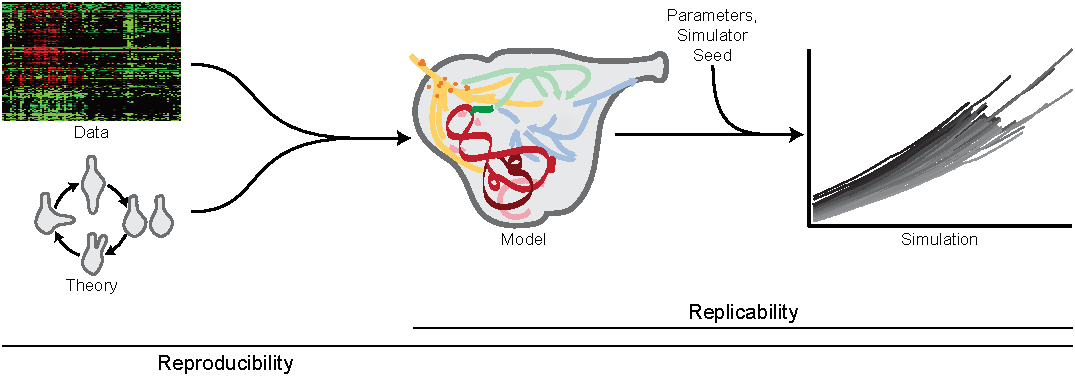
\includegraphics[width=\textwidth]{figure1/figure1}
% where an .eps filename suffix will be assumed under latex,
% and a .pdf suffix will be assumed for pdflatex; or what has been declared
% via \DeclareGraphicsExtensions.
\caption{Three requirements for reproducible systems biology modeling. (1) Every data source and assumption should be recorded so that each species, reaction, and rate law can be regenerated. (2) Every simulation parameter value should be recorded so that numerical simulation results can be regenerated. (3) Multiple simulation software tools should generate consistent numerical results. Reproducibility is a stricter standard than repeatability. Models are considered repeatable, but not reproducible, if they satisfy the second and third criteria.}
\label{fig_repro_diagram}
\end{figure*}

These standards and modeling software tools help researchers repeat most systems biology simulation experiments and reuse, modify, expand, and combine most systems biology models. However, these standards and software provide limited support for regenerating models themselves because they do not record all of the model design choices used to build models, including every experimental data source and assumption.

Furthermore, researchers have begun to develop more complex models which cannot be represented by the existing systems biology standards or simulated by the existing standards-compliant software. For example, several aspects of the recent whole-cell (WC) model of the gram-positive bacterium \textit{Mycoplasma genitalium} \cite{Karr2012} cannot currently be represented by SBML \cite{Waltemath2016}. In particular, SBML cannot represent the multi-algorithmic nature of the \textit{M. genitalium} WC model. In addition, no SBML-compatible simulation software program supports all of the SBML packages needed to represent WC models, including the Arrays \cite{watanabe2016efficient}, Distributions \cite{Moodie2015}, Flux Balance Constraints \cite{olivier2015fbc}, Hierarchical Model Composition \cite{smith2015sbml}, and Multistate and Multicomponent Species \cite{SBMLMulti} packages.

Here, we present a comprehensive vision for reproducible systems biology modeling, including WC modeling. First, we propose several requirements for reproducible modeling. Second, we outline several gaps in the existing standards and software for reproducible modeling and describe several new standards and software tools that are needed for reproducible modeling. Third, we describe several methods for verifying the repeatability of systems biology models.

\section{The Requirements for Reproducible Modeling}

There are three requirements for fully reproducible systems biology modeling (Fig.~\ref{fig_repro_diagram}). (1) Researchers should be able to regenerate models, including every species, reaction, and rate law, from the scientific literature. Consequently, researchers should record every data source and assumption used to build models. (2) Researchers should be able to regenerate statistically identical simulation results. Consequently, researchers should record every parameter value, algorithm, and simulation software option used to simulate models. (3) Researchers should ensure that multiple simulation software tools generate statistically identical simulation results. This is particularly helpful for identifying errors in simulation software programs. This requires standard model description formats that support all possible models, including WC models. This enables researchers to use different software programs to generate the same results.

\section{The Path to Reproducible Modeling}

Several new tools and practices are needed to help researchers reproducibly build and simulate systems biology models. (1) More comprehensive experimental databases should be developed to provide the data needed to build systems models.  For example, Karr et al. developed the WholeCellKB database \cite{karr2013wholecellkb} to organize the over 1,400 quantitative measurements used to build the \textit{M. genitalium} WC model. These databases should be machine-readable so that they can be automatically queried and used to build models. These databases should also use data models similar to that of predictive models to clarify the connection between models and their underlying experimental data. (2) New model design tools and Systems Biology Ontology (SBO) \cite{juty2013systems} terms are needed to record how models are built, including every design choice, assumption, and data source. Currently, researchers can use SBML annotations and SBO terms to record several common assumptions, such as the rapid equilibrium between free enzymes and enzyme-substrate complexes in Michaelis-Menten kinetics. However, many researchers do not utilize these annotations and the SBO does not represent all possible assumptions. Thus, researchers should develop model design tools which automatically record assumptions and data sources. The SBO should also be expanded to represent more assumptions. (3) The existing model description standards should be expanded to succinctly represent all possible models, including WC models. For example, to succinctly describe WC models, SBML should be expanded to support genomic sequences and sequence-based reaction patterns. (4) Where possible, researchers should use standard formats rather than to proprietary codes to describe models and simulation experiments. For example, researchers should use SED-ML to represent every software configuration option used to generate simulation results. (5) The existing standards-compliant simulation software programs should be expanded to support a wider variety of models. In particular, simulation software programs should be expanded to support the Arrays, Distributions, Flux Balance Constraints, Hierarchical Model Composition, and Multistate and Multicomponent Species SBML packages. Several simulation software programs, including BioUML \cite{Kolpakov2006} and iBioSim \cite{Stevens2013}, have already begun to support these packages. Unfortunately, most simulation software developers have insufficient funding to implement every package. (6) Researchers should systematically verify the statistical repeatability of every simulation software program and computational model. (7) New model verification tools should be developed to automatically identify errors in models. We developed a suite of simple tests to systematically error-check our \textit{M. genitalium} WC model. These tests checked for simple problems such as undefined species, reaction mass and charge imbalance, and inconsistent reaction rates among submodels. Nevertheless, we found this test suite invaluable for debugging our model. These tests should be generalized and new software tools should be developed to help researchers systematically evaluate such tests. (8) Every model, simulation experiment, simulation result, and simulation software program should be published open-source so that researchers have all of the information needed to reproduce reported results.

\subsection{Special Considerations for Stochastic Simulation}
Special care should be taken to ensure that stochastic simulations are repeatable because each simulation generates different results. We recommend that stochastic simulation software developers use random number generators (RNG) and seed these RNGs so that modelers can repeat results. This enables researchers to repeat not only statistical distributions, but exact trajectories, which is invaluable for identifying and debugging errors in complex models. 

Furthermore, we recommend that simulation software developers carefully review the documentation for RNG libraries and use methods which completely seed the internal state of RNGs. This recommendation comes from the observation that the \texttt{seed} method of the Python Mersenne-Twister implementation, unlike that of the C++ implementation, does not completely set the RNG's internal state. Thus, Python developers should use the RNG's \texttt{setstate} method to completely set its internal state, whereas C++ developers should use the \texttt{seed} method.

\subsection{Special Considerations for Multi-algorithm WC Models}
Multi-algorithm WC models strive to represent every gene and cell function by combining multiple submodels of individual cellular pathways, each represented using different mathematics and each trained using different experimental data \cite{Karr2015, macklin2014future, carrera2015build}. This multi-algorithm methodology is motivated by the desire to model biological systems as completely as possible, given our current knowledge, by simultaneously using fine-grained representations such as ODEs and coarse-grained representations such as Boolean networks to represent well- and poorly-characterized pathways. 

Multi-algorithm modeling is a new methodology which still lacks a strong theoretical foundation. Consequently, significant work is still needed to develop tools for building, simulating, and reproducing WC models. (1) The Hierarchical Model Composition SBML package should be extended to use the KiSAO ontology \cite{courtot2011controlled} to represent each submodel's simulation algorithm. (2) Researchers should determine how to concurrently integrate submodels that share state. Researchers are currently exploring several potential methods to concurrently integrate submodels, including shared memory and parallel discrete event simulation \cite{Goldberg2016}. (3) Researchers should develop a high-performance, reusable multi-algorithm simulator. (4) Additional tools should be developed to help researchers build and analyze WC models. (5) These programs should be integrated into a comprehensive WC modeling platform, but should be implemented as separate tools so that modelers can easily use alternative components and so that software developers can contribute to individual tools. We anticipate that this platform will enable more researchers to engage in WC modeling and accelerate the WC modeling field.

\subsection{Special Considerations for Parallel Simulation Software Programs}

Multi-threaded and multi-core programs execute individual instructions in a non-deterministic order that is determined by the program's operating environment. Multi-threaded and multi-core programs also non-deterministically allocate memory in ways that are determined by their operating environment. Special care should be taken to ensure that parallel simulation software tools are repeatable despite this non-deterministic thread execution and memory layout.

Deterministic synchronization is germane to WC models because hybrid models can exhibit the same repeatability problems as parallel computer programs. These problems occur when submodules attempt to exchange data or update shared variables. In the \textit{M. genitalium} WC model, the chromosome represents a single entity that can be accessed and modified by multiple submodules --- for example, to bind a protein to the chromosome. If two submodules attempt to bind a protein to the same locus on the chromosome, a race condition ensues. Such binding must be resolved deterministically if the simulation is to be repeatable. % Another example is utilization of a finite energy pool. At each timestep, the \textit{M. genitalium} model allocates available ATP molecules among its submodules according to each submodule's energy requirements. When the total energy requirements exceed the available reserve, a shortfall occurs and the energy resources must be partitioned among the submodules in such a way as to optimize the chances of cell survival. There are multiple strategies for performing this partitioning, but, if ranking is used to distribute energy, then care must be taken to ensure the ranking is repeatable.
We therefore briefly examine methods from computer science used to solve repeatability problems stemming from non-determinism caused by synchronization and memory layout.

\begin{figure*}[tb!]
  \centering
  \begin{subfigure}[t]{0.5\textwidth}
    \centering
    \begin{BVerbatim}
      -> x; 0.5 + vmax*(x^n/z^n) \
            / (15 + (x^n/z^n))
  x   ->  ; k*x/z

  z = 1*16
  x = 1.4925*16
  n = 4
  vmax = 10
  k = 2




    \end{BVerbatim}    
  \end{subfigure}%
  ~
  \begin{subfigure}[t]{0.5\textwidth}
    \centering
    % This file was created by matplotlib2tikz v0.5.4.
% The lastest updates can be retrieved from
% 
% https://github.com/nschloe/matplotlib2tikz
% 
% where you can also submit bug reports and leavecomments.
% 
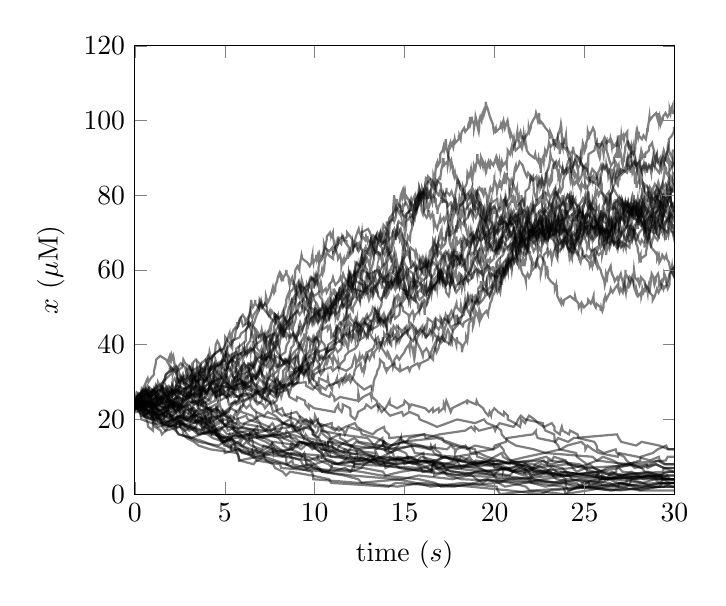
\begin{tikzpicture}

\begin{axis}[
xlabel={time $(s)$},
ylabel={$x$ $(\mu \mathrm{M})$},
xmin=0, xmax=30,
ymin=0, ymax=120,
axis on top
]
\addplot [thick, black, opacity=0.5]
table {%
0 24
0.101798882394875 23
0.331736770970644 24
0.474746114056171 23
0.505076550669378 24
1.39908125854676 25
1.72660316871354 26
1.7845951756382 27
1.81064466718327 28
2.06554246177701 27
2.14086005161984 28
2.15559728156685 27
2.36858724936124 28
2.58450694849738 27
2.88703645092384 28
3.08116429078927 29
3.08377782404649 28
3.11050415067516 29
3.32345293961214 30
3.34672655756192 31
3.48778255035819 30
3.58405778072195 29
3.59153790646317 28
3.61732612519941 27
3.76576465127414 28
3.98872951987883 27
4.12305219807304 28
4.78521256536269 29
4.95171959620937 28
4.98099948028958 29
5.48692412771024 28
5.55260529817165 29
5.61362622324645 30
5.87177564750557 31
5.9766646730256 32
6.32090529984002 33
6.33245439248521 34
6.33429430455878 33
6.61432441524495 34
6.62539632208014 35
6.67597408514023 36
6.70239905362509 35
6.74485432586885 36
6.7929152190681 37
7.12696951740697 36
7.26545942446307 37
7.31762860439307 36
7.34092570367561 35
7.46813399035171 36
7.57925527958561 37
7.59296890905227 38
7.59507665187674 39
7.60497658907559 38
7.69016677400432 39
7.73165982455237 40
7.81330922148174 39
7.90056756010829 38
8.04425703350393 37
8.16763023987305 36
8.44311163278388 35
8.50585003863986 36
8.59259873951465 37
8.63749840329366 38
8.67598130136889 39
8.83360137301432 40
8.83899485713667 41
8.84323055222794 42
8.88129996730241 41
8.95411083632597 42
9.03016138718001 41
9.15220634940494 40
9.25342651751355 39
9.36674277186123 38
9.51255059423698 39
9.51529887582497 40
9.51876106822616 39
9.56037383569344 40
9.58503148314306 41
9.66785875292662 42
9.84696807775493 41
9.90606767291492 42
9.95681879093578 41
10.1432131148807 42
10.1911629899092 41
10.1917680768397 42
10.2615071198733 43
10.3417194709526 42
10.3579647694655 43
10.3786745361695 44
10.4622608905625 45
10.4944293313375 46
10.537095922988 47
10.6198749193682 46
10.7724044965452 47
10.8516387835178 48
10.9041447983041 49
10.9316835382753 50
11.0207756799172 51
11.0492970155964 52
11.1511412817172 51
11.1780300505177 52
11.1938975715922 53
11.2094583985593 52
11.2407151399887 53
11.3141150212536 52
11.3368990381524 53
11.3463530962727 52
11.3760732818768 53
11.3771825650934 52
11.3786879525345 53
11.490661210981 54
11.7230734849138 53
11.8373182212927 54
11.8422317511094 53
11.8452044369754 54
11.9412673816472 55
12.0035128546584 56
12.0396456128791 57
12.117366531201 56
12.1641313699383 57
12.185741220763 58
12.2266216286044 57
12.2465490131671 58
12.2844835265088 57
12.6766148938416 56
12.7326942410423 55
12.7759489217888 56
12.8307908410295 55
12.8940993376853 54
12.9368164519083 55
12.9861936395065 54
13.134557133433 55
13.2136441604845 54
13.2172362236434 55
13.4386494598737 56
13.6328283958437 57
13.7081171180969 56
13.7407341731336 57
13.7412800629844 56
13.7417255572335 55
13.7421469415918 56
13.8752731237168 55
13.9002122537668 54
13.9401122667935 55
14.0471052364098 56
14.0506481618361 55
14.1372503465184 56
14.1373147912492 57
14.1695406112137 56
14.271895888177 57
14.3285635487297 56
14.4288500129402 57
14.4819370562204 58
14.5126212720268 57
14.5325057507862 58
14.5749966340988 59
14.6435136041626 58
14.6759345359481 59
14.7236832246073 58
14.7840528630128 57
14.8517917916747 56
14.9464542321398 55
14.9950034981784 56
15.0378094924077 55
15.0443005478498 56
15.0633381777531 55
15.0792778208145 54
15.1397591364361 53
15.2065002377599 54
15.2326191376621 55
15.2534265060933 54
15.3877431360542 55
15.5108188092184 56
15.558184180867 57
15.6676274899976 56
15.6699869691625 57
15.6805597334448 58
15.7191483738257 57
15.8099624549633 58
15.9282215887388 59
15.9294576204762 60
15.9495148852538 59
15.958330077444 60
16.0132307293579 61
16.0924772644864 62
16.1609285755104 61
16.169778248555 60
16.2130962388773 59
16.2370879915694 60
16.2495858196404 61
16.3283440868047 62
16.4720234065391 63
16.4895132614568 62
16.4917479933017 63
16.4944083637028 64
16.5341202879799 65
16.5594628884617 66
16.5764835532398 67
16.5820636902852 68
16.6800864538998 67
16.7290856985842 66
16.777002509242 65
16.7970634737573 66
16.8439706116125 67
16.8522858110933 66
16.8613893759672 67
17.0057426544866 66
17.0713968975899 67
17.0725156100255 66
17.2552425777691 67
17.2937422331645 68
17.296372208845 69
17.3076013621796 70
17.3724842163812 71
17.399706396781 72
17.4436551997254 71
17.4712171577868 70
17.477176090483 69
17.5087522539805 70
17.546285989509 69
17.6073322861901 70
17.6781121302486 71
17.710327304199 70
17.8428362760943 71
17.8666896675526 72
17.8785826869879 71
17.8810204339412 70
17.9011202687302 71
17.9388558432053 72
17.9766147596125 71
17.9783979623529 72
18.0595969691852 73
18.1056220421171 72
18.1061647545184 73
18.2908148864741 72
18.3093498244135 73
18.5002790480512 74
18.558788664162 75
18.6921705733846 76
18.8341756535285 75
18.9463230496679 74
19.0377546189369 75
19.0615536645021 76
19.1033944489808 77
19.1127272572421 78
19.1841730202932 77
19.2678298390636 76
19.285071637863 75
19.2928804359114 74
19.32281287391 73
19.3409815423947 72
19.3672254865072 71
19.3978216944159 72
19.4056772266945 73
19.4100147032512 72
19.4185293553413 71
19.4905739225308 72
19.4973976717011 73
19.540546064749 74
19.5567811565705 75
19.6020156834371 76
19.6860555682426 77
19.7035941318996 76
19.775869962057 77
19.7839795327579 78
19.7936588812768 77
19.8261024914755 76
19.8743563989632 75
19.9012433550509 76
20.0019060661312 77
20.0126302874892 76
20.0143945479849 75
20.0271048469 76
20.0996550518637 75
20.106932820443 76
20.1177426579352 75
20.2584712971286 74
20.3338472503496 73
20.3612348731771 74
20.4633709588179 73
20.4834882179045 72
20.4838978025003 73
20.5488519725078 74
20.56291655451 73
20.7219906428452 72
20.7795108131009 71
20.7825136855285 70
20.8064786856418 71
20.833207428632 72
20.8371008310452 73
20.9255387611226 72
21.1359355222013 73
21.2220317051997 72
21.2560072095104 73
21.2923849129934 74
21.3038394109611 73
21.311694208923 74
21.3913074942028 73
21.4342016493528 74
21.4786575259076 75
21.6271387111262 76
21.8611347227449 75
21.8731958096006 76
21.9386403788734 75
21.9555883119272 74
22.0000761350284 75
22.0993454389237 76
22.1829391259356 77
22.2413292739028 76
22.2523243434601 77
22.4725945220487 78
22.6233816641619 79
22.6516633713915 78
22.6704604686005 79
22.6863160657183 80
22.7225720654961 79
22.7722923699854 78
22.7810175139669 79
22.820237893842 80
22.8762636162986 79
22.9944355130794 78
23.1348340695549 77
23.255621274151 78
23.2747182531244 79
23.2938281669695 80
23.3636139646308 81
23.3854576284078 80
23.5173141144014 81
23.5239771022668 80
23.6330921798629 79
23.7214178577801 78
23.7594735433489 79
23.7720783700356 80
23.7798419775561 79
23.8572995391286 78
23.9858140081361 77
23.9977594028855 76
24.0283237824376 77
24.040439333918 78
24.0446085791399 77
24.081485340482 76
24.1209343351118 77
24.1467564936501 78
24.1723712934376 79
24.2063811782687 78
24.2654849177552 79
24.2959789932228 80
24.2998306253077 79
24.3013159420545 78
24.3476892018842 79
24.3588552484067 78
24.3815696473292 79
24.4546048203861 78
24.6032957306294 77
24.7826110494073 78
24.8875199945641 79
24.9627093470043 78
24.9720908541379 79
25.0343796164604 80
25.046574958223 79
25.0805560485118 78
25.1794833093345 77
25.1921282477195 78
25.196227675925 79
25.1991429627346 80
25.21643462471 81
25.2343483560718 80
25.2641645528776 79
25.3136743952594 78
25.3145593697843 77
25.4518016273185 78
25.4572023273609 79
25.5233930507394 78
25.5511260130601 79
25.5843061632197 80
25.6134118624434 81
25.6347448889223 80
25.7178988962062 81
25.7817304174267 80
25.875877776588 81
26.0472904366645 80
26.0503833518465 79
26.1030122090974 78
26.2136464619646 79
26.2619451695212 78
26.3098217084624 79
26.3300620881221 78
26.4005369384416 79
26.4210726140818 80
26.5354644709423 81
26.5620965733735 82
26.6710001971436 83
26.7000788277171 84
26.7315358735299 85
26.7896436888251 86
26.8269402876291 85
26.9823004715629 86
27.0066230730512 87
27.3663636549625 86
27.3990884386891 87
27.4316162158723 88
27.5629582245832 87
27.5653854226057 86
27.5889490658492 87
27.6076956879516 88
27.6438092094627 87
27.6603437445661 86
27.741447174957 87
27.7619395812641 86
27.7887753597086 85
27.7910176371155 84
27.8019433807246 83
27.8278576669123 84
27.8656730897047 85
27.8801545982527 84
27.8901513779244 83
27.8938036583653 82
27.9030911584203 83
28.0728171885681 84
28.0852062722756 83
28.1166797665404 84
28.1225313013003 85
28.1597696490325 86
28.1889502486672 85
28.1935721904018 84
28.2217617161839 83
28.3028523745309 82
28.3215548585641 83
28.5286178446479 82
28.5757280710042 81
28.5861382472413 80
28.6133536599045 79
28.7070342927958 80
28.7617732364398 79
28.764229352288 80
28.9366639985474 81
28.9489596222194 80
29.0332142304644 79
29.1099053079997 80
29.1309695397516 81
29.2259448658879 80
29.2735686024873 81
29.3177914476128 82
29.3381037190617 83
29.3705091965527 84
29.4055327264091 85
29.436397749987 86
29.4466166448855 87
29.4568824165095 88
29.5465229583438 87
29.5468327168975 86
29.6745787606502 85
29.6747790262008 86
29.7740611789574 87
29.9052551285421 88
29.9217027687747 89
29.9235567757353 88
29.9394672391104 89
29.958605276325 88
30 88
};
\addplot [thick, black, opacity=0.5]
table {%
0 24
0.285898347057625 23
0.619137773401076 22
1.08586666216687 23
1.09099783846379 24
1.20343166548929 23
1.34665839085637 24
1.53185728927038 25
1.64161937236052 26
1.92343532497991 25
2.21734374173819 24
2.25141885324031 23
2.53093946003561 24
2.93939012432396 23
3.10996652142852 22
3.13186203009255 23
3.28418167242111 22
3.33588694220684 21
3.33688540051148 22
4.09619402459477 23
4.49604631291563 24
4.5568374649502 23
4.57765691220235 24
4.69588120299265 25
5.10860166550955 26
5.46080839428655 27
5.76608989345163 26
5.99888891356961 27
6.01670099112214 28
6.02418851420553 29
6.26582420252174 30
6.28328000017894 31
6.31359570150732 32
6.35275203018201 33
6.36817703335027 34
6.50818618297189 35
6.56842895696164 34
6.67053728822871 33
6.71206616298148 32
6.84337997184341 33
6.91185837966483 34
7.02581544624794 33
7.08484357605575 32
7.27463931848178 31
7.33617544517978 32
7.41125360552826 31
7.63569133619243 32
7.69904510603667 31
7.87417073506953 30
7.92004250224702 31
7.98359769953576 30
8.15086021537708 29
8.23098451396378 30
8.36338449388445 31
8.3815331545924 32
8.46515848182225 31
8.71599576563151 32
8.72676589043994 33
8.74222635308903 32
8.87224692376524 33
9.00665826551074 34
9.2657359134886 33
9.37984856129697 34
9.6625222670656 35
9.66780266860506 34
9.69954889285024 33
9.75837377969266 32
9.86466416252817 31
10.0649328012934 30
10.1608756327346 29
10.3151193839408 28
10.3202100824467 29
10.6009932328376 28
10.7161442592402 29
11.2945774877523 30
11.3593936676586 29
11.4259886492406 30
11.6536895572395 31
11.6969723674924 30
11.9199824809007 31
11.9935262699989 30
12.1078630221517 31
12.2593278037107 30
12.4877514787819 29
12.7449184938491 28
13.1226791184812 29
13.2233887935902 28
13.2567509167313 29
13.2762779122815 30
13.330829383003 31
13.4363065501274 32
13.4764158079864 33
13.5917469838951 34
13.6222468096797 35
13.630466392968 36
13.8394612189398 35
13.8769752780166 34
13.9753894305743 33
14.0023963696729 34
14.0077989906924 33
14.1567761690033 34
14.4299688840887 35
14.4706013576013 34
14.7018978403003 33
14.7420519186806 34
14.7896996423894 33
15.1809563172237 34
15.2699675289625 33
15.3473386344155 34
15.7157104687532 35
15.8062149116953 34
15.8606502028992 35
16.2950467571326 36
16.4561165721815 37
16.4653421491147 38
16.5514815129558 39
16.6463248738122 40
16.6889547045063 39
16.7415380928261 40
16.7513912562006 41
16.8513584773766 42
16.9418060394565 41
17.0322209181217 42
17.2043644334841 41
17.2981845195683 42
17.3219278895751 43
17.4007776718292 44
17.4908550345234 43
17.4941340541581 42
17.4941731731729 41
17.5776884182572 42
17.6335668864689 41
17.6479201058144 42
17.8212619306333 41
17.8732979660296 40
17.8876165930219 41
17.9076920838523 42
17.9229602785596 41
18.1508575506045 40
18.1810929373273 39
18.1841193218305 38
18.2137081839522 39
18.285891838181 40
18.4099828501154 41
18.4134393994507 42
18.4811207666739 41
18.5067024303872 42
18.5365121967458 43
18.549134380922 44
18.5535311373442 45
18.6068650491842 46
18.7613437321098 47
18.8000477102202 46
18.8014640845312 45
18.8604079158925 46
18.8743323598183 47
18.9307067815436 48
18.9447908718886 49
19.0419324222053 48
19.1015520143794 47
19.122909776283 48
19.1531141164388 47
19.1710011758381 48
19.174002422354 49
19.2385804853352 48
19.2459656355938 47
19.352813494979 48
19.5379654485757 49
19.6323439817401 48
19.6489855510501 49
19.7135515382638 50
19.7488246649815 51
19.8399281891463 52
19.8921075935603 53
19.9991243041463 54
20.0599881005551 55
20.0689118982932 54
20.0785115467552 55
20.0822816129038 56
20.1366968598248 57
20.1377618054604 58
20.1807748816052 57
20.1885978720387 56
20.2425481823309 55
20.3121122105421 54
20.3394270234754 55
20.3603780801111 56
20.3783510748444 57
20.4083832925793 56
20.4175910190406 57
20.4433031476722 58
20.5204981590382 59
20.5294154139361 60
20.6283658090519 61
20.6639185213037 60
20.7188554549891 61
20.7462861912132 62
20.7803691792501 61
20.8243827659717 62
20.8352036448741 63
20.8866039486723 64
20.9132987366029 63
20.9522078611422 64
20.9907511605269 65
21.0181680969748 66
21.0184226555211 67
21.0942032253785 68
21.1105467320629 69
21.1144244799478 68
21.1433763011682 69
21.1501721002663 68
21.1700114755828 67
21.2268404089766 68
21.2374907719111 67
21.3157061923312 66
21.3201744214472 67
21.3247735197024 68
21.3497169602172 67
21.3860710131551 66
21.4520715395764 65
21.4960710782907 66
21.5142897479185 67
21.5816116665434 68
21.6660265925797 67
21.7285362189911 68
21.7585288991364 67
21.80042886299 68
21.8375073033061 67
21.8765784382158 66
21.8902475435677 65
21.942266635839 64
21.9569436647256 65
21.9651846746799 64
22.0696796976568 63
22.0969917844584 62
22.1348563904407 61
22.1354748153716 62
22.2768804832937 61
22.2963873373509 62
22.3700537630095 63
22.3703390248713 62
22.4291716790754 61
22.5680336148847 60
22.5690109240272 59
22.6119935988882 60
22.6541990332665 61
22.6909535224901 62
22.6942805955303 63
22.7343250801261 64
22.9295710278374 65
22.9332575504562 66
22.9492205875923 65
22.9665820503564 64
23.0920802002541 65
23.1068411436325 64
23.1261014854502 65
23.1305573418695 64
23.1681973550622 63
23.187295183632 64
23.1949917948479 63
23.242377768802 64
23.282474083474 65
23.3986328320351 66
23.4896303171652 67
23.517412747042 68
23.5826522379137 69
23.6735493544757 68
23.7105839399149 67
23.7133329932198 66
23.7932547017988 67
23.8096845935446 66
23.8246023793552 67
23.8390843000461 68
23.8433157409276 69
23.9037727360003 68
23.9246434362355 69
24.0188185732563 68
24.0373108318693 67
24.0761502772613 66
24.1208983228667 65
24.1449976081677 64
24.1860980184945 65
24.1997596828812 64
24.2317086068311 65
24.240744893753 64
24.3021332775997 63
24.3231980952607 64
24.3884320213229 65
24.4113290680629 66
24.4681594409119 65
24.6224477446732 64
24.6677237113489 65
24.6867820322043 66
24.7611435945029 67
24.7872643444031 66
24.9027100150703 65
24.927605773597 64
25.086061386527 63
25.2573067923341 62
25.2953139252608 61
25.3644349146226 62
25.42461023409 61
25.4493639686429 62
25.4523421593124 61
25.4902290596643 62
25.5093883062791 63
25.539434297302 64
25.5912270715778 63
25.6136012407288 62
25.6952863175395 61
25.7047198265478 62
25.7745071018968 61
25.8956898042719 60
25.944361182137 59
26.0204529149873 58
26.0969448555091 57
26.1233685297032 56
26.1715498338435 57
26.177276513964 58
26.1922947384092 59
26.2554891138642 58
26.2762320416927 59
26.3598424351917 60
26.451487327426 61
26.4732530904447 60
26.5239020656569 59
26.6193678070443 58
26.6749091549891 57
26.8131853794677 58
26.8799883757551 57
26.8869766098529 58
26.8904871248444 57
26.915508830299 58
27.0118324080307 59
27.0494107448407 58
27.1184018189274 57
27.1534956106642 56
27.1911681619894 57
27.2368418546698 56
27.2527760718412 57
27.2599343411459 58
27.2709485331658 59
27.2734044851957 60
27.2787935111956 59
27.4028524469469 58
27.5308158693012 57
27.530997233934 58
27.7210227643681 57
27.7300522073336 56
27.7761782465475 55
27.8519162927714 54
27.8710702097072 55
27.9168527617008 54
27.9789004111551 53
28.1418463596862 54
28.1540074723272 53
28.1988447330874 54
28.2160267972498 55
28.2765120039022 54
28.3574598193803 55
28.3762785795256 54
28.3865620630936 55
28.402258961488 56
28.54283519947 55
28.6137279148824 54
28.7935854416063 53
28.7938097245986 52
28.9031773572491 53
28.9651097490454 54
29.0283668921402 55
29.1156487090492 54
29.2168516654684 55
29.2367123178449 56
29.2369329133537 55
29.2624811279568 56
29.3627780457188 55
29.3766947936777 56
29.4042660767391 55
29.5759476357365 56
29.6239515927374 57
29.678899787932 58
29.7250682567153 59
29.8274929196095 60
29.8615423194389 61
29.8840155778022 60
29.8950457982988 61
29.9112276198238 60
30 60
};
\addplot [thick, black, opacity=0.5]
table {%
0 24
0.0382676390622353 23
0.114640910914623 24
0.198519832871391 25
1.30700731678533 24
2.03040052737984 25
2.32828878308523 24
2.5495578503978 23
3.05395196778594 24
3.28016873600988 25
3.50922811602374 24
3.54152250273488 25
3.79023419234057 24
3.81136388699977 25
4.05072977669515 24
4.45034383357865 25
4.49592831472498 26
4.59532679734434 25
4.6783376306386 26
4.82502712113116 27
4.9056155279679 28
4.93215867800917 27
5.19976053006705 28
5.36861075055158 29
5.4051038646462 30
5.553568185388 31
5.60980826560256 30
5.73391741389501 31
6.02124845181038 30
6.10101307849547 29
6.1416753038518 30
6.14275378154184 31
6.27174329692694 32
6.35904833393083 33
6.41886216309251 32
6.47331705052002 31
6.71592637892744 32
6.74981949640251 31
6.8855442545499 32
6.92112286450926 33
7.05329220231464 34
7.15938894995051 35
7.33143723012327 34
7.44462306964614 35
7.4689422037835 34
7.52198915614361 33
7.52484456512269 34
7.56003026506119 35
7.6253643623694 34
7.70846003929914 33
7.71326269303653 32
7.91458158077938 33
7.97941582888383 34
7.99063763019949 33
8.02272904001711 34
8.06351833955716 35
8.11468619778679 34
8.27581183515391 35
8.32067708033468 36
8.54827460398681 35
8.58535860795421 36
8.71521723219407 37
8.84378609345615 38
9.05482726039143 39
9.10635003586071 40
9.2032920407015 39
9.25394892009597 40
9.30909747548798 39
9.37577294982851 40
9.44609124645037 41
9.54944316153429 42
9.73077156954137 41
9.74728203578612 40
9.89338687247764 41
9.90030444519115 40
9.9638096737208 41
10.0252831452532 42
10.2132665608988 41
10.2410655792737 40
10.365335068826 41
10.5456808642885 40
10.5713459027081 39
10.6467914567667 38
10.690572220278 39
10.744625707195 40
11.0359512991159 41
11.0567616542274 42
11.1562633392881 41
11.1579081239333 42
11.1618635034193 43
11.185420754263 44
11.2085163185699 45
11.4188576940117 44
11.4563392459421 45
11.4798136955312 46
11.6997971621461 47
11.7489894469934 48
11.7498787180072 47
11.9570568367252 48
11.9937122336362 47
12.1734305519892 46
12.2616467211974 47
12.2857758088654 46
12.4118248556081 45
12.4618581541609 44
12.4652063696548 43
12.5040491930202 42
12.5415807077671 43
12.5519817997342 42
12.5569040846549 43
12.699192979307 44
12.7915869430757 43
12.9441639434899 42
12.9533608172596 43
12.9673388159999 44
12.9676736336505 45
12.9822139101046 44
13.1353321330847 45
13.1403390039677 44
13.4976000781409 45
13.5413123442173 46
13.558315511481 47
13.5663435404709 48
13.6458760466772 47
13.6757927894127 46
13.8199995781375 45
13.8550605667222 46
13.9703778081338 45
14.0284884731762 44
14.0306501376361 43
14.2280418363168 42
14.3469720584341 43
14.396789842552 42
14.5441512860596 43
14.5491879673362 42
14.586729557327 41
14.6461559300778 42
14.6627702141088 43
14.6891090965642 42
14.7112571162975 41
14.7976005271064 42
14.9270083664707 43
15.2387860858639 44
15.3996093962602 45
15.4912538724561 44
15.5260649695125 43
15.5300206674758 44
15.5370881420015 43
15.5396983311631 42
15.621229953728 43
15.6521572227077 44
15.7408916766205 43
15.8798389181064 44
16.1172579986759 43
16.1550354986527 42
16.4242336981873 43
16.4948859025777 44
16.498331814068 43
16.6088365424451 44
16.6942719292926 45
16.7083410038401 46
16.7462886052243 47
16.9908886840515 46
16.994125243595 47
17.0734689259741 46
17.1908000576213 47
17.4706265568107 46
17.5154221922623 45
17.6417962939869 44
17.6567017968004 45
18.0708466183162 46
18.2310091612013 45
18.2916897043427 46
18.6486093892999 47
18.6786053593425 48
18.7216943269136 49
18.8134595283769 50
18.8983559759812 51
19.0801400702052 52
19.0827117405177 51
19.199916732236 52
19.2144746723435 53
19.2693789639286 54
19.3955004481859 55
19.5706754249162 54
19.6709843031202 55
19.8577999229076 56
19.864006975114 55
19.874836080061 56
19.9193286684475 55
20.0448869960316 56
20.1098303463191 55
20.1570894328898 54
20.2629976651632 55
20.30277743003 56
20.3185891912218 57
20.3359753481043 56
20.3447463287226 57
20.3607984566447 58
20.3702183299519 59
20.4471877619576 60
20.4654605331684 59
20.4873438765355 60
20.5479391654709 59
20.5749945648748 60
20.6293917832797 61
20.6674803097896 62
20.73508011231 63
20.7478430629131 64
20.8720111898449 65
20.8880934864005 66
20.8899374593883 65
20.9922067526496 66
20.9996557246619 67
21.0179281856122 66
21.0755606285838 67
21.1663594257851 66
21.1726418457864 65
21.2314041399163 64
21.3196326222795 65
21.4419224094943 64
21.4626142795387 65
21.6489453588281 64
21.6898901356715 65
21.7262098832124 66
21.7580617125663 65
21.7604995909692 64
21.7748582478965 65
21.792760234719 66
21.7998700739118 65
21.8017933039233 66
21.8609564684986 67
21.8782906184529 68
21.9035166491022 69
21.9148247353709 70
21.9246150610269 71
21.9288345990891 70
21.9397452000708 69
22.0068509059879 70
22.0334340682548 71
22.1041446719173 70
22.1150199974045 71
22.1553889422766 72
22.2231613508445 73
22.3271934190483 72
22.4281793993527 73
22.5124972443913 74
22.548403035484 75
22.6290911884444 76
22.6425260212363 77
22.7110511418816 76
22.7788889435033 75
22.8014834414696 76
22.8017259900048 75
22.8329774806946 74
22.8489936527281 73
22.90107122029 74
23.034768572368 73
23.1194841057477 74
23.1207897248588 73
23.1562984248906 74
23.1570431114079 75
23.2130178877119 76
23.2202623673334 77
23.2840329876708 76
23.3203781658713 75
23.3503586724321 74
23.3610669434058 75
23.3691996449997 76
23.4050501176378 77
23.4071439791469 76
23.5005193480885 77
23.6680645824303 76
23.7137402007491 75
23.7684478579115 74
23.8347470502497 73
23.86365219562 72
23.8846189673406 73
23.8898342056095 74
23.8973614691243 75
23.9123181997377 76
23.9149609808353 77
23.9531349287506 78
23.9812438881623 79
24.0763141900847 80
24.1916989263663 79
24.1925060159392 78
24.1952909992526 77
24.1990082309614 76
24.1996742683688 77
24.2103237301317 78
24.3189321217814 79
24.3494825101879 78
24.3686358306595 77
24.4052959008076 76
24.6784071047661 77
24.6861648173868 76
24.7598692897081 75
24.7850207606242 74
24.8046951567067 75
24.8658924901135 74
24.8924194947978 75
24.9404079341004 74
24.9706726881554 73
25.0883757136965 74
25.2694575547024 75
25.3255641879396 74
25.3558326599176 75
25.3900556595164 74
25.4171969876872 75
25.4395689048024 74
25.475412043592 73
25.529388184451 74
25.5781199012845 73
25.5894494734558 72
25.6238193605645 73
25.6454916682204 72
25.7723448548622 73
25.8112352260463 72
25.8166804561232 71
25.8591855199418 70
25.9618163855578 71
26.1066810965216 70
26.1930990590043 71
26.1975726986233 72
26.2165897370187 71
26.4001940975624 70
26.5428723475114 71
26.5865501862675 70
26.6128512930639 71
26.6334442720083 72
26.6427281665043 71
26.7181560662547 72
26.7907616244875 73
26.9437240947095 72
26.9523844939252 73
27.0260586031111 74
27.1591104979284 73
27.1636280435844 74
27.2021226767557 75
27.3285865824275 76
27.3799113446588 77
27.4073077366105 76
27.4959490773384 75
27.5845338982856 76
27.6386585854347 75
27.6966631604785 76
27.7393674787636 75
27.7988080068412 76
27.8368178140253 75
27.8680816380164 76
27.8699105762663 77
27.9042896171434 76
28.0599636373806 75
28.1148195980621 76
28.2743202452318 75
28.2782022097224 74
28.3216834556577 73
28.345560829394 74
28.4663337109982 75
28.5266436379698 76
28.6237445017367 77
28.6747549616019 78
28.7254442070898 77
28.7908267855865 76
28.8367709501581 77
28.8934834194084 78
28.9082388494808 79
28.9346934012207 80
28.9353487611155 81
29.0168110655602 82
29.0710670094892 83
29.0905693226536 82
29.1238644658547 83
29.1789028230189 82
29.2045247098315 81
29.3565393468197 80
29.3671509440927 79
29.3842853670626 78
29.4296435790225 79
29.4481958248885 80
29.4498723494455 79
29.490722912382 80
29.5647681869131 81
29.5835275621121 80
29.662421296858 81
29.6699791499737 80
29.671516980794 81
29.7786565625688 82
29.9040314113494 81
30 81
};
\addplot [thick, black, opacity=0.5]
table {%
0 24
0.106531364858955 25
0.133943945465091 24
0.143800046596781 23
1.19844080681553 22
1.20540314235741 21
1.58472318746164 20
1.76351754659647 19
2.01346733944947 20
2.1028569183488 21
2.33998769228994 22
2.56590135509346 23
2.82932999770627 24
3.02412558034501 25
3.30626238769531 24
3.64949203274272 25
3.93736579866891 26
4.1255827074099 27
4.14057559914632 28
4.46342608089976 27
4.46701143351461 28
4.4954219996181 29
4.56117811969985 28
4.56302894098877 29
4.70912612213661 28
4.73990408402303 27
4.7547387991635 28
4.84468179971069 29
4.86208016265574 30
4.98543930662563 31
5.02735646082044 32
5.17724496557317 31
5.21895929045546 30
5.24846915025418 31
5.33674115182028 32
5.5586190777168 31
5.84727815310289 32
5.88429279682156 31
5.95652641824471 30
6.2045343187308 29
6.37614837508963 30
6.46362519681646 31
6.56180952895282 30
6.73948519771027 29
6.85709475916931 30
6.90356019073691 31
7.08849198139168 30
7.16241995410084 29
7.19946596109529 30
7.2295433558206 29
7.4817348571142 28
7.86538377276216 27
7.88151296345216 26
8.10492133573297 27
8.14163393693689 26
8.20444826285747 27
8.25050988847676 28
8.27686906877941 29
8.34909646593919 30
8.64001394240005 31
8.74870329800832 32
9.03177021221409 33
9.18081165526538 34
9.3128344098633 33
9.31880610726003 34
9.52275824721466 33
9.54322597212309 32
9.65521465940195 33
9.67749797825628 32
9.68297003682844 31
9.69513379584621 30
9.83267816210336 31
9.86244861174246 32
9.91768653672984 31
9.97697037100589 32
10.2746023593328 33
10.3402337435219 32
10.5011013968266 33
10.5048483695129 34
10.5850763642574 35
10.6304473802457 36
10.680780890529 35
10.7502132545693 36
10.7900904983165 37
10.9940450849842 38
11.1544660998216 39
11.2744974256032 38
11.4804721547779 39
11.4949840372614 40
11.508271076617 41
11.5093382109667 42
11.5546683836715 43
11.5592729065725 44
11.7416753632493 45
11.7976814396855 46
11.8542589594321 47
11.8839998563344 46
11.9277407011848 45
11.9408250355502 46
12.1006032948872 45
12.2688077064591 46
12.541993113318 45
12.5582363635664 46
12.6892336261598 47
12.8608717978139 46
12.8856598395103 47
13.0971869841003 48
13.1861389469127 49
13.2313501839633 50
13.445394198726 49
13.4811859028247 48
13.5253322898458 47
13.5833709331048 48
13.5893073501149 47
13.6474916490298 46
13.6621696640289 47
13.854044358555 46
14.0222497211768 47
14.0927703801067 48
14.2210088656833 49
14.24529364496 48
14.2614989712933 47
14.3210822247419 48
14.3967805648356 49
14.4025654361528 50
14.4141093701021 51
14.4472073455616 50
14.4662447024145 51
14.4958330179936 50
14.7709773154084 51
14.8873713058735 50
14.9217204253284 49
15.2133465109707 48
15.2358478668849 47
15.3036775861475 48
15.4422960101156 49
15.4995026000109 48
15.5180077306653 47
15.5901446648922 48
15.8109149272051 49
15.9049828348576 50
15.9745384333219 51
16.0756927637545 52
16.2024692198528 51
16.2358048683371 52
16.3694551472852 53
16.3804402600968 54
16.4216951870385 55
16.4385499903577 56
16.4962132346555 55
16.6717835250046 56
16.8122065264791 57
16.8623162410213 58
16.8759433064336 59
17.0140303445416 60
17.1197246526149 59
17.1222809656113 58
17.1326526780376 57
17.1430692728486 56
17.2802125277924 55
17.3032390603746 54
17.4467339797614 53
17.4974337928212 54
17.4996914377524 55
17.533390275482 56
17.5807808762475 57
17.631097871006 58
17.6843636410162 57
17.687653192543 56
17.7936920572754 55
17.8676174768131 54
18.0261673796424 55
18.0537437993655 56
18.1410105978367 57
18.1630703894738 56
18.1844545970523 55
18.2298238320934 56
18.2522656855111 57
18.3995260096048 58
18.5188699796798 59
18.6727653892703 60
18.6791447077465 61
18.6951052748737 62
18.7355895339645 61
18.8180131201124 62
18.9053936058057 63
19.0613423989961 64
19.0904956203407 65
19.2377389155356 66
19.2421661056491 67
19.3202792932327 66
19.3698357022133 65
19.4831695330741 66
19.512665197245 67
19.5275582434678 68
19.5350775817571 67
19.5803349633386 68
19.5966911640932 69
19.6516089663541 68
19.7184775228336 67
19.7583254117656 66
19.7972302684207 67
19.9486570801518 68
20.0358595493112 69
20.0578068748338 68
20.0827312866049 67
20.0875719689855 66
20.1162294832303 65
20.2390930795766 66
20.2853210347319 67
20.3279977669869 68
20.3569452695081 67
20.3759520701385 68
20.4228010177593 69
20.4371056188572 68
20.569744343529 67
20.7426099791389 66
20.7608073559213 65
20.7767883603314 66
20.8650797382758 67
20.8788768099162 66
21.0122331467524 67
21.0159187222881 68
21.1058447853469 69
21.1904694225443 68
21.2288531711145 67
21.3128501681225 66
21.3265275957475 67
21.352712635359 68
21.36260255267 69
21.3812377929028 68
21.3952604853936 69
21.4313004167567 70
21.5172799614601 69
21.518236371037 70
21.6024881975217 71
21.6793334810687 72
21.7044381691411 71
21.7477136580129 72
21.8552800889887 73
21.9627592667238 72
22.0330934001387 71
22.0380472240179 72
22.0438002267138 71
22.0547230854441 70
22.0790863816647 71
22.1060704693343 70
22.13323283207 69
22.1721603174419 70
22.3015359166605 71
22.3090983464173 70
22.3298222381915 71
22.3606812888947 72
22.4516076133282 73
22.5461725388601 74
22.6118699756835 73
22.6339783887066 74
22.6833792544454 75
22.7230707696415 76
22.831900786984 77
22.8418685224391 76
23.0259757382779 77
23.0413023860599 78
23.0489465765187 77
23.0638143271726 78
23.1758632265529 77
23.220673201939 78
23.2750870095776 79
23.3895839827679 80
23.393533647397 81
23.4026576142653 80
23.4318249899361 79
23.4328551659848 80
23.4424564289747 79
23.4791474847695 80
23.5854831421494 81
23.6282602760857 82
23.6791197434369 81
23.7797925055646 82
23.7914779676859 83
23.8035949498967 84
23.8818471792603 85
23.973045333897 86
24.0401291893728 87
24.2272772331031 88
24.2384011344334 87
24.2631337370198 86
24.2754152838803 87
24.3857079775032 88
24.4541079039951 89
24.4772040220897 88
24.4835608088413 89
24.5525972345648 88
24.6112871256356 87
24.7216139156908 88
24.7935630982262 89
24.8441181025487 88
25.1416354058937 87
25.1978636576134 86
25.226142535621 85
25.3169287237465 84
25.3237650091625 85
25.3588046982382 86
25.4277535828624 87
25.6126382145667 86
25.6708470262959 85
25.7727495114179 84
25.777659682719 83
25.8538644042321 84
25.8804398790292 85
25.8984261879935 86
25.912545101256 85
25.9492888194036 86
25.9633584800664 87
26.0162415513166 88
26.0959778369061 87
26.2367723789919 88
26.3012683837006 87
26.3047378988296 86
26.3223589329442 85
26.3769170971755 86
26.4106044263278 85
26.4604215076475 84
26.4680099733319 83
26.5344509910879 84
26.595001626761 85
26.6741280296669 86
26.7025097820352 85
26.7335628798954 84
26.8250982226446 83
26.8431561822006 84
26.8476643079299 85
26.882585354444 84
26.9091661868298 85
26.9369526540422 84
26.9435062181197 85
27.1483721850934 86
27.3427668113429 87
27.3494327457146 88
27.3739808929972 89
27.3995913364022 90
27.5640093704145 91
27.5666425612701 90
27.5928185029193 89
27.5984263007402 90
27.6115170962291 89
27.6324514410799 88
27.6331428692307 89
27.7102727719006 88
27.8068434864808 89
27.8249117429705 88
27.8465337198114 89
27.8735795943511 88
27.8880601115083 87
27.9131664820306 88
27.9616936463275 87
27.962754025161 86
28.010488389589 85
28.014564453814 86
28.0433343109135 87
28.0926196798468 88
28.0991074778168 87
28.1953902279202 86
28.2303690872556 87
28.2759613346212 88
28.2815864055549 87
28.4132377567667 88
28.460190880778 87
28.4680140482529 86
28.5012828809016 87
28.6312565948926 88
28.7426423403551 87
28.7599826591504 88
28.7885132473337 89
28.8133202013291 90
28.8507961612844 89
28.8600655557943 90
28.9122826370751 89
28.9418236098129 90
29.0224664002518 91
29.0379280814618 90
29.0652909472919 89
29.1827566510932 88
29.2809108615631 89
29.3256127376793 90
29.4111717817958 89
29.4229614017961 90
29.5913430154514 89
29.6513340038978 90
29.6979084058315 89
29.7109163516765 88
29.7485190203855 89
29.8389581495026 88
29.8891404884716 89
29.8986802443955 88
29.9402308890534 89
29.973866663838 88
29.9792401437756 89
30 89
};
\addplot [thick, black, opacity=0.5]
table {%
0 24
0.535532638080703 23
0.608344547226046 24
0.796369877557326 25
1.18455152225823 24
1.28580152306378 25
1.52020702009015 26
1.66655202291341 25
1.85459353966259 24
1.88500827875259 23
2.3418076478258 24
2.43216250873392 25
2.52162573396002 24
2.75179363095473 23
3.08636738197609 22
3.18942347471594 23
3.27923409087089 24
3.33179243370548 25
3.51577820889851 24
3.56134805552065 25
3.57167778617464 26
3.70574980829669 27
3.72844567454457 28
3.78371274227963 29
3.85319365449819 28
3.882551315492 27
4.04572750886015 28
4.21066625002503 29
4.28185049869862 30
4.59677852721672 29
4.68146275611641 30
4.79321636908033 31
4.82348251978362 32
4.94895797170855 33
5.25523708761926 34
5.35281029799663 33
5.42741432599684 32
5.4867919971321 31
5.4979776567082 30
5.60552339303753 31
5.63042451608114 32
5.64796027109321 31
5.68010226955691 32
5.79457024162651 33
5.92747664967105 34
5.95666736409672 33
5.98838351912509 34
6.07793109751924 35
6.13342225904545 34
6.20596472938129 33
6.30217004181844 34
6.36755541457539 33
6.42369446735537 32
6.4636038739051 31
6.55346980405166 32
6.71955648533977 31
6.78802132974773 32
6.91145147448987 33
6.98828310235546 34
7.02503165369429 33
7.07982708710291 32
7.12436373841606 31
7.13386819224879 30
7.31500088942857 29
7.3663159537506 30
7.38884576377134 31
7.79326652279267 30
7.93282599070089 29
7.94348420735703 28
8.05867529456022 29
8.07651027476303 28
8.48610703509995 29
8.789713889516 30
8.96348055784188 31
9.12988838129732 32
9.20740901484182 33
9.26508119405869 34
9.50626317763349 35
9.51343735632026 36
9.61789562539682 35
9.63645828860594 34
9.8090521367414 33
9.927494158166 32
9.93298211784946 33
10.1521951350535 34
10.2481587943278 33
10.2812668771556 34
10.3391689410258 33
10.8951943083028 34
11.0099408076069 33
11.2549618630652 34
11.7596689370204 33
12.0464025748099 34
12.1181516139019 35
12.1604890938669 36
12.2286424793741 37
12.3057588830582 36
12.3065242783696 35
12.4462029839521 36
12.4931877326813 37
12.5185193767958 36
12.6530241288046 37
12.7517244657106 36
12.8192902516207 37
12.8397504062428 36
12.9240813565469 37
12.9319120149403 38
13.2545458799635 39
13.334141386603 40
13.3694620454671 41
13.3905586823979 40
13.4056965872764 41
13.6523873694474 40
13.671507931331 41
13.6842499568731 40
13.7782668051322 41
13.7816947100379 42
13.7900407840078 41
13.8795632454411 40
13.9534997268455 41
14.0956470591404 42
14.1583365832938 41
14.1753766194401 42
14.1781654538813 43
14.2410340481368 44
14.3147451850184 43
14.3400789595458 44
14.3804840347611 45
14.5233188568462 44
14.5753189335167 45
14.7805913847582 44
14.842004793756 43
14.9165123100855 44
15.1048068355083 45
15.1326261229223 44
15.1475563293066 43
15.2656966367238 42
15.4561312556814 41
15.579900984735 42
15.6549182767018 41
15.7071553775001 42
15.85447133872 43
16.0734152316396 44
16.174248101856 45
16.2055166261677 44
16.2422731082649 45
16.2597964358548 46
16.2846965589588 47
16.557663547047 46
16.5726599292595 45
16.6302615396738 46
16.6721392565035 45
16.7030943030255 46
16.7417104151489 45
16.8890822287459 44
16.9943112596434 45
17.0382809384223 46
17.0701779249768 45
17.1926489556609 46
17.2354080368694 47
17.2757208351304 48
17.356209269373 47
17.3691812128708 48
17.3721688923505 47
17.4629618944244 46
17.5932256343355 47
17.7037640196948 48
17.7645376294803 47
17.8004820430987 46
17.8486611477026 47
17.8769948279366 48
17.8839331945206 47
17.9677951853393 46
17.9977059938126 47
18.2877867492013 48
18.3200133912015 49
18.3257940381262 50
18.3292805529901 51
18.3590152337847 52
18.3913331105377 51
18.4250176263735 50
18.5335133209147 51
18.5385538425583 52
18.5899127485868 51
18.7099488665826 52
18.9700400971829 51
19.0084344784545 52
19.0184128507707 53
19.0821128641156 54
19.0823740123638 55
19.2245239026147 56
19.2296307661258 57
19.2345219463853 56
19.2419624393209 55
19.2587484723781 56
19.3829257125929 55
19.4483912644797 54
19.5132163134033 55
19.5426118352002 56
19.5641886903545 55
19.5718347769426 54
19.6942619126413 53
19.808437161432 54
19.8266018797133 55
19.8758009608994 56
19.9777221175894 57
20.0046192004454 58
20.0533247428668 59
20.154495825549 60
20.1666333948483 61
20.2531824081896 60
20.2583839734399 61
20.3059994742946 62
20.3292293753797 61
20.434319431385 60
20.4859926558403 59
20.5070882524862 60
20.6493327387296 59
20.6828166551364 60
20.6890099432987 61
20.7911634995115 62
20.8012376339054 63
20.8782253610317 62
20.9329664606468 61
20.9554291322483 60
20.9802277802978 61
21.0709736975476 62
21.0936163211214 63
21.2192544576643 62
21.2307033851729 63
21.2508672827282 64
21.3113335229745 65
21.352290103551 66
21.3533101738363 67
21.4930199213848 68
21.596825727297 67
21.651903090469 68
21.6630082119803 67
21.7187632826832 66
21.8825886359256 65
21.8885538988306 66
21.9845857220376 67
22.1048138631037 66
22.171237881289 65
22.2897355979405 66
22.324923408894 67
22.3610252408367 66
22.3802993662277 67
22.3957616978257 66
22.4174384264312 65
22.482005192321 66
22.5766605482525 65
22.6036346703524 66
22.6864892367633 67
22.7630567035413 68
22.7789013904107 69
22.8745872792387 68
22.9791135026248 69
23.0560562874575 70
23.1286158106565 69
23.4594948680737 70
23.4613497028552 71
23.4619216291909 70
23.4792022706979 69
23.5117875731552 70
23.5959961204213 71
23.6063011820756 70
23.6242333255782 69
23.6289352912866 70
23.6404210433684 71
23.719137082787 70
23.7277336510255 71
23.7613552390741 70
23.9052179100281 71
24.0074183096681 70
24.0074884677795 69
24.0186039496134 70
24.1454379025509 71
24.1958942949946 70
24.1970894162771 71
24.2262889989211 70
24.3145414508347 69
24.5605009484641 70
24.5905465842368 71
24.5920355648821 72
24.6265736856114 73
24.6686151443586 72
24.7317513187612 71
24.7414793882727 72
24.8070219762914 73
24.8125813388256 72
24.8291130441995 73
24.9109530358163 72
24.974603309007 73
24.9863454439009 72
25.0703739060421 71
25.2620774265801 72
25.2939644432701 71
25.3228485581276 72
25.4212654635654 73
25.4886738241679 74
25.6589023641184 73
25.8128758835863 74
25.9602209558626 75
26.0107100040374 74
26.0810829878877 75
26.1732743188459 74
26.2288233594165 75
26.2358479816036 76
26.3357115234605 75
26.3678544676717 76
26.3870548851769 77
26.4109453405937 76
26.6118290155233 77
26.6178505149597 78
26.6255260580568 77
26.7044978998059 78
26.7238646759538 79
26.7338107010899 78
26.739228986926 77
26.7542986747535 76
26.7826307191434 77
26.8396007908767 78
27.0113056759056 77
27.0691463516296 78
27.0697336524226 79
27.0813302657522 78
27.199067457784 77
27.2090521546595 76
27.3013240976472 77
27.3271214416225 76
27.386321759183 77
27.4180312459945 78
27.4561557414047 77
27.4615305656033 76
27.5388682389899 75
27.6136931599977 76
27.6287399784355 77
27.6494276202346 76
27.6790149827044 77
27.7478486399835 76
27.891312696067 75
27.9795686630017 74
28.0021010532331 73
28.0087045195179 72
28.0387207365369 73
28.0391373881214 74
28.0591007584893 73
28.0729677909676 74
28.1416882049841 75
28.1543530978868 74
28.2383416317649 75
28.2547019065624 76
28.2825794028263 77
28.2829863602068 78
28.2946927503137 79
28.3226853454812 80
28.3454190083452 79
28.3819984065062 80
28.478754801361 79
28.5339786501528 80
28.5465194373632 81
28.5689351935163 80
28.6800533775572 79
28.6810117520053 78
28.7314652439996 79
28.7439028624383 78
28.811407731813 79
28.9988453084772 78
29.0200604129201 79
29.0216140985712 80
29.0392915030552 79
29.2102418444735 78
29.4961927919776 77
29.6020548811303 78
29.6178080776138 77
29.6327306268872 78
29.7164834377384 79
29.7168238574033 78
29.7191688136612 79
29.7449014545544 80
29.7496497096945 79
29.7664972062226 80
29.7786590360675 79
29.8305321303616 78
29.9019332557551 77
29.9116546156681 76
29.9755927387397 77
30 77
};
\addplot [thick, black, opacity=0.5]
table {%
0 24
0.219077299470484 23
0.874726731157018 24
0.984507385093016 23
1.14073369718679 24
1.18855597425894 23
1.47704616349363 22
1.592334652518 21
1.69838678183645 22
1.83865608668158 21
2.14521876794283 20
2.72811290389541 21
2.7446699107466 20
3.29281130136392 19
3.49114403722657 20
3.70387373760782 19
3.72335464217382 20
3.85453177022081 19
4.16879743842016 20
4.30830272086292 21
4.50173093332079 20
4.63915276361081 21
4.66474495142244 22
4.74362314807613 21
5.22838434971892 22
5.29487098494017 23
5.47199007004946 24
5.77729243169963 25
5.83299402392891 26
6.6933301494809 27
6.93748287111139 28
7.01688455186672 27
7.11210535909701 28
7.6297754273333 29
7.71394014202684 28
7.86231217937696 29
7.88978033145512 28
7.91596092798599 29
8.07772370115008 30
8.14819431560749 29
9.49476591508072 30
9.51901389666918 29
9.89273981991459 28
10.067128700521 29
10.1921854912743 30
10.1976941146135 29
10.2216231554587 30
10.247070707763 31
10.7040986894822 30
10.733970419993 31
10.7631565881366 30
10.851457068328 29
10.9641044030809 28
10.9793730804558 29
11.1644763778232 30
11.2372199041371 31
11.2519938435753 30
11.4886323778696 31
11.5550880637191 30
11.5878289648621 31
11.7320141273136 32
11.7741561149203 31
11.9439700927174 32
12.0754051096003 31
12.1908941799044 32
12.2098003299071 33
12.3103948702712 34
12.5531998170981 35
12.5674917141415 34
12.6300933408008 33
12.7350377995735 34
12.7491578205239 33
12.8044922607322 34
12.8076186406674 35
12.8593771605027 36
12.944441004355 37
13.0456959389524 36
13.1311083499281 37
13.196752483756 38
13.2877309319773 37
13.3107355375467 38
13.462985531859 39
13.4688535690564 40
13.5855620400195 39
13.614236151771 40
13.6143556636053 39
13.7178653843469 40
13.7402389105822 39
13.8747169394984 38
13.9969350136397 37
14.0401122270893 38
14.1429515663265 37
14.1472724719895 36
14.1502839427204 37
14.2360192577694 36
14.3163470868717 35
14.3469166610299 34
14.4018534376874 35
14.4285341646771 36
14.568512611149 37
14.6954385200841 36
14.8298337446173 37
14.9849133937818 38
15.0694855788415 39
15.2299614378147 40
15.2719645902939 39
15.2761373791343 40
15.3235009200291 41
15.3452729055428 40
15.4275625177091 39
15.4726610648714 38
15.5053323989234 37
15.5226233166526 38
15.5603301418293 37
15.5889306074864 38
15.6064177767971 39
15.6249931118846 40
15.6341429369094 41
15.7458839305797 40
15.857924072888 39
15.9422792625458 38
16.0079560143839 37
16.0371817454206 38
16.2082602593006 39
16.3276043262398 38
16.3723254717628 37
16.5740577047181 36
16.5825136098607 37
16.6220914258482 38
16.7201904151989 39
16.7723668070033 38
16.8755263899449 39
16.9157360197199 40
17.1183704885057 41
17.1310860436573 42
17.2402709168685 41
17.5433290315836 40
17.5783797446941 41
17.6096809137615 42
17.6487531031813 43
17.7081809253194 44
17.8949107917158 45
17.9594063457652 46
17.9704670781781 47
18.0642254526917 46
18.1449007552066 47
18.1972430603967 48
18.2814612801133 49
18.3597940075018 50
18.4258089993074 51
18.4703966677118 52
18.5145380840288 53
18.5469120434836 52
18.642186285742 53
18.7326024445382 52
18.7664417373244 53
18.8804668198183 52
18.9285436334794 53
19.0639625565929 52
19.1194287049547 53
19.1231376548413 54
19.3506524565807 55
19.3547062376036 56
19.3671795465195 57
19.4868407337162 56
19.5407571354936 57
19.5615395038379 56
19.5953640241628 57
19.6033374617693 58
19.6805012251613 59
19.8168232966023 58
19.842052905693 59
20.1493405079593 58
20.2610041192021 59
20.3111884220672 60
20.3579284490826 61
20.5023283918512 62
20.670761490496 63
20.712595469238 62
20.7487258654773 61
20.7892882863739 62
20.8685839182894 61
20.9144703251545 62
20.9769092796835 63
21.0798248044444 62
21.1400326386595 63
21.2229418410886 64
21.3082140261714 63
21.3523680882204 64
21.3966691071686 63
21.5390191295153 62
21.550630778878 61
21.557638424991 62
21.5835475495647 63
21.6558755019293 62
21.6569220627239 61
21.6953012812425 62
21.736458845841 63
21.7406285145998 64
21.8012828278496 65
21.8056199176452 66
21.8343871452507 67
21.8498603526563 68
21.8944171729013 69
21.9515342284058 68
22.0252558201438 69
22.2592357901018 70
22.2623491584481 69
22.3642983694783 70
22.3821446143645 69
22.4023074666576 68
22.4256394320177 69
22.4921980774694 70
22.5200850844812 71
22.5550426108929 72
22.5967093585811 71
22.6072767520039 72
22.7102629102039 73
22.7185771735357 72
22.7602221028549 71
22.9343059087575 72
22.9379422994038 71
23.00047084761 70
23.0027024683544 71
23.0052557935118 72
23.0195197296865 73
23.0229868652172 72
23.0237030323123 71
23.1273722948029 72
23.1336349040229 71
23.2460487513549 72
23.3132967545309 71
23.5748102888905 70
23.6702711144515 71
23.7121595763511 72
23.7207098662967 71
23.7436162863734 70
23.9133810665058 71
23.9328420378107 70
23.9485176802361 71
24.0045675520784 70
24.0654798436968 69
24.1348443269897 68
24.1864830964586 67
24.2446384423911 68
24.2963895827549 67
24.3314100788339 66
24.3469339514487 67
24.4311889172782 66
24.5823312413246 65
24.6711949449604 64
24.686454503344 63
24.7773890352169 62
24.8052415135752 63
24.8541996335799 64
24.8603840705517 63
25.0899181415745 64
25.3063040246593 63
25.3115934816319 64
25.3243551818047 63
25.3479198348013 64
25.4121147099172 65
25.4230184581529 64
25.5194800581721 65
25.5400128448416 64
25.58808150183 63
25.6252639870509 64
25.62933586721 65
25.7879417902753 64
25.9808021776905 65
25.9826512186854 64
26.0335150419771 65
26.0729029782142 66
26.0768975064018 67
26.0991926081744 66
26.1938027316272 67
26.1967072749805 68
26.207629147165 69
26.2200285330998 68
26.4261070024209 67
26.4877110924778 68
26.7895174594585 67
26.894544902694 68
26.9018582555506 67
26.9417594289993 68
27.1612911475116 67
27.1741123098335 66
27.2331717224534 67
27.4958865569285 66
27.5119294647909 67
27.5214399341313 68
27.5340134563167 67
27.6610117990774 68
27.7325610483062 69
27.7757664401168 70
27.7885826555839 71
27.8172538773013 70
27.9656364502739 69
27.9856057632762 68
28.107773263127 67
28.1774489666112 68
28.3323864528943 67
28.3341619731266 66
28.3599404925487 67
28.4000416355969 68
28.5035803770367 69
28.6200218265164 70
28.6468092886807 71
28.739859955513 72
28.8237765135384 71
28.9278179001419 72
28.9310371050295 73
28.9493274849851 72
28.9821887914385 71
29.0131968682963 72
29.0388200883518 73
29.0532093504236 72
29.0974095291786 73
29.1825347851813 72
29.2489667147804 71
29.3247657901117 70
29.3291910946971 71
29.3392974237997 72
29.4031677617313 71
29.4697995179283 70
29.5085636376686 69
29.5132166593738 68
29.5157557617906 69
29.5771906856219 70
29.6555981796815 69
29.6884253610042 70
29.6954418842127 71
29.8926621015582 70
29.9425534848651 69
29.9698658181172 70
29.9889931357789 71
30 71
};
\addplot [thick, black, opacity=0.5]
table {%
0 24
0.142403150886026 25
0.32648542299552 26
0.333069177094283 27
0.782670824009874 28
0.964104367450383 27
1.02996722857803 26
1.1244796097487 27
1.18660885595031 26
1.33727956994766 27
1.4710816968064 28
1.66014514914553 27
1.66293284894411 26
1.96084120847476 27
2.07243799058658 28
2.12096317209684 29
2.19492739320614 28
2.29771887186946 27
2.31365123147085 26
2.34754683280969 27
2.38070439073958 28
2.51003764465981 29
2.61335409551672 28
3.14449102053414 29
3.31488646140776 28
3.41135902945167 29
3.53120248571154 30
3.56085237113547 31
3.86858684603372 32
3.88647631141318 33
4.00139071450778 34
4.01238719803727 35
4.05992681894485 36
4.08083311800136 35
4.1255900813894 36
4.12812554851345 37
4.15137643052807 38
4.19765917430982 37
4.27938806933992 36
4.29181201979539 37
4.5703498530499 38
4.75902544523777 39
4.80648191590204 38
4.93235395763451 39
5.02180376715191 40
5.11149384177911 41
5.1819908543364 42
5.25718312128226 43
5.26110920602904 42
5.36293817544386 41
5.38048849126922 42
5.39986688952868 43
5.48569341855017 44
5.66658855005659 45
5.70014634535331 46
5.70708481371858 45
5.79541443806509 46
5.903430071177 47
5.95347396101537 46
6.01674452482472 45
6.31954897260237 46
6.36272851624872 45
6.50213505900388 46
6.54887372787283 45
6.63910769411735 46
6.70336070548907 47
6.77653077351851 48
6.88636908988803 49
6.89510062409616 50
6.97989314293245 51
7.10640372847798 50
7.23319498567973 51
7.34631861945536 50
7.34934580639071 49
7.43005008974941 48
7.506613297562 49
7.54328145582571 48
7.61462121589593 49
7.74993891072076 48
7.79527865813083 47
7.81863959576664 48
7.99132775426057 47
8.1630755830898 48
8.24317564479067 49
8.24702772140831 48
8.30862352941649 47
8.47306433123628 46
8.62150984406247 47
8.65149906314963 48
8.65167199076688 49
8.65916725089601 50
8.69442761841107 51
8.73613039869877 52
8.88917983719731 51
8.93598927766228 52
8.93846195146794 53
8.9435315579088 54
8.95460561087768 55
9.00142201750242 56
9.11169296582816 57
9.15400893068127 56
9.16943171769694 55
9.19314597289813 56
9.44465968635655 55
9.59714947480456 54
9.63539575584047 55
9.69874326030991 56
9.81699444048519 55
9.8440227881114 56
9.85251496770582 57
9.85778778287764 58
9.87845516729192 57
9.91099539444495 58
9.91518413655611 57
9.93780705559003 56
9.94973579851428 55
9.95782943520072 56
10.006561675048 57
10.0575093315202 58
10.0963328702244 57
10.0985102489628 58
10.1988869401819 59
10.2053830241596 60
10.2166377708729 61
10.2702443637335 62
10.4242260215422 63
10.4945631418531 64
10.5075739833723 65
10.583244040819 66
10.6155632388246 67
10.6612020124721 68
10.6743176905202 69
10.8422856404437 70
10.8775863305915 69
10.8816286887744 70
10.8838745265172 69
10.9079693158825 70
10.9191202099323 69
11.0051510612271 70
11.0096273754443 69
11.0490613543109 68
11.0734611992322 67
11.1207871542803 66
11.1968550178012 65
11.2697777076074 64
11.2963335303112 63
11.4030055852626 64
11.4553547400925 63
11.4790350951783 62
11.4822098411868 61
11.5223618565065 62
11.5327675164959 63
11.5344189007218 62
11.6171302596009 63
11.639157770051 62
11.7507776921295 63
11.816126761843 64
11.8303904768716 63
11.8347112251115 64
11.9942445861446 65
12.009058059438 66
12.020000431079 65
12.032844846323 66
12.0717330303841 67
12.0811530063107 66
12.0935321989523 65
12.1133420423388 66
12.3645287478562 67
12.3980119650071 66
12.4712520084992 67
12.5370455005703 66
12.6917571483997 65
12.8215999100503 66
12.8353086365916 65
12.852754975483 66
12.9865059612468 65
13.044548201855 66
13.0996623795413 67
13.1270523426284 68
13.266823479184 67
13.2980724242547 66
13.3165360222436 67
13.3783089450539 68
13.3988385517874 69
13.4839094531141 70
13.6037878832698 69
13.643499810105 68
13.7342237996878 67
13.964689584137 68
13.9819870402943 67
14.0047294206143 66
14.0475463223435 65
14.0818117136449 64
14.2665351815633 65
14.3107589546535 66
14.3754231391887 67
14.4089360123404 68
14.4632952945004 69
14.520602433334 70
14.5445823607187 69
14.554209568628 70
14.650840156268 69
14.7133458337499 70
14.7322094145911 69
14.737810182799 68
14.8455810839561 69
14.846874187064 68
14.8513643650398 67
14.9258853128856 66
14.9536322266711 67
14.9719232323772 68
15.1087691966932 67
15.1849485718362 66
15.1961083409193 65
15.2063164626353 66
15.2607078580677 65
15.2844618805346 64
15.3107826750405 63
15.325373099685 62
15.3639740493089 61
15.4354545710043 62
15.5483045821157 61
15.6178016622415 60
15.7392835612888 61
15.8175612544881 62
15.8553014298923 61
15.8953285857962 60
16.0361562948757 59
16.0603282166205 60
16.1274336316534 59
16.1329115838838 60
16.1368161564634 61
16.1822014025778 62
16.2372750871619 61
16.2666211804858 62
16.2828025399452 63
16.2881455055715 62
16.3152017353228 63
16.382189237951 64
16.3928809341829 65
16.5299730957303 66
16.5933119457702 65
16.6093349816885 66
16.6102302647238 67
16.6826055500686 68
16.6990050334886 67
16.7834597322699 66
16.8152166618538 65
16.8444849868289 64
16.9725644280865 65
17.0456503615529 64
17.0608609256004 63
17.1990109467068 64
17.2415895608854 63
17.2776741953826 64
17.4305171084183 65
17.4555986628709 64
17.4862950859255 63
17.6175950642279 64
17.6542298187631 65
17.6543628772652 64
17.7781694063047 65
17.8234451009856 64
17.8756057690265 63
17.904878220615 64
17.9126855674734 63
18.0287893286847 64
18.0531753885269 63
18.0586929935793 62
18.1330029435195 63
18.1426711709112 64
18.1526174462264 65
18.1608180765495 66
18.1837095258113 67
18.2262995622931 66
18.3085757032969 67
18.3312407239594 68
18.4330422791217 67
18.4788011654152 68
18.6627192338881 67
18.714333188014 68
18.7291950252193 69
18.8045674916233 68
18.8152851121768 69
18.8221878936136 68
18.9121092708061 69
18.9770741406415 70
18.9925148667676 69
19.2164601316298 68
19.2239129666892 69
19.2699071893571 70
19.3300169202085 71
19.3431445241254 70
19.5464503280455 69
19.7077911221159 70
19.7994988537299 71
19.8024673548402 70
19.9433712630274 71
19.9740241943498 70
20.0190973838712 71
20.0390047737474 70
20.0575790330785 71
20.0780635864756 70
20.0902934168717 71
20.1680112061541 72
20.1842646214778 71
20.2351209893749 72
20.6130353943173 73
20.6470012056819 72
20.6769609644685 71
20.7544756094383 72
20.8281942182882 73
21.0364205509484 72
21.0629765943003 71
21.1375820271741 70
21.1408666814917 69
21.1689596066867 68
21.1807951634259 67
21.1864072107168 68
21.3225306403682 69
21.4013095574473 68
21.4286778678692 67
21.4506716838553 68
21.4882328679011 69
21.5575776270679 70
21.5819845924558 69
21.5863801780367 68
21.6205608629757 69
21.6856428311871 68
21.6974152110678 67
21.7035320172016 66
21.8536788256476 67
21.8588013573892 66
21.9182149031107 67
21.928833804255 68
21.929124924017 69
21.9294787672264 70
21.9300541582308 71
21.9313789514175 70
22.1446793969784 71
22.1876756919387 70
22.2168976900217 71
22.2516784864287 70
22.3021769818269 71
22.3779977505643 70
22.4543387948442 69
22.5020661891392 68
22.5648203569114 69
22.5782852657253 70
22.6013660472586 69
22.6291309638491 68
22.6602771282993 69
22.6766973118946 70
22.7088857558603 69
22.7419952038857 70
22.8693308100263 69
22.8779382833498 68
22.894203987753 69
22.959611964171 68
23.0486791069688 69
23.2643144515963 68
23.3425535574946 67
23.3516770220761 66
23.4009777035889 65
23.4031038389843 64
23.4887097119763 63
23.495942270379 64
23.5123939936824 65
23.5378259786938 66
23.5677390511744 67
23.6326928184346 68
23.7100871179516 67
23.7976504059559 68
24.0163717466147 67
24.0638738117016 66
24.2357346207719 65
24.2723248479412 66
24.2937184114598 67
24.3615872815292 68
24.4245102952336 67
24.4481187852876 68
24.4617700405475 69
24.4619909338654 68
24.483366833497 69
24.552834590021 70
24.670926132443 71
24.7123489643815 72
24.7377902517766 73
24.7590088456927 72
24.7760654875016 73
24.7920257954912 72
24.7956339133732 71
24.8849317983468 72
24.9440366655911 71
25.2324547107367 72
25.2601063825164 73
25.2821267186099 72
25.562562969375 71
25.6188011383571 70
25.6456617194466 71
25.6665644106484 72
25.6748366028879 71
25.6926785621807 72
25.7039259667063 73
25.7290806616468 72
25.824653558058 71
25.8483507658927 70
25.897546860165 71
25.9207209896993 72
25.9268328309485 71
25.9759828241911 70
26.0102833425411 71
26.177227883208 70
26.2026886995811 69
26.2222526076269 68
26.2492937420645 67
26.2524555413205 68
26.2781882136651 69
26.3389851564911 70
26.3681756290593 69
26.4398997470006 70
26.4940764025065 71
26.5329893322912 72
26.6119235509407 73
26.6636925222725 74
26.6930571237798 73
26.6962141091788 72
26.7451172285064 73
26.7649101021649 74
26.7902123868777 73
26.919485795351 74
26.9450647624431 75
26.9582225617079 76
27.0826224245486 77
27.1158645046799 76
27.152165949044 75
27.1740734029563 76
27.2022988714681 77
27.2909276344829 78
27.3637936816431 77
27.426085210212 78
27.4462797086197 77
27.4592876082777 78
27.4717977563188 77
27.4949959490209 76
27.5853783253112 77
27.6169257154677 76
27.6548652885413 77
27.6552037925857 76
27.7196717208345 77
27.7743297821228 78
27.8923839546785 77
27.8951252875029 78
27.902813277903 77
27.9100383160457 76
27.9522584274739 75
27.9524383414012 76
27.9996222130188 75
27.9999841401141 76
28.0247091676479 77
28.041454662959 78
28.1080481869424 79
28.1727528622707 80
28.2104083821962 81
28.2120130511713 82
28.2482578171234 81
28.252598821818 82
28.2591471433277 83
28.3304887425062 82
28.3408616495039 81
28.5207674306307 80
28.5273987048761 81
28.5286173523209 82
28.6455786504452 81
28.649030178868 82
28.7796214132681 81
28.8247944278577 82
28.9077255917128 83
29.0513240908998 82
29.0612868267009 81
29.0803081226014 80
29.1634702830624 81
29.2497617421755 82
29.3272927941996 83
29.3864683587299 82
29.5056189269581 83
29.6241116789555 82
29.6315324296606 81
29.6529547585634 82
29.6939795197738 83
29.7328549618902 82
29.8510916292657 81
29.9517558572204 82
29.9779148127638 83
30 83
};
\addplot [thick, black, opacity=0.5]
table {%
0 24
0.0230044737322594 25
0.0874084060828224 26
0.118294662026436 27
0.27569120198435 26
0.741383006944281 27
1.35722458731493 28
1.53995923519164 27
1.5612297683062 28
1.63843692015433 27
1.76912541657932 26
2.07389346415527 25
2.35835038743486 26
2.41436744996896 27
2.73828962845678 28
2.74233637654149 27
3.35184653716037 28
3.36451228649424 27
3.43540808916365 26
3.46649171072604 25
3.51900751797388 24
3.57332956321392 25
3.57923222263717 26
3.82120705617559 27
3.84853377591988 28
3.88268218579955 27
3.89803698469704 28
3.9420481950522 29
4.28650347064798 30
4.41541058225802 29
4.428499856753 30
4.47444127253769 29
4.53232829097389 28
4.57526339342557 29
4.59245917720704 30
4.74906907910007 29
4.9846658849407 30
5.0127624452387 31
5.12341776827338 32
5.13658615187891 31
5.14588422583039 30
5.15693904437473 29
5.16742522445688 28
5.51326617459548 27
5.67100189903541 26
5.94881743270939 25
5.96407409134184 26
6.0438771742349 25
6.3688575794353 26
6.86809792625922 27
7.20539405253475 26
7.27199354459098 25
7.32852813554462 26
7.47759962514307 27
7.53522574077474 28
7.75897147974988 27
7.82178089741917 28
7.8556631708077 27
7.90615097262858 28
7.93452661223755 29
8.1474739587284 30
8.22607073443977 31
8.23177757256205 32
8.23777194317306 33
8.43871523019564 34
8.46411714407077 33
8.57614297690863 34
8.61119207757173 35
8.71519276006263 34
8.89580491076973 33
8.94209193576521 32
8.9494991921403 33
9.06089670575211 32
9.08328515787784 33
9.30604244684594 34
9.33656406888019 35
9.40005793299518 36
9.40354827442616 35
9.44128095192647 36
9.47080329498765 37
9.48128097992028 36
9.49369476945014 37
9.67906120851536 38
9.74241748076737 39
9.79300840034556 38
9.95384983866766 39
9.9701334578214 40
10.0019832451232 41
10.030088188004 40
10.0789691743479 41
10.1285980663258 42
10.1420990345037 43
10.2674845741535 44
10.3453336487993 45
10.4206720634432 44
10.7038050673834 45
10.7271457717938 44
10.8466312115529 45
10.8903640020438 44
10.909690248775 43
10.9200887728673 42
11.0527951756048 43
11.0597419047181 42
11.0867183576216 43
11.1639342884828 44
11.1848403835494 43
11.2616589176439 44
11.3043871596306 43
11.3914802012447 44
11.4745921315473 43
11.482048237931 42
11.6689251245875 43
11.672320182509 44
11.7385033536062 43
11.7969523390352 44
11.8106895191748 43
11.9156638207735 44
11.9157871688912 43
12.1399654480629 44
12.2063877974167 45
12.2116093928943 46
12.2460378639005 45
12.3086943460239 46
12.3545109001275 47
12.3576336700421 46
12.3668809478152 45
12.4133562316122 46
12.5472460466207 45
12.7135876799709 46
13.0369000705391 45
13.0454608949755 44
13.1416056112684 45
13.2028046411425 44
13.2397505151217 45
13.2972504408173 46
13.4130752534892 47
13.4742767553354 46
13.6561913332107 47
13.8127663310783 46
13.9107353561487 47
13.9153103486056 46
13.9693654531065 45
13.9734725776568 46
14.0688072116255 47
14.1765794548272 48
14.2572830406389 49
14.3260507009489 50
14.3590464921364 51
14.4063743799564 52
14.5688997599909 53
14.6041511073374 52
14.6621370066011 53
14.7355576180328 52
14.7402602729432 51
14.8331739708416 52
14.8397123646752 53
14.8503191829608 52
14.879773941017 53
14.8893403836248 54
14.9370665913784 55
14.9595979735716 54
15.2081892824905 53
15.2248367310172 52
15.2654925920938 53
15.4855358906541 52
15.5614232574549 53
15.5654698706016 52
15.7312099839271 51
15.7358738982813 50
15.809095153749 49
15.814302955806 50
15.9114628405505 51
15.9167845585156 50
16.0594220625931 51
16.0905426183529 50
16.0991135738841 49
16.1134474182551 48
16.1150658863723 49
16.146360919074 50
16.2600736021745 51
16.3130131574681 52
16.3586331870509 53
16.4159341042429 54
16.5040129332838 55
16.5119475819292 54
16.5506893058127 55
16.5554280922122 56
16.6601554178513 55
16.67888670557 56
16.8445666674168 57
16.849651028424 58
16.9192336238812 57
16.9845336774417 58
17.1723208653767 57
17.2687821367397 56
17.3340714821202 57
17.3433199601902 58
17.3509814077463 59
17.353214969789 60
17.4614953262284 61
17.5149187190077 62
17.6868469296672 61
17.6920083726896 62
17.7588568952905 63
17.7751513367911 64
17.7966843065519 63
17.8997177510621 64
17.9092353224836 65
17.9333759214129 64
17.963163487749 63
18.1527955072997 64
18.2340941443503 63
18.2998961208714 62
18.316824344939 63
18.3250538581895 62
18.3454900737975 61
18.3843970630429 60
18.3871530720442 61
18.4040845112844 60
18.4599943565864 61
18.4601708642114 60
18.4915423929814 61
18.5250986299251 62
18.5264889220675 63
18.5354082753141 64
18.6472561616882 65
18.7023257527009 64
18.8729603665926 65
18.9211283826113 66
19.0313101683513 67
19.1201673477863 68
19.1769967689762 69
19.2657952713092 68
19.4565816674312 69
19.4882939378152 68
19.4919484947613 67
19.4975958012066 68
19.5361767148313 67
19.5786211763548 66
19.6458085060794 67
19.6615115524428 66
19.7012739675464 67
19.7037064180073 66
19.7091151794495 67
19.8369602136157 66
19.8589871264121 65
19.8712034965734 66
19.8961762244433 67
19.9029301453131 66
19.9295174394406 67
20.0988333130627 68
20.1146369546679 67
20.1207916296388 66
20.1823419930906 67
20.2034046556473 66
20.2100445987399 65
20.2164114478612 64
20.249408012055 65
20.3118018681446 66
20.399502290918 67
20.4302114925533 66
20.4737982506509 65
20.7049133943 66
20.9248965736315 67
20.9249729063888 66
20.9681937533335 65
20.9740076934019 66
20.9852298774153 67
21.1066692597446 68
21.1110447767128 67
21.1583517187224 66
21.1899391061694 65
21.2568379832954 66
21.3798798437248 67
21.4102342851877 68
21.4202282078127 69
21.4579512038882 70
21.4782180633492 71
21.5112401889188 70
21.5578570202907 71
21.6302196903117 70
21.6968436479625 71
21.7917330739875 72
21.8795864267979 71
21.9577285746557 70
22.1353382121492 71
22.2047509615097 70
22.288115291448 69
22.311049710062 70
22.435481280067 71
22.4445989809722 72
22.4720232343298 73
22.5963742133213 72
22.6319186626167 73
22.6507009151123 74
22.7981253731341 73
22.8450701539353 74
23.0027513839192 75
23.0102256240267 76
23.0583785631983 75
23.1168880725528 76
23.1206648160164 75
23.1862521408055 74
23.199011232213 73
23.2161994167141 72
23.2301465625126 73
23.2418692443171 74
23.2770606831939 73
23.3490979157724 74
23.378063323154 73
23.3938471500115 74
23.410111309835 73
23.5600131955742 74
23.58968410886 73
23.615861707442 74
23.6984737924477 75
23.7174286419914 74
23.7317817310518 73
23.7452867805475 74
23.7563072022408 75
23.7748221627678 76
24.0000337547348 75
24.026738987726 76
24.0414983560807 75
24.1188618083855 74
24.3178918577456 75
24.4266065530684 74
24.4336908042695 73
24.4682931876875 74
24.4998927361133 73
24.5823705597612 74
24.6102151554613 75
24.8552385264191 74
24.914097134178 75
24.9169105318719 76
24.9245382705397 77
25.022385291294 78
25.0527208742165 79
25.1414289151017 80
25.1776724925089 81
25.2073450345978 80
25.2142891767045 79
25.2888385136717 78
25.3517899572665 77
25.3548367301277 76
25.4056417774349 77
25.5570654725879 76
25.6071928318863 77
25.6119567827079 76
25.6513320760257 77
25.6558698032716 76
25.7965135199687 77
25.7966454932715 76
25.8527280911125 75
25.8706386416943 74
25.9520599185473 73
25.9632438115113 74
26.046824361377 75
26.1643534713117 74
26.1924050593017 73
26.2071261391657 74
26.3050550030296 73
26.3100710213517 74
26.3309133706354 73
26.4739056508026 72
26.4929816821318 73
26.5368953724104 72
26.5646925560139 71
26.6981154263582 72
26.716582617939 71
26.7282089879067 70
26.9474925146986 71
27.0252630794355 70
27.0327934179928 71
27.0844403430115 70
27.1832077493197 69
27.2143057301055 70
27.2146224059053 71
27.3707086706698 72
27.3900919573834 73
27.4498605882773 74
27.4977463712265 75
27.5542476762424 76
27.5730890796676 77
27.573361943257 76
27.6025468871122 77
27.6183122494909 76
27.6799744154446 75
27.6858994955244 74
27.9668932602104 73
28.0275483175396 74
28.0669233382417 75
28.0834717713711 76
28.149677820832 77
28.1679038198264 76
28.2107063394638 77
28.2471489596999 78
28.2982788875297 77
28.3083640591882 78
28.3296949957287 77
28.3414489919246 76
28.3628902133939 75
28.3884478958197 74
28.3924281329273 75
28.4049286927323 76
28.4094563081779 77
28.4186411953902 76
28.4513461566535 75
28.4676004999132 76
28.520460908822 77
28.5508298215746 76
28.6446273956221 75
28.6660745550111 74
28.6695537449595 75
28.6889077433553 74
28.6990603835064 75
28.7393543771082 76
28.7569977179864 75
28.7770879553878 76
28.7953082815292 75
28.8054358662566 74
28.8088083514116 73
28.8829378045271 72
28.9016962366972 73
28.9509323650286 74
29.0548511904495 73
29.1696273115071 74
29.2009793934904 75
29.2174122084374 74
29.3004730742364 73
29.3421507305768 74
29.3567645365417 75
29.3612283608987 76
29.3777726437569 77
29.4061736305643 78
29.5031691206449 79
29.6469044128941 78
29.7017011158928 79
29.7762220351255 80
29.7912527195568 79
29.8071151731264 78
29.8441292816604 77
29.8479781781159 78
29.8630619292208 77
30 77
};
\addplot [thick, black, opacity=0.5]
table {%
0 24
0.134114855229912 23
0.437626367492927 22
0.486592841153127 21
0.925569931406616 22
1.04527406454744 23
1.12830480613987 24
1.20154330354625 25
1.24796198061839 24
1.78409474630093 25
1.83538010875571 26
1.9867048164584 25
2.41713338039275 26
2.61962741381908 25
2.69601180333737 26
2.80521569972289 27
2.98634637195686 26
3.03774130730366 27
3.39091949441608 26
3.61702230073289 27
3.63008249929387 26
3.69416571697783 25
3.74409013289103 26
3.78386846329493 25
3.81292420853838 26
4.18538966479003 25
4.24469524297005 26
4.34808769304651 27
4.42360431621747 28
4.47981549179767 27
4.48929107940941 26
4.93428471578964 27
5.13040823075116 26
5.19993186742507 27
5.20726509810093 26
5.27742678099086 27
5.5882000451887 28
5.5909115149691 27
5.60970297494171 28
5.67606523876106 29
5.77379782982177 28
5.83822179930942 27
5.87272260106161 28
6.46612123376202 29
6.51946164111714 30
6.53304288068456 31
6.57697011285594 32
6.75787045372795 31
6.88690413519606 32
6.96988412111035 33
7.04752827911599 32
7.09588589041661 33
7.15532400793458 34
7.19143520764034 35
7.26186696107633 36
7.43883766411266 37
7.67749640967035 36
7.71124643834179 35
7.79356883198555 36
7.80673843274054 37
8.19552381139926 36
8.29064620091228 35
8.57884082481397 34
8.58855139400002 33
8.6019972659685 32
8.65379875464063 31
8.73081510439164 30
8.73658481734912 29
9.09930117123527 30
9.10807843233793 31
9.10969515393669 32
9.20623442959838 33
9.20665186203317 34
9.38304379625147 33
9.40355545656771 32
9.45091505920642 33
9.54361808220578 34
9.54589848660536 33
9.63623619520537 32
9.65136674543658 31
9.7518856660759 30
9.87492239038313 29
10.1843201745633 28
10.3321513729515 27
10.8199350410201 26
10.8990304449746 27
11.083008494783 26
11.1020245060271 25
11.4090028985784 26
12.3892732348271 25
12.4211592609766 26
12.4247244660499 27
12.4656237212672 26
12.4677615972312 25
12.6845510625071 26
13.0891811824027 27
13.1432658929395 26
13.1586896512449 27
13.2040019294572 26
13.4300095823233 25
13.5233952113957 24
13.5382848432358 23
13.602764328838 24
13.8193194413372 23
13.9779084594797 22
14.1911929252621 21
14.8434148693297 22
14.9308167974586 21
15.2659097332806 22
15.7639642205329 21
15.834552010716 20
16.3442953227149 19
16.7976722590584 18
17.3692453569257 19
17.9157153075201 20
18.9083121671244 19
19.4052431532646 20
19.5734013521486 19
20.1248350853268 18
20.2720932626125 19
21.0506061830988 18
21.2205515287814 19
21.3065543506394 20
21.4580130739934 21
21.693930690554 20
22.6785607036862 19
22.7255696194499 18
22.8283049083196 17
23.3192095680821 16
23.3246446364263 15
23.351381042091 14
23.5351582627576 13
23.603313103949 12
24.535578666302 11
24.5661634828542 10
24.8519085328469 9
25.1357196205309 8
25.7065329390354 9
26.0178402383208 10
26.5932458724941 9
26.9339127268383 8
29.5140507097671 9
29.6248769646178 10
30 10
};
\addplot [thick, black, opacity=0.5]
table {%
0 24
0.0558496276993532 25
0.27828940135401 24
0.394886536647549 25
0.423124359789816 26
0.473127618522968 27
0.645146685352377 28
0.709566817948457 29
0.930576204329824 28
1.05161289720215 27
1.29461219358826 26
1.4409910884123 25
1.55857864963151 24
1.76382946141507 23
2.13568947279008 24
2.20720673614612 25
2.36710827450119 24
3.51706803156257 25
3.57627410030114 24
4.06561499153067 23
4.09072012530551 22
4.10526073508316 23
4.1161762455494 22
4.15390649503773 21
4.1756493370798 22
4.22102832122834 21
4.24008443348985 22
4.49949013186878 23
4.55340465336587 22
4.56802865138083 23
4.72466300498556 24
4.78006721434336 23
4.95153826004875 22
5.23313534972472 23
5.36563665186805 24
5.56164536696311 25
5.64830358827277 24
6.00792627249572 25
6.02203109293167 24
6.12003028047769 25
6.52113854575841 26
6.7135396078827 27
6.75104720355447 28
6.76674024513396 27
6.79859020357004 28
6.8388937748166 29
7.16322471806416 28
7.17673544802182 27
7.18774037367162 28
7.31601617227018 29
7.31837047099167 30
7.44639444286785 31
7.4598097460273 32
7.48972035591487 33
7.64766343338539 34
7.74989958477697 35
7.78067817946223 34
7.7809431723025 35
7.86248968457933 34
8.04511624336651 35
8.04677241411534 36
8.08414483733083 37
8.36617691568239 38
8.39136823953199 39
8.4499891705449 40
8.57395169026888 41
8.59479654493403 42
8.60591188056896 43
8.6929183437643 42
8.82739322003805 43
8.90571180370788 42
8.98220634442423 41
8.98657919931994 42
9.09256495442338 43
9.14350366890043 44
9.16252765640612 45
9.17721787322773 44
9.22991033835494 43
9.28544599740437 44
9.38920689262291 45
9.43619361589148 46
9.47855114186163 47
9.65058477023644 48
9.68642245142328 47
9.7214562839037 46
9.84330701552772 47
9.92305208791259 46
9.95620668777566 47
9.97491213582293 48
9.99926187491167 47
10.001965501784 46
10.0957929570877 47
10.1942960802225 46
10.385486587391 47
10.4188711516669 46
10.4461730860371 47
10.4888169782095 48
10.514328247337 49
10.5677494075704 48
10.5760676562864 49
10.5849893556016 48
10.6335827772785 47
10.6807413256828 48
10.792047347594 49
10.810568639849 48
10.8445228883825 49
10.8981361496073 50
10.9035170582112 51
11.0552592778951 50
11.084631009501 51
11.1417902428854 50
11.1600904347106 51
11.2029839751985 52
11.2260318990648 53
11.3885024743948 54
11.4494569007956 53
11.5137584101773 54
11.5319651475728 55
11.6120062018101 56
11.6321705731223 55
11.7677861769232 56
11.8581794778012 57
11.8716958909482 56
12.0303214394558 55
12.0937962047847 54
12.1238518692015 55
12.1486354088495 56
12.2260292041876 57
12.2507207859502 58
12.2719065251611 57
12.3187217975364 58
12.3443550519124 59
12.3881238065314 60
12.4402886863043 59
12.4793056640497 58
12.6996688227766 57
12.8427088981742 56
12.9607890389796 55
13.0533654663599 56
13.0974626371064 55
13.1216182560848 56
13.1904448566537 55
13.2298729130425 56
13.2524737665704 55
13.2816982956646 56
13.3737535760308 55
13.478070271039 54
13.479240126283 55
13.4995963252138 56
13.5823569898773 57
13.608633886615 58
13.6362855824472 59
13.7410498392508 58
13.7922126085408 59
13.7950661675634 58
13.7975157002747 57
13.8885385948506 58
14.1797995951937 59
14.2129906641186 58
14.2636501601574 59
14.4258966409769 60
14.4385333879641 61
14.4893437837053 60
14.4901301860683 61
14.5223063715923 60
14.6128321364323 59
14.7793273946134 60
14.8002800021248 61
14.8378482983379 62
14.8560385210361 63
14.8774561235016 64
14.8938950530481 65
14.9044534055579 66
14.9079989368824 65
14.9530525263786 66
14.9971377771134 65
15.012225928091 66
15.1023558392391 67
15.1498155883352 68
15.1730623549104 69
15.2927595673654 68
15.3068489915204 69
15.324674078107 70
15.3990102604387 71
15.4138736091823 72
15.4446914679154 73
15.4502512334904 72
15.4860345155971 73
15.497841540143 74
15.5846368208939 75
15.6200400711304 76
15.7282126489826 77
15.7897483283374 78
15.8101694194714 79
15.8929543244679 78
15.9260015869387 77
15.9369399306409 76
16.0118325091263 75
16.0468537882364 76
16.0488070021472 75
16.0604082872465 76
16.0918650163262 75
16.2232814583382 74
16.3406709551506 75
16.3545450669101 76
16.366847747659 75
16.4350102091868 74
16.5312505900742 75
16.5574940660245 74
16.5684731541778 75
16.5936186403815 74
16.5936526817644 75
16.6040288366353 74
16.6047559801061 73
16.6214457641974 72
16.6529508482998 73
16.709309875768 72
16.8103249181977 71
16.8578281686527 72
16.9324349862821 73
16.9750164270443 74
17.0141632862015 73
17.1628371089511 74
17.2154815979506 73
17.2997059908488 74
17.3521067585625 75
17.3883598224795 74
17.416725570985 73
17.4523804710374 72
17.4813995509359 71
17.4980803480234 70
17.5116804836825 69
17.5223271359747 70
17.5260206237712 71
17.5521254089366 72
17.5551894737973 73
17.6058763786961 74
17.6438772063258 73
17.6609746905982 74
17.6646925432447 75
17.6797164299592 74
17.7609842234654 75
17.8320158917598 76
18.0068935966563 77
18.0107155358465 76
18.0110135938112 77
18.271540002327 78
18.3585369489847 79
18.3902977506643 80
18.591788131698 81
18.6051612657321 80
18.6708351567025 81
18.7384202156564 82
18.7623299400734 81
18.8345981655623 80
18.8578903409052 81
18.9628918610836 80
18.9824062984142 81
19.12255693927 80
19.1682395211354 79
19.1802096049358 78
19.1907838148601 77
19.2149922623366 76
19.2472416467789 77
19.2741110847811 76
19.3536363793756 75
19.4091734989073 76
19.4170466825743 75
19.4353369009172 74
19.4863559335184 75
19.513054845056 76
19.5516633332759 77
19.5677275211212 76
19.5869029135888 75
19.6474741329251 76
19.6489410138108 75
19.6530780390451 74
19.6620382547506 73
19.6776230469103 74
19.7240461087802 75
19.7370361454556 74
19.7380866161072 75
19.7549840131299 74
19.7852243288222 75
19.8008772531603 76
19.9416264907495 77
20.1333374993809 76
20.1363958923124 75
20.1762859280741 76
20.3001251487853 77
20.3218180061611 78
20.3485821273318 79
20.392635918158 78
20.5635694043474 79
20.6260007371869 78
20.6353872564007 77
20.6495201027253 78
20.7854143061366 79
20.8293913942366 80
20.8303288818717 81
20.8911232016705 80
20.9436625319916 81
20.9499449483669 82
20.9621287052028 81
21.0244500678835 82
21.0383455630851 83
21.1034480488079 82
21.1905943108003 81
21.2503764855762 82
21.2564124609301 81
21.2736769086014 80
21.3140153848401 79
21.3198173376173 78
21.3557717256373 79
21.3743828374037 78
21.6023007488422 79
21.6171969820501 78
21.6483173172698 77
21.7096505713874 76
21.7768338371717 75
21.8054734440931 76
21.8151524178363 77
21.8349670705823 76
21.8409754234856 75
21.8516685608985 74
21.8782806874963 75
21.8794014941599 74
22.0197726799901 73
22.0255661880088 74
22.0499710409218 75
22.0881400060956 76
22.13171985539 77
22.155183717773 76
22.232622187272 77
22.3059277770837 78
22.3114746502798 79
22.3368439450615 78
22.4482912639137 79
22.642932971577 80
22.6554733279382 79
22.6771495775788 80
22.7330120181039 81
22.9680590892761 80
22.9692688915138 81
23.0332071926238 80
23.0830836709854 79
23.1743289001483 80
23.2688678923842 81
23.2843964101678 80
23.2934032021845 81
23.3799697589414 82
23.3902526754565 81
23.4756942585345 80
23.5598562204989 79
23.6126133518389 78
23.6192621806581 77
23.6467854540116 78
23.6938562193653 77
23.8167694644272 78
23.9002325082917 77
23.9209161313712 76
24.0368158934537 75
24.0619349511991 74
24.0850438777789 73
24.1610413344558 74
24.2794286403296 73
24.3097115044169 74
24.3098021965201 75
24.3359487482267 74
24.3627053711109 75
24.6113317586382 76
24.8677240177731 75
24.9033277375089 74
24.9043973286295 75
25.0029280508069 74
25.0160607560428 73
25.0663824039709 74
25.1567883479378 75
25.1857693661936 76
25.1876080446197 75
25.2161393130207 76
25.2628019249633 75
25.2860792641325 76
25.306382416155 77
25.3287026179436 78
25.3328837101453 77
25.4287754698175 78
25.4292229415864 77
25.4400210109049 76
25.4678509882909 75
25.5922681430453 74
25.625752600976 73
25.7056864416005 72
25.7430262179026 71
25.9086404620156 70
25.9447232139222 69
25.9705579631508 68
26.0082055602192 69
26.0144968212902 68
26.0304326226474 67
26.0309717816229 68
26.0515791625715 67
26.0987178025124 66
26.1823820936469 65
26.1998574101571 64
26.2168588355534 65
26.2386709730004 66
26.2736857913408 67
26.297141084839 66
26.3808929479419 67
26.4005708303809 66
26.4761591989422 67
26.5162642958486 68
26.5610277154124 69
26.5897240583593 68
26.5927561045789 69
26.646239268266 68
26.6551455503183 67
26.8468222915863 68
26.8568928447079 69
26.8713531856423 70
26.9027589080614 71
26.9699934220505 70
27.0033511562816 69
27.08826681773 70
27.2752598435235 71
27.3900983812184 72
27.461705929943 73
27.4915026041262 74
27.6291986390201 73
27.6296135046175 74
27.644543392394 75
27.6636149014162 76
27.7114472952609 77
27.7147706372286 78
27.743603561619 77
27.8411768989154 78
27.8559122406389 77
27.9237902610459 78
27.9556447665016 79
27.9709858768792 78
27.9754581154102 79
28.0024682951639 78
28.0264044038214 77
28.0925512414823 76
28.1677480220909 77
28.2165416526502 78
28.2362290659022 77
28.2411518202141 78
28.3162390819353 79
28.3613307003293 78
28.3825549035708 77
28.4265416628799 78
28.5467918011001 79
28.633547841055 78
28.674382638632 79
28.6775870343652 78
28.6977957141602 79
28.6983659295109 80
28.8143573372478 79
29.0028974266485 80
29.0377990571489 79
29.1659503705603 78
29.1798697512609 77
29.2357316504752 76
29.2475574440699 75
29.2618130872966 76
29.3039601755434 77
29.355786884852 76
29.3633177251413 75
29.363392497963 74
29.4246766955985 75
29.4709827468162 76
29.5378752658109 77
29.5536569890956 78
29.6310502929497 79
29.6663482064769 80
29.7473304635378 81
29.7797762332304 80
29.7826200135996 79
29.8184224310629 78
29.8207809505258 77
29.9150146079102 76
29.9932377615976 77
29.9958125711675 76
30 76
};
\addplot [thick, black, opacity=0.5]
table {%
0 24
0.0303919508767057 25
0.532031678569596 24
0.548684657007517 23
0.645520039592062 22
1.14171024667474 21
1.40750961536637 20
1.4591223852452 19
1.75260947835541 18
2.53164404079989 19
3.11811326599227 18
3.27046661380688 17
3.49536010494349 16
4.24623825927016 17
4.28397080154037 16
4.52914440945105 17
4.60929785412963 16
4.66707355774331 15
6.27967070444801 16
6.79787343180275 15
7.61504623890432 16
8.07277442059322 17
8.16486449267047 18
8.22793742137587 19
8.87532594281136 18
8.89282411574446 17
9.22310409615433 16
9.4697440455335 15
9.79921988492229 14
10.7089701839503 13
10.756449467908 14
11.2817154011209 13
11.6456677456456 12
13.3508129483821 11
13.3753166563434 12
13.7354518182365 13
13.8507009802219 14
13.9343255091491 13
13.9421890870304 12
14.2426165570928 13
14.5560023336391 14
14.7651454098168 15
14.9611783806812 14
15.9024959587145 13
16.4205782007553 12
16.4626759343855 13
16.5414533746071 12
16.6215414578025 11
16.9769506105491 10
18.3197688809788 9
18.6013405628263 10
18.7436256636508 9
19.1307286933546 8
19.643823010695 9
20.0026862276113 10
20.3972381785837 11
20.4602948349172 10
20.8090366961174 9
22.1176662765515 8
22.7097514614616 7
23.1322187978302 6
23.2434261630876 5
23.3989087041744 6
23.7314110068864 5
25.6053230877479 4
25.6672599557667 5
25.8171376314163 4
28.4969296318106 5
29.1197235144395 4
30 4
};
\addplot [thick, black, opacity=0.5]
table {%
0 24
0.103458025024351 25
0.189584595015986 26
0.559431968026426 27
0.581990774363061 26
0.615617282123499 27
0.759198949804371 28
0.763607788179448 27
0.799258059430893 26
1.2541748452487 27
1.47919176982463 26
1.78565164462133 27
1.82286344235115 26
1.89138403182244 27
1.99626089717537 28
2.03689928782766 27
2.04535467613636 26
2.23676823006807 27
2.54259103149053 28
2.56613052898121 27
2.85601671233157 26
2.94281657437205 27
3.00131631752683 26
3.08746449750732 27
3.09154480124247 28
3.11680882739311 29
3.16147726313098 30
3.16482782251602 29
3.23651966493572 30
3.34735119729389 31
3.3905044383478 30
3.52481785149647 31
3.55972057692008 30
3.6258980911854 31
3.71115072912668 32
3.71935164141233 33
3.72040347920109 32
3.83380652329503 33
3.89651163844996 34
4.05805708809201 35
4.08899821829221 34
4.10526620243704 33
4.25271083558374 34
4.3531462760787 33
4.37568716815156 34
4.83010312912427 35
4.83851732757339 34
4.88918542427222 35
4.97512838606959 34
4.99693611744726 35
5.01550669646328 34
5.12029348013365 35
5.12783389913693 34
5.21580152520145 35
5.36860249765899 36
5.42162981199534 35
5.43940983996033 36
5.5121329186848 37
5.60219036143471 38
5.63846002346311 39
5.93458433712559 40
6.15947456069371 41
6.16097000131714 42
6.17366882230604 43
6.18225973524423 44
6.28670958125803 45
6.30432116730661 46
6.32548264872176 47
6.3825419568024 48
6.42954281131842 49
6.44874582920944 48
6.53473110141327 47
6.59638128343859 48
6.7557917490186 49
6.86142869730269 50
6.93077835471209 51
6.95511628619649 50
7.03538723584023 51
7.06582224972105 50
7.24511904321328 51
7.27658820388736 52
7.28584370033222 53
7.34052913370017 52
7.35313255658066 51
7.4663538100105 52
7.54279424737671 53
7.59944953950835 54
7.65401125286944 55
7.66830670389785 54
7.69379058596302 55
7.73620329421447 54
7.80165576673398 55
7.80315025006198 54
7.80422345838588 55
7.82515083992596 56
7.91265596302418 57
7.94391657611521 58
8.02353101738185 59
8.1038887263711 58
8.10568377061992 59
8.21736889016131 58
8.23349544145331 57
8.25406331169515 58
8.39193004899441 59
8.426470144769 60
8.42825564102369 59
8.55426206641054 58
8.56010336023613 57
8.60427304457011 56
8.6346953838782 57
8.7490229572688 58
8.77127322861687 57
8.77170372442952 56
8.79304442085073 57
8.88706223702869 56
8.91220690942699 55
8.93551433078979 54
8.94660304487595 55
8.95166189799669 56
8.97898229667792 55
9.19117367251197 56
9.20719017932801 55
9.2426954646729 54
9.38318385865843 55
9.63015910010117 56
9.7149097171087 57
9.73827990221211 58
9.74677460771565 57
9.77362060899234 58
9.97711880554755 57
9.98340229031877 58
10.0400139678214 57
10.055294185301 58
10.0895039489273 59
10.1626003365163 58
10.1701720211812 57
10.2283283691813 58
10.3753495500008 59
10.4079514188035 60
10.4459991928382 59
10.5180875757752 60
10.5333410597985 61
10.5584708335197 62
10.5639781871094 63
10.6236569903906 64
10.6693744172459 65
10.7609693732674 64
11.0180185139449 63
11.0205529021109 64
11.0274289673818 65
11.0479180907905 64
11.1347066595233 65
11.1560888305835 66
11.1930755563433 67
11.2271598608272 66
11.301900183756 67
11.3169990826298 68
11.4741113784831 67
11.5051223158877 68
11.5279152547536 69
11.6149030529353 68
11.7582177160965 67
11.7593489646146 68
11.7748673671871 67
11.906816227973 66
11.9428870220408 65
11.9635593938647 64
12.1364180485989 65
12.151110761026 66
12.195741180384 67
12.236795047109 68
12.2962453809883 69
12.3623550170054 70
12.4422890584248 71
12.491518261485 70
12.5829157355446 69
12.5888820568028 70
12.9616042966135 71
13.0725627040227 70
13.1412510521428 69
13.1460474432704 68
13.1909954604704 67
13.2010758760791 66
13.2328577356814 65
13.2686187020967 64
13.3252918334032 65
13.5229467945228 64
13.5467204413039 65
13.5472319086889 64
13.5589097390265 63
13.6337427923819 64
13.7064789074729 63
13.7384842960679 62
13.7708404423212 63
13.7958908771548 62
13.8872717871889 61
13.9362889026853 60
13.9778471609379 61
14.002505474278 62
14.115558287556 63
14.1290702235079 64
14.2537542073552 63
14.3266290589488 62
14.3963604683214 63
14.3986354059911 62
14.4087762241035 61
14.4821211458861 62
14.5108587410408 61
14.5710072989384 60
14.6073138247542 59
14.6705623162531 60
14.7284981120573 59
14.7292373897972 60
14.7381946487008 59
14.7812038496344 60
14.8613835127146 61
14.8631185856172 62
14.9311234319009 63
15.0771056376184 64
15.0775058758438 65
15.1937454445925 64
15.2048304913557 65
15.2184368628447 64
15.2775796416782 63
15.2808643466686 64
15.2873277871469 65
15.326940387468 66
15.5549098120532 65
15.5909476892369 64
15.6314075494956 65
15.6957119367038 64
15.71255775346 63
15.8754734913363 62
15.9489274876579 63
15.9765777734151 62
15.9812033860895 61
16.0350465638558 62
16.0525011083574 63
16.1342487097464 62
16.1751984118699 63
16.1975096599802 62
16.2449254710632 61
16.3170320994248 62
16.3636761412991 61
16.401487944917 60
16.4332777845944 61
16.4928267419638 62
16.5504511234725 63
16.5956061429532 64
16.6391681120281 65
16.7080753468799 64
16.7227868846862 63
16.7822017673711 62
16.8365949886749 61
16.9197420233993 62
17.0373370354651 63
17.044874928698 62
17.1163693839366 63
17.1170977852734 64
17.2758483184186 65
17.4157109628566 64
17.4377966410721 63
17.5402534862819 64
17.5497433190529 63
17.6207351012099 64
17.6237544091196 63
17.6842173982865 64
17.6889209977715 63
17.6904504119886 64
17.7158928778584 63
17.7328972531046 62
17.7960571294381 61
18.1247931484766 62
18.1353186077974 63
18.136677542873 64
18.1611889326461 63
18.1722360752893 62
18.1761794012817 63
18.2123950841465 62
18.2889710589045 61
18.311546700072 62
18.3513324941449 61
18.4070991977952 60
18.5681143994595 59
18.7151717786144 58
18.7718584737456 59
18.9817149970216 60
19.0199245120277 59
19.0250798960009 60
19.2514817385472 59
19.2777988678888 60
19.2895515861829 59
19.351327379191 58
19.403814494588 59
19.5483274857346 60
19.5827109234115 61
19.6521545110039 60
19.6698635387862 61
19.881071816034 60
19.89389480673 61
19.9193229238727 60
19.9791867757067 59
19.9858459046889 60
20.0853137064154 61
20.0989332242299 62
20.2436053647789 63
20.4670592136115 64
20.5390388874228 65
20.5393478211773 66
20.5966120428559 67
20.6364184210367 68
20.6419631387615 69
20.7936452268679 70
20.796389920648 71
20.8597434579665 70
20.8715483336756 69
20.8970659873579 70
20.9956355231391 69
21.007208688289 70
21.0418010147246 71
21.0728800216496 70
21.1263853235999 69
21.1287415347323 68
21.1551451834652 69
21.233695548434 68
21.2366753717517 69
21.3251056130531 70
21.4133803332216 71
21.4312781781336 70
21.4444820447148 69
21.4812326361005 68
21.4996764300687 67
21.5035939006965 68
21.5044372161158 67
21.5582761786603 68
21.5729041248831 67
21.6026260453482 66
21.6162041505269 67
21.6466543144908 68
21.9337990992087 69
22.1310828038942 70
22.1334315758964 71
22.2419765672141 70
22.3163897965126 69
22.3795818830197 68
22.4049124635811 69
22.467116091814 70
22.4673648763611 71
22.5877541172814 70
22.9204206432358 71
22.9624637845607 70
23.0019569646306 69
23.040081803359 70
23.2185739294148 69
23.2961497449233 70
23.3730771953684 71
23.3840000475528 70
23.3900337521409 69
23.4119251915982 70
23.4258387499421 69
23.4559745492453 68
23.6073033016353 67
23.7858908463119 68
23.7929707879055 67
23.8667532119645 68
23.8773223826646 69
23.880320631705 68
23.8820098659146 67
23.9426733733583 68
24.0039626659188 67
24.0572609566473 66
24.1551106955429 65
24.2747006994055 66
24.3014111797945 65
24.34317060915 66
24.4041751242325 65
24.4459880005035 66
24.5016932608878 67
24.528324522754 68
24.5619626072775 69
24.5972643835295 70
24.6003058310659 71
24.6369550049836 70
24.6916482905317 69
24.8169797420849 68
24.8699778951725 69
24.9836688754233 70
24.986417591399 71
25.041686301887 72
25.0600443089367 73
25.0897434308139 72
25.1494215674369 71
25.1686626604339 72
25.1928223341212 71
25.2237365003192 70
25.244696243316 71
25.3704345569453 72
25.4740142988217 71
25.5385236616268 70
25.5813517016184 71
25.6861570425645 72
25.7956877855387 73
25.8195465137413 74
25.867341094539 75
25.9941855392272 76
26.0160056408118 77
26.1272878934468 78
26.1739666359809 79
26.2073787879764 80
26.3666432692684 81
26.4299101898881 80
26.4594777497371 79
26.4729578986436 78
26.5531894332735 77
26.5638267850841 76
26.5825072404055 77
26.8353545188032 76
26.8374130475991 75
26.8493812246029 76
26.854628243503 77
26.8615569135732 78
26.9296280865871 77
26.937859732862 78
26.9668732056191 79
27.0229370392115 78
27.0628694522535 79
27.1174219105026 78
27.4000059388108 77
27.4273323765542 78
27.4320213412533 77
27.6396198502735 76
27.7145819678065 77
27.8541243448531 76
27.8641871338612 75
28.0724329703432 74
28.1407556791458 75
28.151260978892 74
28.1589657800629 73
28.262384262872 72
28.3075168870649 73
28.4112892503459 72
28.427706203564 71
28.4478777848408 72
28.4544018888351 71
28.4824749329093 72
28.532351835985 73
28.55097393512 72
28.6475415480468 73
28.6893677300737 74
28.7191578652528 73
28.7734226230971 74
28.9068277207249 75
28.9288697236691 74
28.9453477095439 75
29.0599201370263 76
29.0793719507407 77
29.1516844770083 76
29.1748111301413 77
29.2167105472872 78
29.2266016460196 77
29.2400252486827 78
29.2636781431803 77
29.2967317852909 76
29.3180382304067 75
29.3340286966713 74
29.3348667981437 75
29.3893800134322 76
29.3990293550319 75
29.5505360295103 74
29.5848482351421 73
29.5965789173721 74
29.6197244382483 73
29.6347302455093 74
29.6432402601551 73
29.7672227236009 74
29.7861439995603 73
29.8644528530735 72
29.8649376207429 71
29.88500395992 72
30 72
};
\addplot [thick, black, opacity=0.5]
table {%
0 24
0.149735024142399 25
0.353363136890591 26
0.46230852737021 25
0.465209473746604 26
0.658158110360911 25
0.717293349357999 24
0.830835150453969 23
0.974699426357725 24
1.08481039308121 23
1.37509408421129 22
1.62647823472587 23
1.77614090493537 24
1.86102094537544 23
1.91953674555212 24
2.0719192459998 25
2.44001345402582 24
2.72561055432504 25
3.0851715237587 26
3.16818032748141 27
3.2191944429572 26
3.28992698192681 27
3.30545682361933 28
3.37524904809134 29
3.45182885485272 28
3.54840326417965 27
3.66406170824044 28
3.70672022618864 27
3.89008176691758 28
3.98812873292881 27
4.01606563245559 28
4.20394102427519 29
4.37401222495642 30
4.61980109218423 31
4.7348556774694 30
4.77890467396532 31
5.03799353121946 32
5.06175195384146 31
5.0666548176501 30
5.09334101330026 29
5.22231938145937 30
5.25008867867239 29
5.41767379921662 28
5.48477385457115 29
5.53995722061667 28
5.63885795152572 29
5.73254306586919 28
5.97367597942754 29
6.08875241384982 30
6.10314323056569 29
6.12219694933864 30
6.12815832798705 29
6.35486071498025 30
6.7143019011866 31
6.80919217054102 32
6.94492441579552 33
6.96508515083188 34
6.96702229438706 35
6.97069080195936 34
7.02377507766945 35
7.0445076897338 36
7.10357709160282 35
7.26230775710033 36
7.36255883253117 37
7.39662993712137 38
7.43016954115435 39
7.46318602974285 40
7.48825118231045 39
7.50584117368439 40
7.56334760760479 41
7.62507900357087 42
7.65574256618375 41
7.69439615918931 40
7.73150586240335 39
7.74126992719033 40
7.76597826703633 39
7.77974124017729 40
7.78077533310644 39
7.84509228249881 40
7.86243918638684 39
7.86360403530115 40
7.86795612687279 41
7.95057997823864 42
7.96903972114494 43
8.08261946913449 44
8.15823671129325 43
8.1644552638945 44
8.23891888982057 43
8.24770560097016 44
8.2963557056563 43
8.38186117100566 44
8.4655994195817 45
8.59486050120258 46
8.63494020786525 47
8.85568452668629 48
8.93874934978546 49
8.94657645417759 50
9.11350678436187 51
9.35658455747222 52
9.49533699654391 53
9.49554327585224 54
9.54208154113357 55
9.54267718161854 56
9.56115309057779 55
9.56968429880022 56
9.64229112177428 55
9.69257003066484 56
9.71956063405899 57
9.83899483237427 58
9.98138760264136 57
10.003159411502 56
10.1329344237695 57
10.1966632468012 56
10.2476185154201 55
10.2478390766271 54
10.2481713973071 55
10.2923323668892 56
10.3098012841699 55
10.3810846650886 54
10.3923765672433 55
10.425958169569 54
10.6131655199016 55
10.6601343444497 54
10.772853018321 55
10.7911159953774 56
10.957527157944 57
11.0123349059998 58
11.0678340194577 57
11.1511949241489 56
11.3361671600725 57
11.4207203058008 58
11.4998484498184 57
11.5047554032738 58
11.5751723446864 59
11.6428528299595 58
11.8220879236666 57
11.8884496170701 58
11.9334618988516 57
12.1084792485512 56
12.1239656975115 55
12.793320694906 54
12.8615200919862 55
13.0445361906638 56
13.2130871055727 57
13.2306044902122 58
13.3517189954795 57
13.3657754870724 58
13.4178910219124 57
13.4269526562774 56
13.499051973161 57
13.6789706699903 58
13.7895249658594 57
13.8763609032565 58
13.8989485283192 57
13.9932585892239 56
14.0008171215374 55
14.0473399059704 56
14.0537091220577 57
14.060401251209 56
14.2315393973706 55
14.2753380101877 56
14.2800228714019 57
14.3389048562179 58
14.5069428898245 57
14.5677355447185 58
14.5934570318834 57
14.6281531404707 58
14.684200364777 57
14.7106920655999 56
14.7183630217097 57
14.7295745974125 56
14.7866947738114 57
14.8315930248053 58
14.8970893060129 59
14.9235213850408 58
14.9540142877942 59
14.9609110495401 60
15.0672836521317 59
15.1323457148598 58
15.204179327988 59
15.2044351479386 60
15.4786251817907 59
15.5091952264459 58
15.5476410402129 59
15.5919794092068 60
15.6736389966413 59
15.6776390082376 60
15.7349846985274 59
15.7422789836366 60
16.1833762577806 61
16.3301666681719 62
16.3569707012021 61
16.50940779207 62
16.5508620419612 63
16.643139410984 64
16.7279639583127 65
16.7618050342429 66
16.7783651873034 67
16.7915907894505 66
16.8222610143737 65
16.8564824391223 66
16.8587075058245 67
16.8955832432881 68
16.9216333962789 69
16.9863369737753 70
17.0224777853531 69
17.0559428912635 70
17.0648927803144 69
17.2041463920574 68
17.3145517491862 69
17.3516429398515 70
17.4207292556684 71
17.4460356736635 70
17.4720575219385 69
17.4826497728211 68
17.5155236587929 67
17.5927598376881 66
17.6384247827973 67
17.6920236286336 66
17.6928449879249 67
17.708626450734 68
17.7563575101807 69
17.7964351451288 70
17.8568753005577 71
17.9101574541144 72
17.9143660574542 71
17.9179492697895 72
17.9468691851397 73
17.9773968909872 74
18.0000955187861 75
18.058972354716 74
18.1291222478532 75
18.1326695299726 74
18.227687567923 75
18.2717266577395 76
18.2914415945532 75
18.2940170090073 74
18.3139106752931 73
18.3996832517701 72
18.4045707041099 71
18.4714298697101 70
18.5056904048406 69
18.537011164061 70
18.5610273703937 69
18.7976932859246 70
18.8087791593333 69
18.9566682441598 68
19.0115559460386 69
19.0133908718377 70
19.0367062912911 71
19.047357232194 70
19.0615051206881 71
19.0946072915908 72
19.1723420553805 73
19.1946770098176 74
19.2206428544314 73
19.2477123219634 74
19.4893954005391 73
19.5398483264805 74
19.5714963201151 73
19.58006002598 74
19.6265965509453 73
19.6397833725392 72
19.7301284863576 73
19.7412751036793 74
19.7690057695844 73
19.7702103250383 74
19.8440247767945 73
19.9054676543081 72
19.9482750766427 71
20.0137886086856 72
20.0482122120154 73
20.0802905982148 72
20.2302810177344 73
20.2399326695617 72
20.2401132925101 73
20.3436288989182 74
20.3481191195161 73
20.4266110057238 74
20.4803219924565 75
20.5495959018978 76
20.5520320739394 77
20.5536473764505 78
20.5790506885735 77
20.580022928081 78
20.5969224799603 79
20.6237976247364 78
20.6513467991046 79
20.6980840750431 78
20.7943151531513 77
20.8769193602883 78
20.986262170332 79
20.9881902752172 80
21.0184894613015 79
21.0262155490596 78
21.0539835493342 79
21.1045065680659 78
21.1425660965579 79
21.1853164808464 78
21.1994165916556 77
21.2163231537074 76
21.2179739915613 77
21.4271983249623 78
21.4733547991187 77
21.4827337243236 78
21.4881919784667 79
21.4912605581563 80
21.5120468508493 79
21.6378385053522 78
21.6649250445671 77
21.6790373050893 78
21.7079187775646 79
21.7087484296092 80
21.7093034690902 81
21.9197905519801 82
21.9446402492533 83
21.9921403115431 84
22.0271218887581 85
22.1446354381143 84
22.3207765217336 85
22.3351404414784 84
22.360597930488 83
22.4138049613244 84
22.4402960804715 83
22.5422337908211 84
22.598881459662 83
22.6262137978432 84
22.6517647576302 83
22.6673267286742 84
22.7439684699326 83
22.8153958336429 84
22.8414312045037 85
22.8616984395401 86
22.865018123206 85
22.9110587327467 84
22.9293331906312 85
22.9548781708744 84
23.0210818280332 83
23.0770452035879 84
23.0806016857081 83
23.1831740402718 84
23.1933796376303 85
23.1997228649897 86
23.2115436422108 87
23.272824441679 88
23.4158569314135 89
23.4783918417491 88
23.5786849213564 89
23.5915462878361 88
23.7567802455839 87
23.7811787890475 86
23.7979990986445 87
23.837939395133 86
23.9843049111422 87
24.0210525834026 86
24.171896759591 87
24.1796190045284 86
24.185177003547 85
24.2163819672425 84
24.2601051525169 85
24.2779638823101 84
24.3294877944605 83
24.3512989880627 84
24.4471737556307 83
24.5896409265488 84
24.6294158674766 83
24.7362982057359 82
24.8182295077867 83
24.8200268863626 82
24.8623429046094 83
25.0034833470064 82
25.0328045969486 83
25.1189795691411 82
25.2601683923374 83
25.2843869006893 84
25.6473645351863 83
25.6853278581253 84
25.7218174095169 83
25.8574199072809 82
25.8635251134435 83
25.9020885113666 84
25.9529597221257 83
25.9589869816146 82
25.9618045931172 81
26.0699282217761 80
26.1776762061598 79
26.2247751176229 78
26.2571437510384 77
26.292382378881 78
26.3212931476998 77
26.3584895250882 76
26.4173067624951 77
26.4269755203124 78
26.4339351201242 79
26.4364318673787 80
26.5389051372539 81
26.5853977904285 82
26.6973767763007 81
26.8117631254954 80
26.9988777767684 79
27.1150372974575 78
27.1518055785862 77
27.1780603421506 76
27.2098304410747 75
27.3702990375454 74
27.4204255464724 73
27.4583045896747 72
27.5367329116321 71
27.5818537971343 72
27.6567187662288 71
27.7336246079269 70
27.8268179611262 71
27.881724849685 72
27.9269936881183 73
27.9350894637218 72
27.9507270207929 71
27.9642070958607 72
27.981484829717 73
28.1227494174845 72
28.1336504552613 73
28.3182500426639 72
28.3199696533863 71
28.3717644101939 72
28.381683044154 71
28.390640682575 70
28.4138690842593 71
28.4519133466801 70
28.4979515138239 71
28.520289186979 70
28.5241183335402 71
28.5748836457373 70
28.6091232878563 71
28.657964896137 72
28.6808014047109 71
28.7590802020824 72
28.7748402948782 73
28.8119292825664 72
28.9531675899614 73
28.9676213429471 74
28.9771851574813 73
29.0126473841132 74
29.1904640757657 75
29.3274707087752 74
29.3459767027167 73
29.4299944787663 72
29.5413933743762 73
29.6467131243599 74
29.6768536946092 73
29.7237301861034 72
29.812046489601 71
29.9272192253721 70
29.9994644975718 69
30 69
};
\addplot [thick, black, opacity=0.5]
table {%
0 24
0.077166337820668 25
0.0931380763221139 26
0.381711041457835 27
0.424544710782508 28
0.526402322465051 29
0.556942576906775 28
0.563484881171542 29
0.614121077908959 30
0.710060438224244 31
0.751548837732749 30
0.878337600151706 31
1.06041633294759 32
1.06327925935262 33
1.11627203217512 34
1.16084337123251 35
1.18251656189435 36
1.4076571018383 37
1.73555661174559 36
1.85558603439296 35
1.86478617239771 36
1.94175377964068 37
1.97474366016122 36
2.02936858358502 37
2.052959472356 36
2.13523155047777 37
2.17605846613478 36
2.19254390857273 35
2.32413478849611 34
2.37314850435144 33
2.6384459905852 34
2.66542097864046 35
2.69534645327984 36
2.79737876863294 35
3.07158580736481 34
3.12261438385615 33
3.13984408529693 32
3.18003160465647 31
3.21480879598233 32
3.2474463372902 33
3.26551717242253 32
3.33871079213908 31
3.4952865430525 30
3.75480671991608 31
3.9655326583537 30
4.00847472347928 31
4.1158171085297 32
4.14026445784449 33
4.23061973832515 34
4.232209146519 33
4.26936194867399 34
4.47511586141307 35
4.47703904518033 36
4.54419035649823 35
4.69513558360685 34
4.76121829270698 35
4.91500156387913 36
5.02282720417842 37
5.08800118237337 38
5.12491899492027 39
5.14763727726302 38
5.22384170326364 37
5.61978926787171 38
5.75574508668171 37
5.75981229333677 36
5.79745154434263 37
5.96377860900303 38
6.00028381634951 39
6.1226011423214 38
6.4592557440042 39
6.60998943492599 38
6.61188741373819 39
6.72836443766148 40
6.74909472759291 41
6.78210861131054 40
6.79384823413679 39
6.97333251515445 38
7.04187227726866 39
7.06920136929315 38
7.0892842620644 37
7.11052966011478 38
7.16561064185382 37
7.49619322286433 38
7.49799513116973 39
7.53255008143063 40
7.56945616907865 41
7.6173298922466 42
7.78399245660258 43
7.86587565668117 44
7.98869844141387 45
8.10762828161174 44
8.11310425931354 45
8.1679718242637 46
8.24779477004841 47
8.25750174258842 46
8.25943325821595 47
8.26886598764484 46
8.36438262841668 47
8.4096918292924 46
8.42489715627622 47
8.48828870650753 48
8.51853172691177 49
8.56530502788798 50
8.65756776939661 51
8.7285219440862 52
8.87170918512656 53
8.87961545725906 52
8.91221841371562 53
9.01240544823261 54
9.11296913860078 53
9.16009882930627 54
9.18720563607801 53
9.23287176205798 54
9.27982429341965 53
9.284491487938 54
9.32667530293972 53
9.38015480826123 54
9.48335564845369 53
9.64970284324239 52
9.67882704034464 51
9.68077572168012 52
9.71815489624352 51
9.7420515668207 52
9.76215143150306 53
9.80698369832048 52
9.83089651010509 53
9.85210140593228 52
9.90819727831349 53
9.95798488100034 52
10.1133600991534 51
10.1999431824928 50
10.2053242674983 49
10.402322886984 50
10.4062092624822 49
10.423668838614 50
10.523280023636 49
10.6308883552309 50
10.7239760526888 49
10.821161017615 50
10.8745907157376 49
10.8788049869949 50
10.9991755085558 51
11.0299864485087 50
11.1607446244027 49
11.2156651843295 50
11.2338060035192 51
11.2652346784781 50
11.2746780853641 51
11.3111619657904 52
11.4249163768609 53
11.4950510919578 52
11.4990897230006 53
11.556378527804 52
11.8218674332184 53
11.8543347413285 52
11.9375216100716 53
11.9589079220289 52
12.0134626510251 51
12.0392808703672 52
12.2453806274922 53
12.2587055725273 54
12.293660146681 53
12.4520835529677 52
12.4758807194932 53
12.5221048032098 52
12.5293557256349 53
12.567351747721 54
12.6429192338933 53
12.7086399662459 54
12.7782453174831 55
12.8199434613559 56
12.8358895369837 57
12.8406486868624 58
12.9130437301216 59
13.039190831697 58
13.0495769119032 59
13.1193589149405 60
13.1935181831017 61
13.2446173092191 62
13.2955366512167 63
13.2966582835263 64
13.3910258192517 65
13.4139259774662 66
13.4835009625975 67
13.6656141465274 68
13.7259868170792 69
13.7344713202215 70
13.7599070714363 69
13.8008404108191 68
13.8308726983652 69
13.8875724139627 70
14.0014792635389 69
14.076809692163 70
14.0799973795965 71
14.0871428180555 72
14.1213467573847 73
14.1567262568894 74
14.3535984249567 75
14.3590037790771 76
14.3684919666182 77
14.3863386496336 78
14.4024477226047 79
14.4159799281055 80
14.4312880424482 79
14.4418993854528 78
14.4731201428056 77
14.5042410375634 76
14.5434431996881 77
14.5740139421448 78
14.5766277401334 79
14.5815042643499 78
14.7562597450735 77
14.795905101058 76
14.8675365737679 77
14.8941765894491 76
14.9161047958696 77
15.0685847358948 78
15.1859242485192 77
15.2288505338761 76
15.2767663895188 75
15.2775585464555 74
15.3037554520962 75
15.4794587839677 74
15.4834162035891 75
15.5083318851536 76
15.5482480676366 77
15.5817367914526 78
15.6466586414519 77
15.6565973141262 76
15.6876305034706 77
15.6939507140366 78
15.7083698522424 77
15.7349857985713 78
15.755685035161 79
15.7689542927485 80
15.8234367291658 79
15.9020861108958 80
16.0074084155035 81
16.0633096137852 80
16.0716388909353 79
16.1305474017847 80
16.2008275822136 79
16.2346036811599 80
16.2646769839723 81
16.3284016817829 80
16.3286951392354 79
16.3388885736409 80
16.4260720273589 81
16.4321428107344 80
16.4925374991564 79
16.5408687227009 78
16.5742960771129 79
16.5793492016465 78
16.6050157966682 79
16.6253152439518 78
16.6256081714514 79
16.6549500592322 80
16.7095206861479 81
16.7288522580509 82
16.7545825857696 81
16.7557368347349 82
16.7925901072358 83
16.8452916669668 84
16.9697471955777 85
16.9713672884953 84
16.9875074605003 85
17.0221275270491 86
17.0442068422238 87
17.0979506110482 88
17.1228692973784 89
17.126661074806 90
17.1501877585744 89
17.1550255162964 90
17.1670385534589 89
17.177358601671 88
17.3724710478124 89
17.3884040636536 88
17.4220583173355 89
17.4240853115035 90
17.4300646009332 91
17.4517698445326 92
17.4625320243857 93
17.5367811578692 94
17.5549851560348 93
17.6614424058157 94
17.7023664488196 93
17.7424062400176 94
17.7775096307809 95
17.812810688316 94
17.9987614752218 95
17.9998960683933 96
18.026226489476 95
18.0385587431056 96
18.1101386143409 95
18.1318448625948 96
18.1718022339195 97
18.3089694760027 98
18.3688122364574 97
18.52799301788 98
18.5439804803024 99
18.6253762266869 100
18.6259624814135 101
18.6279096873079 100
18.6520305697661 99
18.7160556946904 100
18.7366248472626 101
18.7542091862087 100
18.8471616523314 99
18.8552556551024 98
18.8908023002524 99
18.9260629075469 100
18.941127633265 101
18.9914941727664 100
19.0271073911679 99
19.0651639783434 98
19.1171062265681 97
19.1418388850975 98
19.1427347831316 99
19.1447398339318 100
19.2003997310476 101
19.2725587764411 100
19.2962383824478 101
19.3286437894624 102
19.4221649591017 103
19.4296441181496 102
19.4892084336857 103
19.5051234355149 104
19.5074778557377 105
19.5387733188317 104
19.6294656534968 103
19.6790113655446 102
19.7403627153075 101
19.8230128373168 100
19.9023283098397 99
19.927754157073 98
19.9630272900233 97
20.0608187930185 98
20.0750913634452 97
20.3038133646858 98
20.3493250987732 99
20.4207182866599 98
20.4270470344207 99
20.4911065442294 100
20.5294752043308 99
20.5701751947479 98
20.6359127994983 99
20.7188486056955 100
20.7520338591483 99
20.770135631129 98
20.7990852967569 97
20.8528372574897 96
20.8768720831344 97
20.9498349883939 96
21.0264811486271 95
21.0556635075647 94
21.0813663362381 95
21.1157371455235 94
21.1256567373037 93
21.1661755016374 92
21.3809810837264 93
21.3946120867323 94
21.4800354801581 93
21.5165368907551 94
21.5408725399642 93
21.5860550582523 94
21.5934129843265 95
21.6136549070499 96
21.635785272264 95
21.7746997179621 96
21.8868785821819 97
21.8947564613405 98
21.9339908463851 97
22.0043274230841 98
22.0324572700153 99
22.1258154485896 100
22.2593250699541 101
22.2997914905761 102
22.3572288851155 101
22.4038153246572 100
22.4498108559017 101
22.4725147055456 102
22.4844215406206 101
22.4879608157521 100
22.5264097876283 99
22.528057449661 100
22.6979602066788 99
22.8268260974073 98
23.0020437248104 97
23.0455412449957 96
23.0497548372339 95
23.0721663262608 96
23.089113362399 97
23.1764426043141 96
23.2338834574071 95
23.2895511196103 94
23.337084916912 93
23.3963950493586 94
23.4188485601462 95
23.4280157578695 94
23.4540101889393 95
23.527638951279 96
23.5942483973207 97
23.6565756172089 98
23.6858227347738 99
23.7138042842644 98
23.7177718796442 97
23.7348748753327 96
23.7420157551371 95
23.7439045702323 94
23.7868368956323 93
23.7978008238189 94
23.8199391985625 95
23.9271407028646 94
23.9304273917718 95
23.964473223826 96
23.9771673302209 95
23.997234046084 94
24.0069415818547 93
24.0966378082582 92
24.2020489542772 91
24.3448539813859 92
24.3595170776024 93
24.385127334488 92
24.4441048559657 91
24.6975927370027 90
24.7730235143764 89
24.8324448276892 90
24.8346380159163 91
24.8352186275421 92
24.8509496724361 91
24.8702343129326 92
24.8843112985421 93
24.905146772194 94
24.9767887283002 93
24.9924760448228 92
25.01163267969 93
25.0134040656697 92
25.0898707545205 93
25.0918545748717 94
25.1564500672988 95
25.169443603992 96
25.1776860258101 97
25.227484982515 96
25.2412675341031 95
25.2471686093966 96
25.2735859622279 97
25.2783312098636 96
25.3794969086341 97
25.4683278984129 98
25.5590426137378 97
25.5658465206395 96
25.6064412973184 95
25.6166777365121 94
25.7911080721691 93
25.7970494893918 94
25.8238004435147 93
25.9492666064792 94
26.0254869135346 93
26.0288634497994 92
26.0585887261045 91
26.0719508624304 92
26.151574833979 93
26.2188022419382 94
26.222269353517 93
26.224663696029 92
26.288388687353 91
26.3427323517023 90
26.3976238452083 89
26.4735459165023 88
26.6240634080678 89
26.6310007495621 90
26.7428267875659 91
26.7627767646609 90
26.7753351524644 91
26.790415474775 90
26.8012159024754 91
26.8059081370781 92
26.808224003233 93
26.8238494872216 94
26.861852262203 93
26.8713627486035 92
26.8716954784923 91
26.8928964199271 90
26.905173656187 91
26.9383935917948 90
26.9449649974776 91
26.9654769229172 92
27.0239084420706 91
27.0587699349184 90
27.0734490283665 89
27.1223842998832 88
27.1525056061508 89
27.1640479831668 90
27.1848162066583 89
27.1998930747644 90
27.2142553570866 91
27.2610502002045 92
27.2667651299114 93
27.355190258543 94
27.4352012140175 93
27.4517155455254 94
27.5688935407229 93
27.5809265403296 92
27.5848031428968 91
27.5952383786047 92
27.722833601803 91
27.8092604398072 92
27.8187967619298 93
27.8249738937267 94
27.8385132951649 95
27.8635507820012 96
27.8865371677478 95
27.9264863497707 96
27.9439936761175 97
27.988275899441 96
28.0060326095101 97
28.0161769897278 96
28.1872462302275 95
28.2763381024728 96
28.4055147895988 95
28.4426917375494 96
28.4756924456207 97
28.4811257395105 98
28.5035792839083 97
28.5192449963901 98
28.5484852934096 99
28.5797302583716 100
28.6070018239217 101
28.6227011266152 100
28.768387417344 101
28.9730859654958 102
29.0235683579871 101
29.082722917212 100
29.0978282065261 101
29.1127738630089 102
29.135389864314 101
29.1448315834031 100
29.1781040944331 101
29.2212054497534 100
29.2342800114234 99
29.3104714312525 100
29.3460295024155 101
29.349753700701 100
29.354737956725 101
29.4983892347503 102
29.6104665018005 101
29.7247795198995 102
29.728477253072 103
29.7773336015091 102
29.8114774998035 103
29.8916166081588 104
29.8917850312274 103
29.9211513796264 102
30 102
};
\addplot [thick, black, opacity=0.5]
table {%
0 24
0.0170806554663237 25
0.358264969182243 24
0.440178076699878 25
0.661154242089373 26
0.848619660043131 27
0.855953245450307 26
0.928548577814358 27
1.07773280925107 28
1.18421229408099 27
1.1866954281841 26
1.39287013836587 27
1.531480713702 28
1.57256533319238 29
1.62565905236243 30
1.75623982223329 31
1.9690535094451 32
2.07364945248176 33
2.09771118227038 32
2.14988327764757 33
2.2796348062664 34
2.34104194902784 33
2.39491828205984 34
2.54364358468491 35
2.79049303323489 34
2.83171954952672 33
3.02088145849034 34
3.14767151707471 33
3.5313560963707 34
3.53137317383744 33
3.54647647959206 32
3.6430292035412 33
3.84354825932165 34
3.97966552476817 33
4.15965672892681 34
4.18287345189325 33
4.3538296851033 34
4.5705778221257 33
4.5738530277066 34
4.84748069712361 35
4.85357654428789 36
4.92277981275736 37
5.00089776082266 38
5.09017669184301 37
5.19988333412375 36
5.20409040403375 37
5.3693665624115 36
5.56221107759534 37
5.70008892793035 36
5.74247665921156 35
5.83922690597435 36
5.96131476634194 37
6.31389704735027 38
6.63364617487803 39
6.70152762747591 40
6.99216856217574 41
7.03355312184074 42
7.18779161862771 41
7.20759027843566 42
7.24946738197241 41
7.34283214868782 42
7.43761070846656 43
7.47393258850252 42
7.59090116913361 41
7.70383817041845 42
7.71074195472535 43
7.725412331528 44
7.74942638087759 45
7.83926807053983 46
7.84977472258075 47
7.95542549262098 48
7.96507002908085 47
8.0520095501411 46
8.10324764907146 45
8.2238652077524 44
8.2972742749758 43
8.30413350669115 42
8.31243926866352 43
8.37786811521938 44
8.52638714377366 45
8.53720411572279 44
8.5512206566591 45
8.72556995715558 46
8.77032466991244 47
8.80532540152329 48
9.04257921988978 49
9.15979739167073 48
9.28669410089779 49
9.31042712028929 50
9.38524977282543 49
9.39102570550167 50
9.61476898985014 49
9.76250242515293 48
9.80300404448401 47
9.81074189917643 48
9.86072215317663 47
9.88660755982522 46
9.94501189529877 47
9.98818859762638 48
10.000954770769 49
10.03916944661 50
10.0817616299322 49
10.0954887066365 48
10.2095171083455 49
10.2234696676536 48
10.3643932788555 47
10.5083623381108 48
10.526256898515 47
10.6018064445902 48
10.7258598880235 49
10.7708736324653 50
10.9082668736466 51
10.9172788663315 52
11.0698008385363 51
11.119781311684 52
11.1947455392186 53
11.3243658450663 54
11.3328108311698 53
11.3621346899183 54
11.3696304957154 55
11.5410889202396 56
11.5571178295042 55
11.6300992629389 54
11.85208079203 55
11.8877756153987 56
11.8893887724082 57
11.922921254547 58
11.9269901216084 59
12.0067687782386 58
12.0594638588941 57
12.07202343744 56
12.1096936356123 57
12.1695490115855 58
12.2662710405958 59
12.4252451961985 60
12.5400909532016 61
12.6188637889964 62
12.6256919888074 63
12.6876175072035 62
12.758332630235 63
12.7852444898926 62
12.8033984299442 63
12.8401884581634 62
12.92278482116 63
12.9993679563876 62
13.0476236315196 61
13.0651841210146 62
13.1050740037171 63
13.1533315668191 64
13.2081857028867 65
13.2359256480106 66
13.3784838132421 65
13.4530456590444 66
13.4564891956313 65
13.6409725432993 64
13.7551345942914 65
13.7582433513537 64
13.7650743061177 65
13.9109689853714 66
13.9334699229356 67
13.9367367021976 68
14.077254935444 67
14.1189890836033 66
14.120137342256 67
14.1230298162304 68
14.1317696661451 69
14.1375618619474 70
14.1527969416951 71
14.1663208568053 72
14.2387706795268 73
14.3679506821268 74
14.4195870766421 73
14.4961780546773 74
14.5386273279631 75
14.5410264407279 76
14.6996358277476 77
14.7142088173259 78
14.7546673498089 79
14.7835781378799 80
14.8617921021759 81
14.8779398488557 80
14.9283554399025 81
14.9370578148706 80
15.0043346833627 81
15.0130734192981 80
15.0294405870727 79
15.0598613101575 80
15.1891906004833 79
15.2719822435739 78
15.346429413965 79
15.3806926052227 78
15.4637850170577 79
15.5659855397088 80
15.5852818118765 79
15.5881748586666 78
15.6436135318257 77
15.6498436984414 78
15.6810710634956 79
15.704646485087 78
15.723757311919 79
15.7918796559262 80
15.8204695251802 79
15.8544042191563 80
15.9301119274901 79
16.0253288325311 80
16.0266769629112 79
16.0585887318335 80
16.0705511803329 81
16.120073396493 82
16.160190022535 81
16.1718328881475 82
16.2688331457269 81
16.2690889593235 80
16.2910117961592 79
16.3021162869801 80
16.3483660054253 81
16.4286457582893 80
16.4667974669842 81
16.4885007060264 82
16.4986535398656 83
16.5916712411113 84
16.5973519556899 85
16.6451325862309 84
16.6941897320217 85
16.7025826688276 86
16.7245929543223 87
16.7474812133617 88
16.822665632146 89
16.8566765752742 88
16.9731318146861 89
16.9798029834089 90
16.9804353511964 91
17.1110188037411 92
17.1603085851977 93
17.1969261104314 92
17.2538739392068 93
17.264853584203 94
17.2828425063186 95
17.3033795255066 94
17.3087857894732 93
17.3581915718965 92
17.4042748144467 91
17.4506682391056 90
17.5446961514318 89
17.5518463668391 88
17.6005570508484 89
17.6336848843858 88
17.6614235417322 87
17.674041235185 88
17.6770617967296 87
17.6919426234348 86
17.7541469408684 85
17.7945734025816 86
17.8279730582145 85
17.9179843555393 84
17.9433875764416 83
17.952583981592 84
18.0153329917023 83
18.0235865588742 84
18.0264466723804 83
18.2375966432885 82
18.2448777388689 81
18.2506366282302 82
18.3095642653923 81
18.3295438086826 82
18.440396651367 83
18.4761570045139 84
18.4801288067324 85
18.4920757390569 86
18.5776991405254 85
18.6453665055373 86
18.686506383195 87
18.7117080007164 86
18.7155015240773 85
18.7624574811661 84
18.7730864824204 85
18.8300486625306 86
18.8361199322695 87
18.8485826350238 88
18.9319294715666 87
18.9584621607577 88
19.0158938155362 89
19.0220659323739 90
19.0437634853276 91
19.0515717498405 90
19.0928549636813 89
19.1867872646466 88
19.2046950210422 89
19.2065598101482 88
19.2177287665784 89
19.2378513848882 90
19.2914930375692 89
19.3389645843881 88
19.3547971968093 89
19.444952774811 88
19.484190234568 87
19.5013614684579 88
19.5527081248534 87
19.583413068386 88
19.6574837274725 89
19.7074566724264 88
19.7300204959042 87
19.7372602433865 88
19.7377689855594 89
19.7395101319961 88
19.7528977369287 89
19.7717467374343 88
19.7894024417876 89
19.9239240900222 88
20.0023563707576 89
20.0691269083654 90
20.0988324814833 89
20.1734667734517 88
20.1775148729531 89
20.2335465679619 88
20.2669806512675 89
20.2905589114569 88
20.3143587609514 87
20.3411333448641 88
20.3437922581906 89
20.3774232997576 88
20.4080070324198 89
20.4716985408111 88
20.6281712388124 89
20.6700010730379 88
20.6714702087332 89
20.7047689794038 90
20.7260067371712 91
20.7299598463532 92
20.8545711192946 91
20.903730829288 92
20.9511993249539 93
20.9816252711422 92
21.0075470533541 93
21.0084136729402 92
21.0387362013136 93
21.1466656094254 94
21.2243042454891 95
21.2264793646573 96
21.262912880325 97
21.2760367418579 96
21.3163567374546 95
21.3667892543871 96
21.438535331269 97
21.4865517177799 96
21.4947354626559 95
21.499663904641 96
21.6216524441995 95
21.6784900308914 94
21.6996144815939 95
21.7241214024952 94
21.7688278707297 93
21.784185441325 92
21.9248764199802 91
22.1978975510698 90
22.2562401739813 91
22.2893008803017 90
22.4199904161664 89
22.450021293089 90
22.5001916490168 89
22.5023748476904 90
22.5188533222353 89
22.5212796668829 88
22.5586702590764 87
22.5639280920625 86
22.5770962583283 87
22.5873607307574 88
22.5917704432096 89
22.6797253126114 90
22.7221462501875 89
22.7306587819401 90
22.7512371905255 89
22.7632199923686 90
22.7771655905676 91
22.8034640533735 92
22.8772769422573 91
22.9329886820327 92
22.9908561353802 93
23.01380748611 94
23.0151421741364 93
23.0293913207764 94
23.1261012381874 93
23.2887266629269 94
23.2905043407063 95
23.3130958592661 94
23.4708336792291 93
23.5196030076497 94
23.5267734139859 95
23.5795747202233 94
23.5796856455107 93
23.6173665755476 92
23.6224759712887 91
23.6355887460244 92
23.7130876508413 93
23.7152752148471 94
23.7316537001802 93
23.8302693227795 94
23.8314101427744 93
23.9990073257141 92
24.0083356705793 93
24.0200756593362 92
24.0774662806037 91
24.1192112750727 90
24.2285512324181 89
24.2933444536276 90
24.2938387108621 89
24.3604175074181 88
24.4357523578772 89
24.5232972977587 90
24.5821319093254 89
24.6035476357322 90
24.7309520343691 89
24.758450649467 90
24.7738624136999 89
24.900689671604 88
24.9079253086867 87
25.0351894328909 88
25.0813003247392 87
25.1324354820329 88
25.1692851317467 87
25.2000820394242 88
25.2017748443493 89
25.2023383013495 90
25.223976703606 91
25.5473901718709 92
25.5887097302606 93
25.6727919169696 94
25.6731825415911 93
25.6885692533364 94
25.6957282862491 93
25.7020602641636 94
25.709908250533 93
25.7255526431158 92
25.7785577778923 91
25.8410231784074 90
25.8750680916976 91
25.8806753758064 92
25.881643040063 93
25.9839999755963 94
26.0734727675688 95
26.0859892792342 94
26.166207780245 95
26.2420816194892 94
26.4135591219941 95
26.4254063861137 94
26.4460838844327 95
26.492538583165 94
26.5208903799852 93
26.5441386219143 94
26.6210865072282 93
26.7684703098081 94
26.7807449880156 93
26.7992862417881 94
26.8740303268465 95
26.8810293772381 96
26.9060757199789 95
26.9276034309393 94
26.9702395266948 95
27.0248242933344 94
27.0260984947082 95
27.0440136067163 96
27.0690421516161 95
27.1578334794702 96
27.1924670902379 95
27.2302758995528 96
27.3761291395114 97
27.3767058174233 96
27.3806924886455 95
27.4072328106696 94
27.4768490987946 93
27.5577488691689 92
27.5760902949597 91
27.5901158794705 90
27.5917612304508 91
27.6083271320099 92
27.6205820604704 93
27.6672094858934 92
27.70595147963 93
27.7296093317893 92
27.754671271872 91
27.787685017524 90
27.7908907830094 89
27.872009093495 88
28.0409615166996 89
28.0616738485552 88
28.1357197198142 87
28.16171124217 88
28.1704876177549 87
28.2977896380568 88
28.3452731727776 87
28.3597433250315 88
28.3894061341284 89
28.3933116620844 88
28.4719208931379 87
28.5540885848149 88
28.6657054131807 87
28.7055330643036 86
28.7178570748278 87
28.7360263898704 88
28.7739087986082 89
28.8370870749693 88
28.9961175365469 87
29.1557890721947 86
29.2076951934262 87
29.2273496517776 88
29.2532064195507 89
29.3376222489944 90
29.3482617598903 91
29.3995273445532 92
29.4603893492902 91
29.508840523176 90
29.5775663216086 91
29.6223805876179 92
29.6817675828347 93
29.695948034261 92
29.766941666902 91
29.8592260361638 90
29.8853053893008 91
29.9078904622134 92
30 92
};
\addplot [thick, black, opacity=0.5]
table {%
0 24
0.147490435931623 23
0.16091585042109 24
0.199563907250144 23
0.413933303928003 24
0.519957956590777 23
0.556941110508709 24
0.738074523996726 25
0.865244584812758 26
0.954456249780576 25
1.35726784062794 26
1.36283549711437 25
1.71423881747289 24
1.78049370151709 23
1.84332283705338 24
1.97869809995174 25
2.04305020278297 24
2.18618303135293 23
2.22436276850028 24
2.36610474360858 23
2.89000484426259 24
2.99742305063153 23
3.26397888035348 22
3.42624379471499 21
3.85848716369424 20
4.75402533256959 21
4.76511430339765 22
4.7769874852651 21
4.81581588563648 20
4.83222295795229 21
4.85081720594626 20
4.88910407932096 19
5.14498145505409 18
5.18063049466837 19
5.28949926358741 18
5.51934069265127 17
5.85285407328812 16
5.91964514777192 15
6.45425419410613 16
7.20489684802688 15
7.60549832025152 14
7.77337249616246 13
8.09706369608545 12
8.37303984088855 11
9.30571139975406 10
9.69878103538251 9
10.1615935969712 10
10.2411841923562 9
10.7575854823659 8
10.9933200676398 7
12.5330778511688 6
13.6964537469365 5
15.7781638342137 4
16.7064992328438 3
17.0166131555118 2
20.2360298898308 3
20.5741983072227 2
21.6605610636976 3
22.7394973394894 4
24.1409267893926 5
24.2901538145665 4
25.10565118041 3
26.7373568762125 2
28.0527686359385 1
29.1523761581085 2
29.3388573003105 3
29.8920570733316 2
30 2
};
\addplot [thick, black, opacity=0.5]
table {%
0 24
0.0255010132949663 25
0.300211511637595 26
0.334027694959553 27
0.371112538946743 28
0.452716268892838 27
0.563690099571832 26
0.864141046104026 25
1.15885392953996 26
1.25039904015065 25
1.38522933960007 26
1.53303505446603 27
1.881177034756 26
1.89692759537223 25
2.13527518286053 24
2.16146566466728 25
2.25688168489844 26
2.26688962891524 25
2.46939389667511 26
2.79726130439871 25
2.99723451847752 26
3.12869698620133 27
3.17986764259693 26
3.20593104157578 25
3.28692102182779 26
3.28802941658823 27
3.60460809727082 28
3.60924753148262 29
3.61254596732736 28
3.78455587941574 29
3.80126690700284 28
3.80794185771678 29
3.83005552025527 30
3.83929013158347 31
3.84412356032229 30
3.89946946936673 31
4.07879584023355 30
4.19090139335936 31
4.34235062237114 30
4.36482168093045 31
4.39364182495288 32
4.4026750657444 33
4.44633588122522 34
4.4677390343067 33
4.62640992084848 32
4.65144352373793 31
4.73791642382147 32
4.74251670769885 33
4.8087283703571 34
4.82190000046895 35
4.82944462109668 34
5.0553798076146 33
5.08497381626147 32
5.13620938633717 33
5.14772032332134 34
5.2144809141733 35
5.37734455132033 36
5.41439584687775 37
5.46957956424744 36
5.54746578413905 37
6.04636608357431 38
6.08112299835656 39
6.10540221739128 38
6.20452134836131 37
6.31828424263672 38
6.40005318567067 39
6.43143053301756 38
6.4481939554635 39
6.4625509585796 38
6.54840941351598 39
6.55325060824918 40
6.55725018551707 41
6.56251526338173 40
6.57330906280051 39
6.70119932735078 38
7.03250539938682 37
7.04136006564917 36
7.06270094376342 37
7.07887555789778 38
7.17740385582755 39
7.21739816105376 38
7.24390021038425 39
7.24706698921708 40
7.2736004909978 41
7.32772454441201 40
7.33479499111707 41
7.40514112784899 40
7.48694550618788 41
7.62613123047852 40
7.84577845276175 41
7.86417393036949 42
7.88451235933654 41
7.88683178321051 42
7.93883372428367 41
7.95084847003211 40
8.04342528681387 39
8.06638612975479 38
8.07289226808515 37
8.15409981587569 36
8.26321745898457 35
8.40728092234956 36
8.55912270355332 35
8.56987271083338 36
8.64479149339626 37
8.65154467677142 36
8.65995012206996 35
8.67559380698297 36
8.82963295872328 35
8.83339148498517 36
8.91503959742289 37
8.94209326607917 36
9.01603895499424 37
9.05765010344617 36
9.05819572238955 37
9.11623236272 38
9.11631677797737 39
9.14781816054351 40
9.25970666185152 41
9.38942185277331 42
9.4131377148752 43
9.41900721987179 42
9.53603893368318 43
9.53812148845309 44
9.57485729633096 45
9.57538154230506 46
9.63965686634828 45
9.692750146006 46
9.76637204352592 47
10.0148615414857 48
10.1478568570309 49
10.2095859826291 48
10.2385414149281 47
10.2411168438699 48
10.2561140790615 47
10.3325682814359 48
10.4943630815838 47
10.5715159423498 48
10.6064609752638 49
10.8634696604653 50
10.943626373621 49
10.9509022351429 50
10.9917522940451 49
11.1567081890496 48
11.1600461336074 47
11.2235863134889 48
11.2876541717222 47
11.357027075067 48
11.3697588556813 49
11.420815499354 50
11.5218550549862 51
11.7170377705317 50
11.7609422765651 51
11.768134537618 50
11.8091636679351 51
11.828217705957 50
12.011727428235 51
12.0566538799594 52
12.0865437124546 53
12.0977437073215 52
12.1076986601387 53
12.1672068045557 54
12.2580360651805 55
12.3208887374482 54
12.3997412267106 55
12.457413532696 56
12.4918434329676 55
12.5037947768499 56
12.5486080635633 57
12.5669460716346 58
12.6128405062502 57
12.6136809600783 58
12.6168227792924 59
12.6377403852748 60
12.6506615029058 59
12.6922332326536 60
12.946305893173 59
12.9641158026481 58
13.0209443798509 57
13.0767778050041 58
13.0848822622515 59
13.4852847502362 60
13.5572094818507 59
13.6521758892836 60
13.7679003904541 61
13.947489261588 62
13.9816204539985 63
14.0484586874497 64
14.0581584358414 65
14.2239255328746 64
14.2624151260582 63
14.2676114414443 62
14.278639826243 63
14.398935978264 64
14.4382467119148 65
14.4875057901024 64
14.5111472487957 63
14.5202870383965 62
14.5445725607784 63
14.5832522685517 62
14.621722505196 61
14.7668260560773 60
14.8386876693915 59
14.8925439295348 60
14.8982453431281 59
14.9428622333294 58
14.971348394554 57
15.0128292529804 56
15.0398295005133 55
15.0563871811408 54
15.1443905955242 53
15.1842272413179 54
15.2356216912345 55
15.3564712809565 56
15.3603164140029 57
15.3872017808271 56
15.4488074908003 57
15.4916599373076 56
15.5025655742833 57
15.5310813447032 58
15.5734183178681 57
15.5873767088266 56
15.6344586926304 55
15.6936070918634 54
15.7281852671374 53
15.821134154559 52
16.0407578354462 53
16.0672377941819 54
16.1181675598559 55
16.1183079178665 56
16.1201926344351 55
16.2000944643999 56
16.2027735625167 55
16.2302484542898 54
16.3320452028286 55
16.4514150287452 54
16.5437829196583 55
16.5813298555324 56
16.6990735048322 55
16.7765964764503 56
16.8042933193644 55
16.8250435518653 56
16.866615297911 57
16.9564564695867 58
16.9684828644712 59
16.9951201146858 58
16.9991617414782 59
17.1700881906063 58
17.2148078507545 57
17.3215506730807 58
17.4005264353216 59
17.4163764774149 60
17.4921535145236 59
17.4987901786394 60
17.5234623441796 61
17.5331262671691 60
17.5592553307147 59
17.5820597969751 60
17.6465734838106 61
17.6479249067063 62
17.6771757407314 63
17.7467816284335 64
17.9670721018613 63
18.0574764023077 62
18.1101779394704 63
18.1718809878969 64
18.1981295807972 65
18.2250196754089 64
18.2571678805383 65
18.3575087604404 66
18.5192447680492 67
18.6117933533585 68
18.6404948496653 69
18.6571252205159 70
18.6850683255492 69
18.7208089098319 70
18.7380903536309 69
18.8260499900193 68
18.8607861518916 67
18.888356850973 66
18.9077368087265 65
18.9121831048949 64
18.9195550084521 65
18.9284313248799 64
18.9551792816018 65
19.0220761288774 64
19.080743811398 63
19.125750435247 62
19.2278357319359 61
19.2291812225542 62
19.2619129098428 63
19.393770501784 62
19.4309678823772 61
19.4809444771561 62
19.4827029995995 61
19.5655528311332 62
19.5769882258817 61
19.5804987698321 62
19.7425585033905 63
19.7435220895621 62
19.9610186470951 63
19.9860539843452 64
20.0393509891443 65
20.1122698041426 66
20.1852329732139 67
20.2801930899883 66
20.2896533058901 67
20.3574892062727 68
20.3685479384398 69
20.398905885349 68
20.414131337826 67
20.419845930673 68
20.4253487823584 69
20.4328411516703 70
20.4433391396712 71
20.4575603512482 72
20.4896694147007 73
20.746785147138 72
20.822543888923 73
20.8266632502088 72
20.8370719204969 73
20.8390309781015 74
20.870848849501 73
20.8933965045914 72
20.9113737369027 73
20.9537125919392 74
21.1310351894146 73
21.1648806411555 74
21.1723843056747 75
21.1965580536673 74
21.2709685085568 73
21.3228839291841 72
21.3804022879707 73
21.4215224090955 72
21.4413982292863 73
21.4775391563323 72
21.5237041027734 73
21.5817581933861 74
21.5892763326434 75
21.7542331468773 74
21.769737528768 73
21.7736362383123 74
21.8219502698965 73
21.8876398454482 74
21.9058775490634 73
22.067940525829 72
22.165829116227 71
22.4567515891065 72
22.4673242750296 73
22.468785559037 74
22.4745294964029 75
22.593177102625 74
22.6178632208811 73
22.6402168160066 72
22.6705409667389 73
22.6705629096264 72
22.6819824456282 71
22.6941358943582 70
22.716461547193 71
22.7491630956696 70
22.7615396183012 69
22.805946888446 70
22.8182624857919 69
22.8798903543469 70
22.9864715506984 71
23.0115982918134 70
23.0401767011249 71
23.0418425003174 70
23.0470837904569 71
23.1053643701312 72
23.1547024729924 71
23.2482704075766 72
23.2653103226205 71
23.3275058922422 72
23.3461910751116 71
23.3972642934244 72
23.4394934975597 73
23.5350467605782 72
23.5747038753115 71
23.614855576215 70
23.6600822570051 71
23.698263462457 70
23.8471235068141 71
23.8764409416594 72
23.9357866826305 71
24.0446777834897 70
24.1242312876037 71
24.153669659197 72
24.2292538353017 71
24.3573047355793 72
24.3644031875164 73
24.4608177877274 72
24.4740190228661 71
24.5611714726193 72
24.5777972738957 71
24.5804896426079 70
24.5872336141554 69
24.6394378157786 70
24.6516812766759 69
24.7060744785611 70
24.7319903598547 71
24.7361892889283 72
24.7708871333211 71
24.8132887124491 72
24.8153924153337 73
24.850733213836 72
25.2579188493851 73
25.3431125768526 72
25.3809920745011 71
25.6919737455625 72
25.8818034025936 73
25.888421646631 72
25.9014211607664 71
25.9506057551729 72
26.0832172676775 71
26.1523615015284 70
26.2555944028181 71
26.3227144200072 70
26.3302828822137 69
26.3952382075498 70
26.4526700949121 71
26.4608473893133 72
26.5100710520609 73
26.5615487597189 74
26.5803119509867 75
26.6108838514652 76
26.6322168699033 77
26.6766538476224 76
26.6768825808301 77
26.7003941268726 78
26.8676585415306 79
26.9609567388753 78
27.1134010859201 77
27.1371651214255 76
27.1467637989319 77
27.1499227252062 78
27.2204911861034 77
27.2604410064594 78
27.3081073197413 77
27.3095862995493 76
27.4664785029519 75
27.5092935888046 74
27.589067382097 75
27.6016786427361 76
27.6658432647071 75
27.7630517950166 76
27.7755652340236 75
27.8389183368551 76
27.8622202073252 75
27.8891075292506 76
27.913985850065 77
27.9861874404949 76
28.0590047434657 75
28.2723052461569 74
28.3199466647109 73
28.3545471565776 72
28.3791698112904 71
28.4404886721327 72
28.4606895856274 73
28.4699221988837 74
28.4836415876466 73
28.5468163837622 74
28.5550842275433 75
28.5774150551315 74
28.590055805784 73
28.6361609533612 74
28.7615526305615 75
28.8640222947352 76
28.8845951854273 77
28.9312488408046 76
28.9358747640147 77
28.9746320968424 76
28.9746431189401 77
29.0278918064983 76
29.0722449424878 75
29.0913167645153 76
29.1256097680196 75
29.1482954196049 74
29.1724393942953 75
29.1870296701928 76
29.1962211567518 77
29.2452440490861 78
29.3169621589275 77
29.3925526044485 78
29.4284050142589 77
29.448109183214 78
29.4853421792013 77
29.4866479453704 76
29.5068595811732 77
29.5168037546902 76
29.5217840539927 77
29.5409822204363 76
29.6530295915472 77
29.6737440767262 76
29.7009413942437 75
29.7288695859266 76
29.7848184553092 77
29.9631819930498 78
30 78
};
\addplot [thick, black, opacity=0.5]
table {%
0 24
0.0745189195226462 25
0.0881486497610676 24
0.299738420611188 25
0.418454715073425 24
0.619002917381087 23
0.768397640961757 22
0.905106726999082 21
1.08367071673218 20
1.11443817073424 19
1.27774298432105 18
2.06716803215245 19
3.0889208128476 20
3.40523169611019 19
3.48849003388495 20
3.81884307707112 19
4.29474607792115 18
4.37987702587335 17
4.55859477638641 16
5.04085777395034 15
5.64115247515039 14
6.00556119016941 13
6.18487745031671 14
6.46523226262024 13
7.05721937144321 12
7.154406908047 13
7.93694749617615 12
8.45700199263234 11
9.62578259410349 10
10.102270126691 9
10.1680043662847 10
10.9202034349271 9
11.3253906296829 8
11.6533395372827 9
11.8371630809809 10
13.598461267198 9
14.4397108515844 8
14.7193609444069 7
16.4731102945703 6
16.4969986188659 7
16.5698310778512 8
17.9837312138131 7
20.1634053877527 8
20.7723307936973 7
21.0167263883638 6
21.2450702835368 7
22.761796470641 6
23.9527512931667 5
25.7496671623657 6
25.7586915155066 5
26.5602846470959 4
28.2692806164142 3
28.8938929934973 4
29.1832847952165 3
30 3
};
\addplot [thick, black, opacity=0.5]
table {%
0 24
0.419383414680613 23
0.426479505968787 22
0.489512559523865 21
0.842208334648985 20
0.980921971068249 21
0.997426213462438 20
1.0138035501211 21
1.10674701525448 22
1.17664580474174 21
1.2574144918345 20
1.33946178964621 21
1.69494884156461 22
2.04405265361455 21
2.12053558403023 20
2.16216458831 19
2.21060986602447 18
2.32865483978917 19
2.49359663868499 20
2.49361590416364 19
2.51917646494176 18
2.78289848479086 17
2.88974041007008 16
3.09760840986366 15
3.50655484937689 14
4.6544480480963 13
4.94512193382364 14
5.37850391892391 15
5.51169392620425 14
5.5786588606661 13
5.82097094022568 12
5.95858458071691 11
7.19707694658715 10
7.29349121619266 9
7.68303671687336 8
7.79976446680229 7
8.22067488931228 6
8.39951306364108 5
8.62863408216702 6
9.83533193492506 5
10.7898438029387 4
10.9179784626316 3
14.0994426952658 2
14.5053587146887 3
17.7498010804979 2
18.8840265904877 3
19.4839066770148 4
20.2646839316996 3
20.6932242700806 4
23.6438472290562 5
23.6787205433522 6
25.3265111309417 5
26.0177977532724 4
27.1336476306496 5
27.6106203204031 6
27.9791505855686 5
28.2773787044033 4
30 4
};
\addplot [thick, black, opacity=0.5]
table {%
0 24
0.320865718457024 23
0.435598710921719 24
0.923310950416101 25
0.948667801885902 26
1.16629175127395 25
1.43603112944358 26
1.88206534779068 25
1.92254453164418 24
2.60781506225164 25
2.83475858624553 26
2.96607508888451 27
3.18041023901299 28
3.35405783552091 29
3.60684612554534 28
3.62162394057292 29
3.91298683740747 28
3.96066185068291 27
4.12210867211155 28
4.14196552756357 29
4.31166211231168 28
4.4356748740712 27
4.53239470087144 26
4.60201557639778 27
4.68969496385624 28
4.84432060196732 29
4.87223471406637 30
5.312810493977 29
5.37721248523122 30
5.41010091691897 29
5.50011128481477 30
5.52652338163742 31
5.72008666459802 32
5.7362433327764 33
5.87709663751705 32
5.90851109993067 33
5.93668816418751 34
6.05403317361199 35
6.24581252902719 34
6.30488218976166 35
6.5952020194343 34
6.61330575595228 35
6.67609196216762 36
6.68653044152455 37
6.75544226161297 36
7.03298639030946 37
7.2213556593306 36
7.43270540902989 37
7.55313064928466 36
7.55823360960636 37
7.60942328510422 38
7.70617234443477 39
7.8493481415453 40
7.86084753986531 41
7.8776090679425 40
7.97376357232662 41
8.0351683488448 40
8.07092438173529 41
8.1148764640484 42
8.24011177477253 43
8.26449702946211 42
8.27318029717491 43
8.32811015960864 44
8.33395920988486 43
8.41681714684473 42
8.4508312997816 43
8.60028560218394 42
8.77813433256308 43
8.89196306749051 42
9.00024307725463 43
9.0006579541021 42
9.10184894839557 43
9.10250368729027 44
9.12041907413341 45
9.18486689955332 46
9.26075045741473 45
9.32576699910674 44
9.38470626266912 45
9.5206424273498 46
9.52825032100917 47
9.58422547152804 48
9.60489739179391 47
9.64456139826787 48
9.66742794787847 49
9.7713986917551 50
10.0339154802117 49
10.0369004534629 50
10.0530157600771 49
10.2050423395063 48
10.2826638180238 49
10.4353541691175 50
10.4392589940182 51
10.5862183983917 50
10.6189272024011 51
10.7274199662615 52
10.7582685276651 51
10.8477916558796 52
10.8697157481728 53
10.889146901059 54
10.9156172523322 53
11.0368538456388 54
11.0388838349351 55
11.0774693480243 54
11.1553023544225 53
11.1659120851623 54
11.2715593820259 53
11.3147130324921 54
11.3982211728875 55
11.6332910460717 54
11.6368708167884 55
11.6427389314528 54
11.6777101390703 55
11.700275337554 56
11.7388009602355 57
11.9277125447733 56
11.9294700345573 57
11.933155438835 58
11.9563643206799 59
12.0541244814455 58
12.1686263848577 59
12.2374993647917 60
12.2641772043601 61
12.2657104774224 62
12.5195876929358 61
12.5741404788877 62
12.5961358289065 63
12.6242869350674 64
12.667016102046 63
12.7141401866289 62
12.818748407009 63
12.8611884515647 64
12.9157589403322 65
13.0152539629833 66
13.0602773922887 67
13.0870795595951 68
13.2014654003051 69
13.2889650177529 68
13.3041731702355 69
13.5215110154907 68
13.5444678640153 67
13.7293981799405 66
13.7819842476075 65
13.8903332569761 64
13.9624749384882 65
14.0290650130019 66
14.1996531969199 65
14.206256817413 66
14.275058019046 67
14.2953431278608 68
14.3502366686039 69
14.3559460862206 70
14.5061199899986 69
14.5084202332807 68
14.511670127117 69
14.5556771500926 70
14.5673124479163 71
14.5778394808272 70
14.5815404236096 71
14.5909016708941 72
14.670021071642 73
14.8679083592968 72
14.919384759614 73
14.9217960935752 72
14.9569335916885 73
14.9723886507084 72
15.0113272194535 73
15.0342897779969 74
15.0420620973922 73
15.0874896016155 74
15.0911969086885 75
15.34694565639 76
15.3615161842342 77
15.3703216799977 78
15.5042944508277 77
15.5916828302318 76
15.5977023054301 77
15.6491544286866 78
15.651590667788 79
15.7946819657598 80
15.7980707061081 81
15.8014645097272 82
15.8623161021885 81
15.8976132552122 80
15.9024514828045 81
15.9264674603655 80
15.9297568499293 79
16.0280420726587 80
16.0432391010022 81
16.0704818317042 82
16.076906009732 81
16.1215596793341 82
16.1366088120224 83
16.1680148406426 84
16.1847403130959 85
16.1940455545539 84
16.2007225917585 83
16.4119378828069 84
16.4449118935434 83
16.5858417288188 82
16.6441205826324 83
16.6999798542341 82
16.7271262876669 81
16.8864035618424 80
16.9573884229737 81
17.0167026547659 80
17.0385548134107 79
17.0553354382039 80
17.1055123864431 79
17.1528608848826 80
17.1785937909958 79
17.1957046812206 78
17.1974943471608 79
17.2633648938809 80
17.2735886367008 79
17.32914443252 78
17.3673571773669 77
17.3754286988203 76
17.4277627314477 75
17.498106144233 74
17.5013996601022 73
17.5042384308644 74
17.5879745994373 75
17.5958203852398 76
17.6207909667696 77
17.7218911020711 78
17.7298431327328 77
17.7733869429755 78
17.8139410349022 77
17.8311952311032 78
17.8656697986865 77
18.0263797775255 78
18.0426845242715 79
18.0771164441103 78
18.1245945170117 79
18.2120655252042 80
18.2163485792631 79
18.2618222713146 80
18.2776411684508 79
18.3429521321691 80
18.3507962717497 79
18.5175579344286 80
18.5334568093349 79
18.6940964635914 80
18.7317083002013 79
18.7775387981783 78
18.8207266807649 79
18.8641610554981 78
18.9246740081386 77
18.9482663806048 78
19.0250760282629 79
19.0420030897386 80
19.0438277915716 81
19.1552947388959 82
19.2824521590449 81
19.3014304916524 82
19.3167720580592 81
19.3866111025867 80
19.4498033257411 81
19.4664750779975 82
19.4811792065931 81
19.5631071519745 80
19.57259620865 79
19.6166904934641 78
19.6580600563043 79
19.7054103489386 80
19.7258561744511 81
19.7690780420655 82
19.8775438975816 81
19.9272483624819 82
19.9443084152217 83
19.9857915857858 84
19.987801438324 83
19.9917224588552 84
20.0742623002929 83
20.1186373462203 82
20.1359092321918 81
20.1728317382046 82
20.2392115821067 83
20.2407873286876 82
20.2757448145973 83
20.2976469035 84
20.3064831165446 83
20.3796563291497 82
20.4106116788295 83
20.464849093052 84
20.5204975191179 85
20.5517234113875 84
20.5536592324853 83
20.5601260759016 84
20.5829851308543 85
20.6522993693743 84
20.6695263519827 85
20.6776089753234 86
20.6822700707754 85
20.8162799741012 84
20.8301228700082 83
20.8432540257933 82
20.8796763687916 83
20.926618871661 84
20.9971121059016 83
21.0380761232152 84
21.051263523585 85
21.0534652028343 84
21.0694094264768 85
21.0963753136475 86
21.1168660825438 87
21.1813333647613 88
21.2149018591878 87
21.3264616562747 88
21.3829440131779 89
21.5648805319169 88
21.6221096064935 87
21.6932653944451 86
21.7908785227135 85
21.8596622700612 86
21.9829255518368 85
21.9839570210806 84
21.9845008685891 85
22.0041503117885 84
22.1330720783133 85
22.1412378813083 84
22.1639660127465 83
22.1709063530491 82
22.1810008843683 81
22.2364570515838 80
22.3393966136876 79
22.3498659732636 80
22.3719858498786 81
22.402124614913 82
22.4154126248122 83
22.433555100219 82
22.4516399717671 83
22.4971416454152 84
22.5472764621468 83
22.5476974708477 82
22.6209164761063 83
22.6404992433902 84
22.6920907196914 83
22.7451524351919 82
22.8219084924651 83
22.8326280588028 84
22.8504486602902 85
22.8584502078281 86
22.9857457119099 87
23.0308896875839 88
23.0658297439874 89
23.0925875930631 90
23.1035605134593 91
23.1382337786944 90
23.2817247845541 89
23.2900478313483 88
23.31005995459 87
23.3284665614914 88
23.3569244422837 89
23.3616484040971 88
23.4733116779651 87
23.5309860552285 86
23.5420416359829 85
23.5854430255928 86
23.6124319856262 85
23.6352345407029 84
23.6839355602943 85
23.7596086095836 86
23.7795366232813 87
23.848766765182 86
23.9633713734565 87
24.0299586848222 88
24.0796326692156 89
24.2025512172006 90
24.2092185479134 89
24.2101195386766 88
24.275744715263 87
24.2889387091157 86
24.3395759594006 87
24.3475893389487 86
24.3518919028659 87
24.3630124366189 86
24.4434381258053 85
24.4594782196066 86
24.551303150323 85
24.645929149963 86
24.6571431793204 85
24.7098066532602 84
24.8154926255247 85
24.8840622599334 86
24.9097502279805 87
24.967358513255 86
25.0014322440999 85
25.0096347938861 86
25.0604301564822 85
25.2237094517129 84
25.25935584293 85
25.2650304529161 84
25.4399342346559 85
25.4662704255943 84
25.5086346749161 85
25.5577309753152 84
25.7129857835133 85
25.7393757187236 86
25.8455294887035 87
25.9133867712034 88
25.9767709068976 87
26.0641887434496 88
26.1848208990201 87
26.202238134234 88
26.2302006634026 87
26.3239255961602 86
26.4310037343394 87
26.4736859591245 86
26.4806586863522 85
26.5256755232201 84
26.5405397283943 85
26.5483011067761 86
26.5677462175179 87
26.589735801686 86
26.6290829290706 87
26.6956529977449 88
26.7144755181814 89
26.8211736410901 88
26.8270645219054 87
26.8981487423467 88
26.9161993869928 87
26.9395734334593 86
26.94856747766 87
27.0271102675742 86
27.2196011663457 87
27.3201477294028 88
27.34773249608 89
27.3882336636422 90
27.4132569490859 89
27.4135187904854 88
27.4487127115487 89
27.4614788997349 88
27.4682444884151 89
27.4790847837038 88
27.5054963756163 87
27.6394788030717 88
27.7563467462356 89
27.8561926581821 88
27.8598605757776 89
27.8788963961753 88
27.9183996526395 87
27.9488066858751 88
28.0469972564196 89
28.0670741428831 90
28.1213486866976 91
28.1523826525085 92
28.2061458983369 91
28.2108370968012 90
28.3529757959598 91
28.3653587064504 90
28.3715277784373 91
28.5740987705868 92
28.5980589784205 93
28.7541573878296 94
28.7897610028206 93
28.8603434634366 92
28.8879292922133 91
28.9233377198955 90
28.9580127749748 89
28.9988062889843 90
29.0034218256887 89
29.0212583359688 90
29.084427881383 89
29.2039088923072 90
29.2213481954753 89
29.2718120032439 88
29.2942816679785 87
29.3570714011934 88
29.4007200397948 89
29.4939266934957 90
29.5589613821014 91
29.6175065792987 92
29.6219984385763 93
29.6674237811452 94
29.6876548953496 95
29.8619638565254 96
29.9609057981012 97
29.9709242094804 98
30 98
};
\addplot [thick, black, opacity=0.5]
table {%
0 24
0.159400284465805 23
0.195383449564632 22
0.519156137692436 21
0.831014332779716 22
0.96825829874996 21
0.976722075127775 20
1.64731812811945 21
1.8866887930231 20
1.98940322840615 21
2.00123023864796 20
2.54602614736664 21
2.61701867241277 20
2.9456672478972 21
3.01865421605052 22
3.42498756548789 21
3.85024190973951 20
3.90855185921037 21
3.95878014626228 20
3.97024695286417 19
4.07539790507787 18
4.12862950834237 17
4.68411915564368 16
4.74360821898579 15
5.02188115834695 14
5.18112457261103 15
5.26747627263608 16
5.32245724890687 15
5.63793808605526 16
5.81411690106933 15
5.89178559185757 14
6.01566522603551 15
6.34096336170415 14
6.37785667743437 15
6.391162912993 16
6.52489528806532 15
6.54377069985942 16
7.29471666365762 17
8.71705169022781 18
8.81095914152463 17
9.13086876451336 18
9.37185267787183 19
9.75925927460398 18
9.81022406790433 19
9.81168622745811 20
9.85118583893641 19
10.0317503747423 18
10.1606383901695 19
10.4281882530572 18
10.484961887636 17
10.7996865746492 16
10.8490340199919 15
11.3480746968384 14
11.8573302773377 13
12.4940390016568 12
12.7617613954654 11
13.2872861446488 10
13.3791525437375 9
13.6205896162796 8
14.1390232063724 9
14.192210669229 10
14.5118748970885 9
14.6070395637051 10
15.7027830883289 9
15.9206277457121 10
16.6888783419118 9
17.2704792079109 10
17.6548079671694 9
17.8438876140791 10
18.0697949563033 9
18.9064997448606 8
19.383453629676 9
19.8982735632583 8
20.0060786048397 7
21.2449948476183 6
22.2654791956651 7
22.5848751907875 8
23.7541545806826 7
23.9805657501975 6
24.0231678866427 5
25.7062241963549 6
26.9167976754004 7
27.1057331998486 6
28.9170639060159 5
29.7643710619536 6
30 6
};
\addplot [thick, black, opacity=0.5]
table {%
0 24
0.280481417924579 25
0.491065227277338 24
0.716958384837674 25
0.793331704943922 24
0.861178785703404 25
0.954221594270076 24
1.37044301816911 25
1.46348989917492 26
1.5450717828364 25
2.23037443602375 24
2.50458640202968 23
2.51106856756865 22
2.67627197769002 21
2.77148145623384 22
2.8055893528276 21
2.93766950884063 20
3.22497913404274 21
3.27795311147406 20
3.51539293475278 19
3.71686961678192 18
3.81271830630991 17
3.8600397000029 18
3.96769935612301 19
4.13891781884429 18
4.19326556022309 17
4.31067937473654 18
4.71789107795311 19
4.95956656045082 20
5.59441955705682 19
5.93020949375414 18
6.67959033238066 17
6.74859378816236 16
6.79843447845298 15
7.27891356060539 14
7.62394855348184 13
7.66406850706302 12
7.66735933114259 13
7.78061388107165 12
7.95960493908277 11
8.60715965372499 12
8.74683169975513 13
8.76878620764664 12
9.02606506467401 13
9.04293900738702 14
9.0456455114058 13
9.17430671654162 14
9.67125447308101 13
9.8711019023174 12
10.236866763997 13
10.3919543835583 12
11.6297540885943 11
11.6626640819507 12
11.9681972381843 11
13.1542446933001 10
13.3088063948782 9
14.3191352066233 8
16.5981728211326 9
16.6046919412541 8
16.9293228341261 7
18.7819445210715 8
18.9550564163282 9
20.0447964897494 8
22.0591544043002 9
22.863296764568 10
23.1964738860543 9
23.2929921140431 10
23.9560172599455 9
24.0734962077741 8
25.4767087644915 7
26.0512814301001 6
27.416475090734 5
29.1894651652877 4
29.5859707827907 5
29.7583590538241 4
30 4
};
\addplot [thick, black, opacity=0.5]
table {%
0 24
0.0304216955841717 25
0.0450178338367463 24
0.0852305906795071 23
0.396580831202501 24
0.450887455736102 25
0.472976428396419 24
0.547116442535251 25
0.850202462564554 24
1.06556267585336 25
1.20950186458802 26
1.29715348624528 25
1.35415744934649 24
1.68036195949901 23
1.95070457930158 24
1.95877200686565 25
2.10331768805926 24
2.38888200724189 23
2.50141827308306 22
3.28749442095549 23
3.45052769172887 22
3.66040095886301 21
3.70459944389871 20
3.92168259959082 19
3.9292368334018 18
4.14251478560175 17
4.48674574862084 16
4.70037016270637 15
4.79995794233343 14
5.12066163155325 13
5.35207311211499 12
5.35466988882694 13
5.74997006047619 14
5.92050039372299 13
6.45920031302224 12
7.05614954254033 11
7.19998045726534 10
7.8086833285206 9
8.45152030333331 8
8.76608931735049 9
8.78146315645009 8
9.53668432183297 7
11.9159737988562 6
12.5750587156464 7
12.7808445049548 8
13.1347355164308 9
13.3045080695796 10
13.4317661302866 11
13.5351825293265 10
14.962883512461 9
15.483344866231 8
16.1012540528506 9
16.3808362234913 8
16.7613014084507 7
17.8009860513089 6
18.7469660539943 5
18.9952536758829 4
19.3388036060231 3
19.6152653719369 4
20.9133549854296 3
21.7402126253493 2
21.9426146699226 1
23.8780140909618 0
25.1861107170532 1
26.3862337472717 2
29.0449220140195 3
30 3
};
\addplot [thick, black, opacity=0.5]
table {%
0 24
0.0955973919646946 23
0.249912070097282 22
0.291026906822886 23
0.408243649515251 24
0.463483453321093 23
0.509385797357392 22
0.587236760233961 21
0.977274124855784 20
0.983786541750338 21
1.39774907284875 20
1.52146783931877 19
2.02292082073469 18
2.26920589418321 17
2.46606209346267 16
3.09909570906514 15
3.68553951248755 16
4.63004963242417 17
4.77893727461622 16
5.23301456522705 15
5.33016785753884 14
5.57872084020552 13
5.58129505331952 12
5.67108509401577 11
5.78613503649617 10
5.81404412646955 9
6.60001035722675 8
6.75429731255595 9
8.06369003432944 8
8.13329908059396 7
10.7605885414794 6
10.931023362763 7
10.9589492630373 8
12.469694328384 9
12.5524914944299 10
13.0289993779111 9
13.3978678321958 8
14.7547392926345 7
16.0815640388627 6
18.4027589119732 5
21.8964670695597 4
22.052747280287 3
22.8354952606252 2
23.947468880934 3
25.0611359862941 2
25.7328103066136 3
25.9278260560584 4
29.3035953109857 5
29.3180336259332 4
30 4
};
\addplot [thick, black, opacity=0.5]
table {%
0 24
0.206306247393576 23
0.339695887275959 24
0.400049253829246 25
0.503807011804627 24
0.631563831760129 23
0.741046059750634 24
0.868567646644533 25
0.89199799757036 24
0.963572894204705 23
0.967835110274067 22
1.34184137278711 21
1.51962370298555 20
1.78424657139658 21
1.82742589761961 22
2.06169931724669 21
2.28144877110868 22
2.41239798348557 23
2.55385456976888 24
2.80613219740835 25
2.85695585926336 26
2.90957024722619 25
3.06190757150936 26
3.09758907070092 27
3.14279764393259 28
3.4280964655833 29
3.59516464447772 28
3.65101542030497 27
3.77871439650319 28
4.03348641022251 27
4.11524890408009 28
4.15381917795203 29
4.30054334270864 30
4.36301249149478 31
4.47315973282448 32
4.49381596847116 31
4.51015772623897 32
4.63019249262238 33
4.67716232192225 32
4.85352504354713 31
5.04272665782606 30
5.29637118561524 29
5.49838960391058 28
5.56383876374908 29
5.91297004783145 30
5.95943572615741 29
6.01364518030791 30
6.14435641869316 29
6.16905269509209 28
6.34319183870583 29
6.52080350030574 28
7.11196908997963 27
7.25514932884688 28
7.31584378287873 29
7.32348546328654 30
7.45967586197274 29
7.65320518221787 30
7.76067814977829 29
7.77355506042104 30
7.86928307106206 31
8.01859321351782 30
8.07961532460795 29
8.800270083575 30
8.83627490902532 29
9.04397238575802 30
9.04650259307962 31
9.13731839871748 32
9.26336749237284 33
9.42805863767125 32
9.48028734670252 33
9.64916674948243 34
9.79689883150655 35
10.0226307506326 36
10.0232467135866 37
10.0730437615042 36
10.2198547351427 35
10.2254992954788 34
10.3981445474036 35
10.4628004056199 36
10.5869143926924 37
10.6198488536063 38
10.717316501293 39
10.7323837974255 38
10.8396710685371 39
10.9920655391336 40
11.415034034545 41
11.562266687904 42
11.7561018789275 43
11.8513374687741 42
11.9233324818368 43
11.9743373845895 42
12.0419985483123 41
12.1318496244464 42
12.1328550216488 43
12.1329006446059 44
12.2026697549632 45
12.275849834673 44
12.3536840810882 45
12.3917807759119 44
12.3979053844397 45
12.5003302690342 44
12.5098880886554 45
12.6510184876036 44
12.7398211144916 45
12.7905176181702 46
12.7934314593057 47
12.9034127927518 48
12.9550196870022 47
13.1671607915358 46
13.2930629035942 47
13.3169102021633 48
13.3618090854665 49
13.4148802259161 48
13.4788228782824 49
13.4953526995224 48
13.5440036808826 49
13.6537611648425 50
13.7185190750135 51
13.7248422394407 52
13.7718877311398 53
13.8518768891695 54
13.9358335096121 53
13.9998901935442 54
14.0125312773907 53
14.1241408437725 54
14.1580452624381 55
14.1911293973817 56
14.2490829919467 57
14.2772068435313 56
14.3072883379628 55
14.311101026751 56
14.338140194201 57
14.342740497605 56
14.4475377840647 55
14.4511998320038 56
14.5001735475283 55
14.5615765142194 56
14.5818967417708 55
14.5977631186558 56
14.762678591921 57
14.9987771583338 58
15.0660324677304 59
15.0708185199267 58
15.1572616214179 57
15.2131351855732 56
15.2298653006511 57
15.2382754302323 58
15.2796175481053 57
15.2823405219119 58
15.4397525419754 57
15.4619074483805 58
15.5377029398357 57
15.5762975172226 56
15.6916756904773 57
15.9601328547896 56
15.964575641961 55
15.9797697552223 54
16.1868743984274 53
16.1909122123775 54
16.4007179024624 55
16.4076816480844 56
16.4522196791095 57
16.452681388087 56
16.5044844718499 55
16.6585420305046 56
16.7676067408893 57
16.8738809985951 58
16.8863665332825 59
16.934436529685 60
17.144005386998 59
17.1996670517518 60
17.3071263086935 59
17.3946147219572 58
17.4799043474514 59
17.5553115941402 58
17.6208744613215 59
17.6726110229035 60
17.6823616420105 61
17.7691376542435 62
17.7763938526765 63
17.799319076938 62
17.8955409730902 63
17.9273381733526 62
17.9589062777368 63
18.0851151204656 62
18.1767425532139 61
18.3918939494353 62
18.4271439394958 63
18.4985486589293 64
18.5498286300432 65
18.5779572703277 64
18.5793398833106 65
18.6301494424217 66
18.6921109090803 67
18.7535762405137 68
18.836477072886 69
18.8808115564769 68
18.8896061940276 69
18.9987529171331 70
19.1066091041554 71
19.1583438735707 72
19.1769018067291 71
19.2435764437806 72
19.2533282476872 71
19.2571116708112 72
19.2724720942862 73
19.3518574956226 72
19.3975983482897 71
19.4253685367828 70
19.4454183273139 69
19.4843098593284 68
19.4851586887619 69
19.4913185056034 70
19.5431637066495 69
19.5435290577909 68
19.6901772078286 69
19.6925663801933 70
19.7558259906941 69
19.8509163060676 70
19.9791900259356 69
20.0120406111249 70
20.0183557197086 71
20.0939046578326 70
20.2033182313884 71
20.2437379987261 72
20.2603184635781 71
20.3339532679635 72
20.3561843770945 73
20.415298191443 74
20.4627430260069 73
20.5564412566462 74
20.6153314993753 75
20.7029585434912 74
20.727155801373 75
20.7672452352679 74
20.8143974925737 73
20.9208938502494 74
20.9302501626451 75
20.9589928491886 74
20.9780633072639 75
21.0582975359368 74
21.1247425466915 73
21.1893623472396 72
21.2567024952676 71
21.367487912142 70
21.3727419954614 69
21.4293736374692 68
21.43840507239 69
21.4803617518914 68
21.5208240888151 67
21.5469328631548 66
21.5611346888044 67
21.5856991249375 68
21.6205185454148 67
21.6963851627045 68
21.6990337151446 69
21.7020980600154 70
21.7082754402652 71
21.7084416851304 70
21.7149004136149 69
21.8288544755369 68
21.8480549277741 69
21.892218664565 68
22.0458148640194 69
22.0498824040164 68
22.2387945180912 67
22.2667429307735 68
22.3095133883822 69
22.3926620460354 70
22.4936980827552 69
22.5865695462469 70
22.6031641356799 69
22.6421870149623 70
22.6541239550881 69
22.6893004132572 70
22.7855480614071 69
22.8061073366935 68
22.820930881139 69
22.8906187948453 70
22.8996834758043 71
22.9083377844501 72
22.9601070430438 73
22.9682351018744 72
23.0463536999998 71
23.1294649443987 72
23.1552055200873 71
23.1634062089436 72
23.1778480184633 71
23.3651927721406 70
23.4246360448839 71
23.447328700184 72
23.4547240473108 73
23.5243610191893 74
23.551905277177 73
23.5530752426836 72
23.5589694146631 73
23.6181799525597 72
23.8129173491483 73
23.8409642747765 74
23.8436174393607 73
23.8902509590399 74
23.9371620865377 75
23.9443458907077 74
24.0092067125326 73
24.022126797849 72
24.0371989323937 71
24.0838848508036 70
24.2231804219958 71
24.2343085759262 72
24.3068076612534 73
24.4989378461509 74
24.5181581714427 73
24.5234444262732 74
24.6479062798605 75
24.7104716649537 76
24.7152287678308 75
24.7367845994438 76
24.8827432299608 77
24.8927836947396 76
24.9018304607245 75
24.9093911190932 74
24.9778713484961 73
25.0323440521223 74
25.0902585394648 73
25.1177036070009 74
25.1316475076437 75
25.1821124129812 76
25.1868948212464 77
25.2033909299017 78
25.2994026353592 77
25.316972144382 76
25.3306896349814 77
25.5436141884587 76
25.5677253105722 75
25.6115538619662 74
25.6441666267991 75
25.6550831160753 74
25.7055415399189 73
25.7544804214075 74
25.7618826472282 73
25.88696738148 74
25.9245614792223 75
25.9312688728554 76
25.9434562433391 75
26.009476970514 74
26.0517608110643 73
26.2869555638961 72
26.2881423562991 73
26.3487413288783 74
26.4306992505412 73
26.5224152262227 72
26.5230387644738 73
26.7552806167981 72
26.7726361126015 73
26.7948855725504 74
26.8469064420544 75
26.8863096209989 74
26.9204484460605 73
26.9273568864581 74
26.9519759972685 73
26.9533182063002 74
26.9851767925486 75
27.0151519114747 74
27.1040909421068 75
27.1944960294333 76
27.2131786950483 77
27.2574485571748 78
27.278639319201 77
27.3424829670837 78
27.4547983652682 77
27.5964790425593 78
27.612624888996 79
27.6648504020795 80
27.719494813494 79
27.7290063860622 80
27.7479117116183 79
27.9168985128181 78
27.9246194763912 77
27.9871638978352 76
28.0050550163872 75
28.081007007217 76
28.1197580757236 75
28.140510483085 74
28.1520760664464 75
28.1588521781504 76
28.1662871300449 77
28.1776531857533 76
28.2083462019495 77
28.2090997772439 76
28.2322220864731 75
28.3357870381536 76
28.3494705193618 77
28.4698369297791 76
28.4975928206884 75
28.4977636947871 76
28.6450350725505 75
28.6678104074842 74
28.670146593242 75
28.6979477220954 76
28.9863909501799 77
28.989972002166 78
29.0006554135074 79
29.0945994647202 78
29.1416164377238 79
29.1615795621745 80
29.2234115598705 79
29.2544224907086 78
29.2823785208702 79
29.3767095312585 80
29.5107376578542 79
29.5644350993306 78
29.5908368070163 79
29.5956811008661 80
29.6340576450564 79
29.7709249472098 80
29.8172028071692 81
29.8664994660848 82
29.8833715179039 83
29.9092867635562 84
29.982522571688 83
30 83
};
\addplot [thick, black, opacity=0.5]
table {%
0 24
0.109998038429528 23
0.388067733120923 24
0.490966932203652 23
1.097644460129 22
1.38360098884927 21
1.53267226362272 22
1.58902402361824 21
1.64707633503802 20
1.9732809038405 19
2.24191494086769 20
2.42329679745978 21
2.97552934032703 20
3.18662174305046 21
3.20242258010582 20
3.60269443177977 19
3.95916158156494 18
4.0450320161234 19
4.33456820728054 20
4.45327418570105 19
4.875875601795 20
4.90600111173684 19
5.06679542761237 18
5.16598894881483 17
5.66035007780761 18
5.74847466483195 17
6.30772225249255 16
6.58312798719409 17
6.79190013549324 18
6.82615315695187 17
6.8335837976888 16
8.23067932184049 15
8.71982250068343 14
8.89635184930795 13
9.24837221197726 14
9.65157771748187 13
10.1310064484623 12
10.3601893164697 11
10.3773404069756 12
10.3857700459191 11
10.5193212906613 10
10.6342751707636 9
11.2926336588557 8
12.6840425585685 7
13.8001777395062 6
13.926791836481 5
14.8155324196415 6
16.266001230751 7
16.4977022863171 6
16.536001649996 7
16.5671600842542 8
16.7525284179628 7
17.011587581054 6
17.8097357894093 5
19.0179387369988 6
21.0286977998471 7
21.3115538428718 8
21.9762253225662 7
22.2913476710073 6
23.6648533835362 5
23.9133496421566 6
25.0272851990723 5
26.332916494798 4
28.9941247319394 5
30 5
};
\addplot [thick, black, opacity=0.5]
table {%
0 24
0.00844995762002091 25
0.0189141097402305 24
0.183861887074429 23
0.319580403042745 22
0.331866911674461 21
0.978562463779238 20
1.00594784627148 19
1.12372434196994 18
1.43909494237513 17
1.50964438966639 16
1.71900854352799 17
2.51781521833793 18
2.59847282338542 19
2.96729816219818 18
3.67637827389306 17
3.82472862516955 18
4.5317479812745 17
4.67627962113245 16
4.70820401477384 15
4.87072141797324 14
4.97270511395741 13
5.81966927577058 12
6.66748572274871 11
8.2029040305043 10
8.50006302555575 11
8.68312536127792 10
8.69140904520012 11
11.1845549749386 10
12.5091710936997 11
13.4834066432667 10
14.0920031501131 9
15.309847050319 10
15.7421712040174 9
17.722842658561 8
18.0233778247066 9
18.1217679366944 10
18.6077120556353 9
18.8458603022855 8
19.1855960690033 7
19.5659272266337 6
20.8384463473853 5
21.0259679156681 6
21.4314976442082 7
21.6979254739658 8
22.195425657765 7
24.0174241240908 8
24.91931792683 7
25.5203442401556 6
26.7330958199397 5
29.3524522522433 6
29.4070454775452 7
30 7
};
\addplot [thick, black, opacity=0.5]
table {%
0 24
0.0744997367695036 25
0.143963729303135 26
0.403508055798464 27
0.52226129451887 28
0.67577842577281 27
1.10500400720402 28
1.31379140952715 29
1.58815546524723 30
1.67966998942489 31
1.72195350229426 32
1.93109804587101 33
1.95397307895744 34
2.06711982288418 33
2.17688235170916 34
2.27270007896614 33
2.30339239049976 32
2.40450763670016 31
2.48543497526472 30
2.63719958859719 31
2.69399091139519 30
3.0535395625681 29
3.06587608809525 30
3.09120169283212 31
3.14691789909647 30
3.29053641886445 31
3.41141205006555 32
3.50841115308721 31
3.520891448545 32
3.61382669713011 33
3.64134922736267 32
3.84424290523183 33
3.93042019825708 34
3.93330980968385 35
3.96636944868073 36
4.06839282070929 37
4.19627992251506 36
4.22048469395277 35
4.27572592388585 36
4.33737214209327 37
4.53094104554861 38
4.97000071233936 39
5.00771600664126 40
5.01729486450609 41
5.02437646358891 42
5.16963016785816 41
5.35954349983683 40
5.40539554951585 41
5.82361083865072 42
5.9009175149458 43
6.18069866921095 44
6.29478274058099 45
6.32556305566399 46
6.38283847122987 45
6.39393334804908 46
6.41859447510649 45
6.47058909149363 44
6.47401030733919 43
6.54309165582179 44
6.56789076654031 45
6.74375069191897 44
6.87569726187399 43
6.89759655269675 42
7.14679388611328 43
7.18153567288 42
7.31342135366321 43
7.47049878785753 44
7.53222100794489 45
7.55239990296722 44
7.57949508053642 45
7.61813199721227 46
7.73402680750029 47
7.78413034286854 48
7.88384422920444 47
7.88893160248201 46
7.9643923798007 45
7.96549991498093 46
8.09964513112092 45
8.10709791936752 44
8.14237135217708 45
8.24892057960172 44
8.27777567687343 45
8.50499072779094 46
8.58043081855232 45
8.59895389443223 46
8.63601631167077 45
8.74749725210838 44
8.74879815383603 45
8.76389035547639 46
8.81331662896266 45
8.88897127811064 46
8.94894057269377 47
8.95272306192201 48
9.03604989455753 49
9.10366393911352 50
9.16418166418612 51
9.28781869802603 50
9.34400231773752 51
9.36918156001718 52
9.4569674526872 51
9.45913774125558 50
9.50911021326229 51
9.51883402382888 50
9.63883295152804 51
9.66044096658775 50
9.76720046042431 51
9.78236566586284 50
9.81132384985224 49
10.0552767031769 48
10.064808617639 47
10.1544789218402 46
10.1668565849479 47
10.2150090597097 48
10.223395903705 47
10.2938749432879 48
10.3358117661245 49
10.5411191334133 48
10.6163760080613 49
10.6191259368935 48
10.7157232211813 49
10.8564788227237 48
11.1212810493823 49
11.1385335201951 48
11.3631731892642 49
11.385764655815 50
11.5165884006187 51
11.5406529647582 50
11.7142311215429 51
11.7762259005296 52
11.8789215064333 53
11.931394992931 54
12.0051555357083 55
12.0370455258297 56
12.0628525302682 55
12.0749554612144 54
12.1012384409753 55
12.1272178319925 56
12.2103685635082 57
12.2229232425289 58
12.2261213895446 59
12.3095843453849 58
12.3532560849437 59
12.4793962817639 60
12.4883457262543 61
12.5262919219397 60
12.5686566026279 59
12.6159701663842 60
12.6457091689201 61
12.7036304052789 60
12.8060918353336 61
12.89796924793 60
12.9090103901318 59
12.9330051011311 58
12.9654125581627 59
13.0146390277386 58
13.1470011594909 57
13.1736786291848 58
13.2297673728396 59
13.295342351151 58
13.3189462425819 59
13.3231391993689 58
13.3488925500274 59
13.363402198329 60
13.3895774957387 59
13.3946780919171 60
13.3958114345873 59
13.4644578667015 60
13.4965105605526 61
13.5454223822658 60
13.5509178626055 61
13.5729539342713 60
13.6413298632885 59
13.6439254630391 58
13.6581151225945 59
13.7841580746993 58
13.9000312995512 57
14.0077508311113 58
14.0285205303008 57
14.0787958581504 58
14.0882857324975 59
14.1858192448791 60
14.2867107413826 61
14.3191663962201 60
14.3874571357615 59
14.5792559645062 58
14.6367655078161 57
14.6524207632381 58
14.6531847452117 59
14.7066363776076 60
14.7417435163314 61
14.8182442379112 62
14.8912079722572 63
14.9030633232244 62
14.9496234124971 63
14.9761745179156 62
15.06344545789 61
15.1146770560357 60
15.11774283021 61
15.1205978840128 60
15.4403511615383 61
15.5632020001124 62
15.621927735269 61
15.6272517024633 60
15.827810627365 61
15.8488380733908 60
15.8515115426903 61
15.8573658130169 62
15.8615160098636 63
15.9531167017784 62
16.1608952205029 61
16.1890433206759 62
16.2370229177203 61
16.3141392308849 60
16.3996172480927 59
16.4407951464084 60
16.4550933227717 61
16.4633425189863 62
16.471392141551 61
16.6138825824292 62
16.7702766578562 61
16.8600844145194 60
16.9352566379944 59
16.9756417910008 58
16.9861528573388 57
17.0299533296623 58
17.0598827347333 59
17.0951240219084 60
17.1732578648422 61
17.177977034414 62
17.2147159003342 63
17.2212976270941 64
17.2523626091736 63
17.2531431335424 62
17.2606779088308 61
17.2921268857641 62
17.3571410421845 61
17.438812586878 60
17.4789245302153 61
17.5543023287382 62
17.561827526379 63
17.6600908443858 64
17.7623322353847 65
17.7996073116805 66
17.8222727697957 65
17.827331350295 66
17.8275439024747 67
17.8600760894926 68
17.8788313742584 69
17.8868694284293 68
17.9473440549523 67
18.0783552195325 68
18.0963933457905 67
18.1187547390351 68
18.1195659799206 67
18.1420813993633 66
18.1527227308265 67
18.254056885594 68
18.2674422310901 69
18.4238225264848 68
18.437519225068 67
18.647914467251 66
18.6568915652507 67
18.6702630518851 66
18.672175750015 67
18.7920231590998 68
18.8442993177884 69
19.0236256237319 68
19.0261421798904 67
19.0752774235191 68
19.0766231046435 69
19.1023355272612 70
19.145174927404 69
19.1884882142916 70
19.2960898686134 71
19.3348711998097 70
19.3429710872585 69
19.4237826930578 70
19.4421699581162 69
19.5249614062511 70
19.7682285217428 71
19.838481868363 72
19.8537699386481 73
19.8572365709847 72
19.9055096447566 71
19.9603678208523 70
19.9637781827193 71
20.0632038179122 70
20.1611595306982 71
20.168316207972 70
20.1963268741167 71
20.2008289551906 70
20.3571427666665 71
20.5781210179931 72
20.6339568095964 71
20.6837807531228 72
20.7005218198563 71
20.7232186445253 70
20.780742814965 69
20.8131760202101 70
20.8975137963913 69
21.0513100653981 70
21.0861639409115 71
21.1380432204228 70
21.1415571643986 69
21.2881764878567 70
21.348643847598 71
21.3875521066013 70
21.543705829724 69
21.5487847891794 70
21.6589110386297 71
21.677744748195 70
21.6867253254317 71
21.802819841852 70
21.9154242064323 69
22.0122882329313 68
22.1212669562135 67
22.3096449820707 68
22.4211250502219 69
22.4798488992347 70
22.5744664623853 71
22.5841624911586 72
22.6381281264745 71
22.6476453684305 72
22.6505941376501 73
22.6759212163945 74
22.7034914290347 75
22.7038151613999 74
22.7532832976322 75
22.8343254193434 74
22.844696862301 73
22.8965329483262 72
22.9714961767624 71
23.0274109368186 72
23.0352715071247 71
23.0373418497378 72
23.1160675723279 71
23.2212356402963 70
23.3021663220799 71
23.3035036562577 70
23.3652060017408 69
23.4287615307068 70
23.4455408513118 71
23.489383136691 72
23.5555783087798 71
23.5617505063706 72
23.5737057814334 73
23.6068406027351 72
23.6174354153379 73
23.724750101248 72
23.7286961013 71
23.7437924660088 72
23.7822524654194 71
23.9695491668319 70
23.9784934319707 69
24.0163421009315 68
24.0936261194128 69
24.1000273469225 68
24.1958291440324 69
24.2115716114028 70
24.2635472948522 71
24.2705798519485 70
24.2821250499051 69
24.3755978946784 68
24.4498948819282 67
24.505163893215 68
24.6534722430305 69
24.691770013325 68
24.6928338658195 69
24.7490086366529 70
24.894399277115 71
24.9697816510506 70
25.0518938274811 69
25.2033340360004 70
25.3121320750731 69
25.3522824380514 70
25.3807311811876 69
25.4279050983611 68
25.4644837204087 69
25.4696348365478 70
25.5141157170304 69
25.6014890856846 70
25.6937274752503 71
25.7948694480807 70
25.8060055774395 69
25.8430916930337 70
26.194742322736 71
26.2787291499749 70
26.2831332323005 69
26.3506074553183 70
26.3740090429538 71
26.4201725476863 70
26.4705649841125 69
26.4931615076459 70
26.5280654819997 69
26.5344961128095 68
26.6141452113034 67
26.6819804513949 68
26.6844987770016 69
26.7252629396629 68
26.7258980401034 69
26.7492317104784 68
26.8154357512805 67
26.8279769340087 66
26.9561795842154 67
27.0330804019492 66
27.2252212666451 67
27.2843887132852 66
27.2856247678331 67
27.3014976742816 68
27.3514905009155 69
27.451657805144 68
27.4747106339371 69
27.5103144139164 68
27.6652351542455 69
27.6785122789472 70
27.6942286931667 69
27.7170152944248 70
27.7444185018676 69
27.8389011749387 68
27.9617273037756 69
28.0468515353275 70
28.2210968865223 71
28.2255530052166 72
28.3481954468795 71
28.3749328724431 70
28.3916484281194 69
28.4813361009844 68
28.4847958878748 69
28.486577411149 68
28.58878580806 69
28.6795495608473 68
28.6830127139523 67
28.7024171445983 66
28.718072391919 67
28.7774455234996 68
28.8438770693912 69
28.8711926344529 70
28.8813117036142 69
29.0564738864733 68
29.1152406523294 69
29.2020128599838 70
29.207252620199 71
29.2217972675041 72
29.2497589327247 71
29.2504462692664 72
29.2553824531747 73
29.3596799778698 72
29.3947982832656 71
29.4287930338367 70
29.4425773604506 71
29.4465578548852 72
29.4508294115667 71
29.4660747428224 72
29.4800623835651 73
29.719482340801 74
29.7507279350566 75
29.8888486590836 74
29.9476960715585 75
29.9730474670745 74
29.9752185996942 75
30 75
};
\addplot [thick, black, opacity=0.5]
table {%
0 24
0.209628799686299 25
0.406027250064373 26
0.540763736060717 27
0.707972631194987 26
1.02729428894515 27
1.46128108865049 28
1.47878830385775 29
1.57078336896203 28
1.87965812975286 29
2.02516205938939 28
2.17777832325134 27
2.2550788404743 28
2.29365407226949 29
2.30007070623393 30
2.36168965210257 31
2.48847281280712 30
2.54527130613697 31
2.65497630003851 32
2.66953889145226 31
2.7298504477879 30
2.82381213307221 31
2.90080170234836 32
3.00078583201453 33
3.05622535796728 34
3.1465522058994 33
3.17740492459025 34
3.19017786872342 35
3.39129639000818 36
3.59098429067032 35
3.62502253295624 34
3.85742597840406 33
3.9785015301686 32
4.16718821881954 33
4.22129153932968 34
4.39895529509292 35
4.4266416312408 34
4.57803065179676 35
4.93456349212955 36
5.08633668139983 35
5.11254913056299 34
5.27826144523851 33
5.36380581833639 34
5.42390229770588 33
5.45242111434161 32
5.61020581480215 33
5.62187683499587 34
5.76440495107141 35
5.80905342357595 34
5.91313694861117 33
5.93273666133453 34
6.04837682310794 33
6.14881390344219 34
6.4096270276495 35
6.46076074952584 34
6.46571733869068 35
6.58067107870728 34
6.71072018119116 35
6.80893835925936 36
6.99796079759269 35
7.04364346005457 36
7.06284135776232 35
7.176710045386 36
7.20931852611742 37
7.31106757140884 36
7.44671092018745 37
7.53385900305559 38
7.63893780635397 37
7.69145602633846 36
7.74757490221585 37
7.82791521772595 36
7.87513159211571 35
7.93747777992897 34
8.38596583826714 35
8.38648788736833 36
8.59214794544458 35
8.69912178451774 36
9.07175530573851 37
9.09482000880439 36
9.12078961170986 35
9.15284710213697 34
9.15706303798365 33
9.34607586695703 32
9.53114665170597 33
9.7552043413199 34
9.79082626292273 35
9.85160025086188 34
9.90781389898204 35
9.92222806475141 36
10.0134410097853 37
10.0608589296834 38
10.2130092797189 37
10.2180271251676 36
10.3865349610463 37
10.4957987944125 36
10.8082319390528 37
10.9395312986475 36
11.0002062244334 35
11.0149990355001 36
11.0466398616637 37
11.1511164551261 36
11.2620218705475 35
11.3151856415837 34
11.3228277882712 35
11.3587945227451 34
11.4528172139637 35
11.6604221363798 36
11.6847444554054 37
11.8751263621091 38
12.2634010081657 39
12.397601916844 40
12.4128197364294 41
12.7272130934428 42
12.775952076026 43
12.8764965947829 42
12.9158222117519 43
12.9663783398595 44
13.0053863063521 43
13.0738200693601 44
13.080327980595 43
13.1691774358814 42
13.3314211302853 41
13.5108891738408 42
13.5744478972627 41
13.6817794507611 40
13.7721021559714 41
13.8528628845087 42
13.8599827570814 43
13.9848288536492 42
14.0006654967575 43
14.0149759269294 42
14.0503194756099 41
14.1015441262127 42
14.1107836737596 41
14.2496938803121 40
14.2551806785573 41
14.4889469526363 42
14.5094721633605 41
14.5367299182471 42
14.5462063838998 41
14.7768292540983 42
15.0041309750605 43
15.0428778685628 44
15.1487612041948 43
15.2069647188986 44
15.2613849360245 45
15.2768278067877 46
15.4989245014691 45
15.6139393882133 44
15.6509416229893 43
15.823935416714 44
15.9807046221723 45
15.9889852719339 44
15.9997884572917 43
16.069642489963 44
16.0865843852066 43
16.2031088454248 42
16.3150430368475 43
16.3941647303471 44
16.561562540977 43
16.5780290983547 42
16.6359613070095 43
16.7738599699233 42
16.8018803767096 41
16.8776761309359 42
16.8887837718834 41
16.8950153696481 42
16.9636068706417 41
17.0824957723332 42
17.1267486865869 43
17.1409428719282 44
17.181886429223 43
17.2208811054627 44
17.2733845819409 45
17.3493507328203 46
17.4187994084994 47
17.4426499642507 48
17.449437468117 47
17.503720827879 48
17.5970360822249 49
17.6915790510504 48
17.731888984932 49
17.8132100036726 50
17.8770459792359 51
17.8992373939456 50
18.0852333356856 49
18.1127195268275 50
18.1494923095366 49
18.1500888935986 50
18.1931148928472 49
18.2971142853998 50
18.3955651803645 51
18.4535730460488 50
18.5104913257865 49
18.6278987047192 48
18.6421439866959 49
18.7008995909987 50
18.7384672274118 51
18.7545493005356 50
18.8189282857592 49
18.8389225874826 50
18.8474685665661 51
18.9949333266596 52
19.1611370488773 51
19.3466714124579 52
19.4699381473596 53
19.7299133090506 54
19.7475629717421 53
19.8454088793045 54
19.8555954324634 55
19.969958011703 56
20.0040144045705 57
20.0384392494244 58
20.0477701455468 59
20.0528181668296 60
20.0546306921013 59
20.1862390095349 60
20.2534208102992 59
20.2669426147288 58
20.3018070921025 57
20.33808800196 58
20.4681352674281 59
20.4885011255317 60
20.5816807925706 59
20.6223269786489 60
20.6236218365326 61
20.7893333450098 62
20.9902890378824 63
21.0013176893637 64
21.0577784756074 63
21.1645224822267 64
21.21876281024 63
21.2262029149033 64
21.2682842666488 63
21.3058381945905 62
21.3543519819174 61
21.4074041317054 62
21.4410832078169 61
21.4817536388558 60
21.5427288502611 59
21.6950734973348 58
21.7385757714566 57
21.7397972532395 58
21.8362265538652 59
21.9141451384773 58
22.0117980799778 59
22.0433393314566 60
22.0455291312201 61
22.0495982544651 60
22.0542275149471 61
22.104898141946 60
22.3040621927551 61
22.3207310465431 62
22.3739939130114 63
22.5241903038158 64
22.6855040585649 63
22.7873589065504 62
22.824576561416 61
22.8346712824822 60
22.8425772980056 59
22.9025063395657 60
22.9093233774215 61
22.9439702775512 60
22.9611694040146 59
22.9674187308732 58
23.1178925598913 57
23.3468436207534 56
23.3487423688318 55
23.4136514858028 56
23.4216693157041 55
23.4508029421136 56
23.4580940487651 55
23.4752897439 54
23.4897651812592 53
23.5849848333105 52
23.6945881761989 51
23.7134742620025 52
23.8210562129254 51
23.8676631942963 52
24.1937760144396 53
24.4438399414893 52
24.4697337707522 53
24.5143950588955 52
24.6574075981946 51
24.6803707294186 50
24.8018068325899 51
24.828475676555 50
24.8613472654143 51
24.9738710566585 50
25.1777408096646 51
25.2021182694761 52
25.3455181897514 51
25.4391126663924 52
25.4995410299022 53
25.5067389409788 52
25.5144050796614 51
25.6221905374543 50
25.6622554489184 51
25.8825115644761 50
25.9000062590288 49
25.9224150176719 50
25.9889583854245 49
26.0543668973248 50
26.0572034152621 51
26.0850224468606 52
26.1530162975467 53
26.2051522100558 52
26.2997160008802 53
26.4160616958141 54
26.4560985122434 55
26.5612629533774 54
26.6808996925089 55
26.8335985823976 56
26.8797727146657 55
26.9439825627035 54
27.0076401566411 55
27.1227385183999 54
27.1578231134785 55
27.2074085535057 56
27.2461615907183 55
27.2894773891371 54
27.3047262751021 55
27.3246461351952 54
27.3376567283404 55
27.4024062001295 56
27.4129984656714 55
27.4227097520661 56
27.4513304088137 57
27.5172152168213 56
27.5877771587136 57
27.6390281481919 58
27.6979391374341 57
27.7091784155414 58
27.7102394102679 59
27.7331006809173 58
27.7344744499689 59
27.749175193524 60
27.7763577466065 59
27.7977595246666 58
27.9593703629763 57
27.9858643118383 58
27.9951319200588 57
28.0530833354118 56
28.1241571584748 57
28.1408720120281 58
28.3291919532475 57
28.3591870204092 56
28.4751439475334 55
28.5080008735549 54
28.5228869026663 55
28.5689469756396 56
28.6182144547353 55
28.6485174139658 56
28.6620251375263 57
28.6635029216821 58
28.6835033409837 57
28.7069193432845 58
28.7293317780521 59
28.8360219139211 58
28.8447392028104 57
28.8860878622496 56
28.95318164448 57
28.9564454261498 58
29.0848828041358 59
29.1307583483302 58
29.1329426340065 57
29.1344174797936 56
29.2609376322203 57
29.2815663638551 56
29.3466300086486 57
29.4205036685164 58
29.432355081863 59
29.5096618980771 58
29.5346615116715 57
29.5695235574908 56
29.6240385232365 55
29.7160562071637 56
29.7243152261315 57
29.7430951460144 58
29.7687455932064 59
29.8694241044726 60
29.9259133327422 59
29.9510684807621 60
30 60
};
\addplot [thick, black, opacity=0.5]
table {%
0 24
0.254843640620802 25
0.286396869824336 26
0.945079388531074 25
1.67502595944774 24
1.84214219102861 25
1.92296476910796 26
2.05136483663411 27
2.0812410966128 26
2.18065191941418 27
2.32779222009873 26
2.38464525561357 25
2.44528269959016 26
2.46267953448084 27
2.46774215257391 26
2.60319829344697 25
2.68161758961615 26
2.71845884286016 27
2.82532466661947 28
2.85051279815005 27
2.93025179401612 26
3.25837312340278 27
3.32760217571908 26
3.33611290127175 27
3.65703569741686 26
3.71226529884734 27
3.7222968332668 26
3.74176155148779 25
3.93787438627391 24
3.97440422458568 23
3.99902540504496 22
4.06847359380981 21
4.13021229879459 20
4.2150348362241 19
4.3046499278632 18
4.37218573219643 19
4.42807031525764 18
4.48058200950311 17
4.50752337147121 16
4.90221583923859 15
4.9502457695641 14
5.59863036810622 15
6.27250463952047 16
6.36001968843364 15
8.05189290547043 16
9.14556456576403 17
9.24338336203349 18
9.36544062583709 17
9.41369918286032 18
9.90455314289276 17
9.91225850201306 16
10.2492162009244 15
10.3312972093147 14
10.4363394649174 13
10.527259483477 12
10.7226560604444 11
10.7674330901854 12
10.8584391577777 11
10.8691514988916 12
11.1775962057025 11
11.6748810712352 10
12.1076910340387 9
12.1779984612949 8
12.1923978180583 9
12.2821404693527 10
13.1308012907935 9
13.7126124551931 10
14.1949590233794 11
14.5626399295405 12
15.060388341461 11
15.1883421034186 10
15.1960615835156 9
15.7483344225321 8
16.3177863132089 7
16.6339745677337 6
16.6385320781532 5
17.2498780255812 6
17.4328139057399 7
19.6436177034224 6
20.8057216609246 7
21.7321888409454 8
22.0726338461611 7
22.8652490372577 6
23.2162300153526 5
23.4493298261252 4
24.5536045823974 3
24.8391889950238 2
24.8395972703433 3
25.9782090421858 4
25.9867112500466 5
26.2826979609071 4
26.3452249446634 5
26.5221750613883 6
26.8880031227086 5
27.8045695240227 4
28.5404859408104 5
29.8259810582274 4
30 4
};
\addplot [thick, black, opacity=0.5]
table {%
0 24
0.34069129114183 23
0.493481575451012 24
0.498206240681362 23
0.53983595252502 22
0.696722837563411 21
1.36876499084134 20
1.64305269140072 19
2.26528906409835 20
2.30053135153631 19
2.31497059528431 20
2.49194130133784 19
2.53198991130892 18
2.66979341477791 17
2.69108441527705 16
2.89250300359288 15
3.27938848533514 14
3.54630784304559 13
4.17721527176232 12
5.70172254016258 11
5.7594014597096 10
5.78466668182878 9
6.82500375426961 10
7.62343372549499 11
8.41223935906174 10
8.41728285729664 9
8.4336030751253 8
8.81085141166204 7
9.77092320840922 8
9.88238958296549 7
10.9082524098178 6
11.6925887379204 7
11.9916888299319 6
12.1025425319241 7
12.2249654234291 8
15.8466096663242 7
16.6814122380799 8
16.8684293841879 7
17.28013328064 8
18.9226385509141 7
19.7916900688257 6
19.9410658991256 5
20.1352423758095 6
20.3888678180712 7
21.6959510560173 6
23.9933259427407 5
27.9916056970102 4
29.6951740719655 5
30 5
};
\addplot [thick, black, opacity=0.5]
table {%
0 24
0.494862189373017 23
1.12825419059934 24
1.23064846074953 23
1.58286863818228 22
1.70692429421033 23
1.9350125038335 22
1.95544815547119 21
2.97109790090599 20
3.09560837216218 21
3.11605537023432 20
3.24467661339523 21
3.72278395868372 20
3.74288302356098 19
3.97100730224167 20
4.15990518835819 19
4.47574643434317 20
4.81643607324923 21
4.88326556135902 22
4.9261523220043 21
5.12717863318839 22
5.32997111602095 23
5.67719615804485 22
5.84648350029036 23
6.02398827572414 24
6.19981194724637 23
6.40309615147038 24
6.51471919377831 23
6.74035104980801 22
7.20452728102337 21
7.37633716204771 22
7.80035530034319 21
8.03369244393092 20
8.23611191482394 19
8.61410112718555 20
8.67118768412492 21
8.6831895418948 20
8.69510449559195 19
8.77653923531535 18
9.00924243438636 17
9.66067275496586 18
9.9102517080982 17
10.0382251133383 16
10.1891096604361 17
10.1994570131418 18
10.9451208000125 19
10.9637964022516 18
11.359946362525 17
11.6976336685063 18
12.2315553678685 19
12.3548161582449 18
12.6893580559101 17
13.2301062342001 16
13.4368185258884 17
13.8529377758435 18
13.8916658475111 17
14.1248367838143 16
14.1463805233636 15
16.0814600780089 16
16.1685626921944 15
16.9385050956167 16
18.3629074684248 17
18.6903754769351 18
18.8870940717509 17
18.8974349008127 18
19.1385559334092 17
19.945535438227 18
20.0292546091907 17
20.1099377257244 18
20.364637572057 17
20.3940029425508 16
20.570721588829 15
20.820757265042 14
21.1866035133317 13
22.1901942110266 12
22.8394726700674 11
25.4405054200194 10
25.6788559692092 9
27.3988644103994 8
28.1763400017804 7
28.3573603298427 6
29.2008478445288 5
29.3170531415374 4
30 4
};
\addplot [thick, black, opacity=0.5]
table {%
0 24
0.052067643331915 25
0.350429632028763 24
1.00220531279658 23
1.13676854656942 22
1.20597603397076 23
1.26047262067349 22
1.62292977142746 23
1.71007448923166 24
1.74228053405735 25
1.86293564359314 26
1.90329396838907 27
1.95684172956255 26
2.0463115871206 27
2.39016254358238 28
2.41299272521805 29
2.44312337132776 28
2.55221639170791 27
2.71410092836964 28
2.98918769153539 29
3.21641593665496 30
3.29590663954879 31
3.31280069859691 32
3.36939768465014 31
3.39220107139637 32
3.45867619835104 33
3.46509520935126 34
3.50688323208072 33
3.55775938082789 32
3.82073212346204 31
3.87813283606088 30
4.02113874535974 31
4.03801298075279 32
4.1042561742006 33
4.17736024328447 32
4.42254063099314 33
4.4829640829049 34
4.75147561611483 35
5.06995156451527 36
5.07354150073731 37
5.13105800496322 36
5.15174009190382 35
5.38577075317115 36
5.63404123160633 35
5.70953858927137 36
5.71036194426056 37
5.73903043501809 38
5.79657104215368 39
5.81077704414423 38
5.9933447264408 37
5.9974671022122 36
6.07239816422297 37
6.11384911843042 38
6.12294030308182 39
6.21981402939065 38
6.23042228830938 39
6.24560284282119 40
6.40666241541878 41
6.44865798424407 42
6.49549920244097 43
6.57654741197336 42
6.62607632542016 41
6.65712871448802 42
6.67278303125683 43
6.73083732043586 42
6.74000674382109 43
6.85624205213222 42
7.00703689593146 43
7.04898630814162 44
7.08942974839678 43
7.16542894464264 42
7.16883077675234 41
7.21738957322682 42
7.22278285968626 41
7.28565483365416 40
7.29477711783148 41
7.32375921063372 42
7.74370715237209 43
7.91211758909699 42
8.06563118923498 43
8.07085014791602 44
8.18755216193366 43
8.24981460473804 44
8.27033011466134 45
8.28154652226726 46
8.35697225004441 47
8.45532162183062 46
8.64473378948606 47
8.68310332558921 48
8.71106364155851 49
8.75449314623957 50
8.75786678615387 49
8.81323603864622 50
8.92602046477228 51
8.96383413835983 52
8.99385285874047 53
9.01697655415461 54
9.03169645126644 55
9.04323131222144 54
9.11852315236254 55
9.13134127509865 56
9.1969673402004 55
9.22832983290675 56
9.25490456835969 55
9.29079418565971 56
9.29616329874725 57
9.35375145320175 56
9.39876481179422 55
9.43367026540124 54
9.57318189558128 53
9.58006035509776 52
9.62727229632625 51
9.66964468461823 52
9.69719432219058 53
9.76185634065114 52
9.78816242744634 53
9.80619312351078 54
9.81042143279479 53
9.85486233664478 54
9.95689769267586 53
10.2450910446551 54
10.2677784011797 53
10.4225775624429 52
10.4406439903391 51
10.4806667950072 50
10.5435858860832 49
10.5731763749829 50
10.6064180045258 49
10.6846963264329 50
10.7208573560992 49
10.7381427447071 48
10.7955625651287 47
10.8658250367464 48
10.8690215335452 49
10.8804361723409 48
10.9376014693426 49
10.9968687413233 50
11.1481769454365 51
11.1543470325125 52
11.2118336362286 53
11.332084677285 52
11.4652453818975 53
11.4899696945326 52
11.5389469241299 51
11.5518900245464 52
11.581919732804 53
11.6048288793884 52
11.6146947071717 51
11.6735055613679 52
11.7390877360575 53
11.791885271497 54
11.8262022836541 55
11.851011265401 56
11.8512219069518 57
11.8593099832549 58
11.8618780423167 59
11.8748325541601 58
11.8767855569817 57
11.8811786182837 58
11.89472088069 59
11.9296397560732 58
11.9972108975706 59
12.0349159305041 58
12.2172753513549 59
12.2653193699933 60
12.2669136598664 61
12.3561858246335 62
12.4864247692656 61
12.5511099674616 62
12.5706143719887 63
12.6327753144431 64
12.6474498957508 63
12.6817676914334 62
12.7163495265055 63
12.7393327509155 64
12.8163354439989 65
13.0339204292008 64
13.1140707047133 65
13.1299330508099 66
13.1308528242511 67
13.1486830439506 66
13.2548861143684 67
13.3032498965375 66
13.3706287811591 67
13.3815239258793 68
13.4352936693895 69
13.4867609744556 68
13.5920340424067 69
13.6491398551323 70
13.7249484524935 69
13.7607898563187 70
13.8034943375381 71
13.8243948023476 72
13.9782853695394 71
14.0389923526833 70
14.0645303257579 69
14.0957304027166 68
14.2951396867717 69
14.3272850290283 70
14.4262478556633 71
14.5023097842936 70
14.5212585025098 69
14.6128433025584 70
14.6324351718729 71
14.669353642502 70
14.7782404907117 71
14.8293775278206 70
14.900233015951 69
14.9723170858183 68
14.9948117343431 69
15.0336516865294 70
15.0679968969453 71
15.0874401359745 72
15.0875914819188 73
15.2880426896206 74
15.3658452873859 73
15.4058835040355 74
15.4673810730719 73
15.4833175391845 74
15.4877042140048 75
15.5607027401072 74
15.5799720911045 75
15.5893172131513 76
15.5944243953918 77
15.5992462434399 76
15.6196535465505 75
15.6745624318708 76
15.7532806669621 77
15.8286896090434 78
15.8341192361603 79
15.8410928868137 80
15.9009726699265 81
15.9044804338775 80
15.9563075541563 81
15.9650052603507 82
16.0454750100432 81
16.0961924856474 80
16.1215156412513 81
16.2575071488708 82
16.2639942564989 83
16.3033441622697 84
16.3040467318562 85
16.5177591402843 84
16.6124351226943 83
16.6749193486129 82
16.7696666636374 83
16.7762771719312 84
17.0033588611573 83
17.0242956504137 82
17.0700011117629 81
17.2213278397815 80
17.3213670377248 81
17.3222765210212 82
17.326158454366 81
17.4964220053112 80
17.604844585117 81
17.6720076141844 80
17.79210932986 79
17.807536106641 80
17.8329976301905 81
17.8857327571714 82
17.9134142330439 83
17.9728065887717 84
18.0701355089501 83
18.0772814169335 82
18.182811910693 81
18.2039788810364 80
18.2172215443574 81
18.2298334510607 82
18.2439640983108 81
18.3217352308635 80
18.3900584339396 79
18.4738246251022 78
18.4913701897576 77
18.4913713057815 78
18.4946149827362 77
18.6590803453221 78
18.6826854506259 79
18.7276463570778 80
18.782288348877 79
18.7843833024688 78
18.8152499786947 77
18.8304136839219 76
18.849095601847 77
18.8736123201151 78
18.9061114506783 79
18.9556957384762 80
18.9809915791851 79
19.0243605673937 80
19.0336047436054 79
19.0644681119104 78
19.1163164380113 77
19.1908698565187 78
19.346287955034 77
19.4106248188012 76
19.4342292248107 75
19.463320719402 74
19.5054886295934 73
19.5602387324151 72
19.6344335598971 71
19.6817943830516 70
19.7026440417958 69
19.7227078572061 68
19.910950561399 69
19.9523433602485 68
19.9752181272748 67
19.999046119571 66
20.0130590647603 65
20.1070935359162 64
20.1508957989242 65
20.1940451884483 66
20.2472990456763 67
20.2604161821423 68
20.4695008965849 69
20.5331496011197 70
20.6152598702775 71
20.6484471254699 72
20.6568674108462 71
20.7660332573181 72
20.8132630978105 73
20.8380325600334 74
20.8805024522443 75
20.8828831948219 74
20.9093084399157 75
20.9410886154774 74
20.9497660683741 75
21.0574907102181 76
21.1163405008397 75
21.1257159867995 74
21.3859790394753 75
21.3980478485625 76
21.4087612166753 77
21.432596728626 78
21.4470062932485 77
21.5599469587311 76
21.6572717755858 75
21.6862184733847 74
21.6974624316477 75
21.7167175967449 74
21.7320754883 73
21.8142273713155 72
21.8273854988994 73
21.8537608766206 74
21.8720580949419 75
21.8807797994967 74
21.8929690379153 75
21.9148890399383 76
21.9868085086811 77
22.020694860758 76
22.0776178842637 77
22.1063723861955 78
22.1212483760967 77
22.1473536958806 76
22.2244042527681 75
22.241499515289 74
22.2540871860947 73
22.256870515356 74
22.3419585815323 73
22.4069367464509 72
22.5496711566866 73
22.6243309806388 72
22.6736401346987 71
22.6759459018452 70
22.7645280729235 69
22.7986949334865 70
22.8279531831785 71
22.8754874766507 72
22.8873134720667 71
22.9024859740717 72
23.017081143578 71
23.0630309706316 70
23.102982139831 71
23.1309497507341 70
23.1627256228664 71
23.164608824251 70
23.2992243894267 69
23.3039352636088 68
23.4131591505063 67
23.4469921834951 66
23.4892914277012 65
23.4970979340662 66
23.5105139974072 67
23.5128227944134 66
23.5820493272346 65
23.7743715963236 66
23.8007978881 67
23.8657781888886 68
23.8845016882346 69
23.99232083833 68
24.0061902295912 69
24.0296664870611 68
24.1619543712381 67
24.1726448386331 68
24.1816046620006 67
24.2366660626501 68
24.2478069971501 67
24.2547065546032 68
24.2808993947418 69
24.3857709094652 70
24.5071492344444 69
24.6262310837526 68
24.7799595753914 67
24.8619936966728 68
24.9463018334536 69
25.0622253336219 68
25.1264007288377 67
25.1431390030233 66
25.2076760509065 67
25.2517998587398 66
25.3840676437288 65
25.6615645661852 66
25.6956626074588 65
25.7887134680524 66
25.8002194948662 67
25.8803207834243 66
25.9259738485288 67
25.9438627878967 66
25.9567334230601 67
26.1078919825163 68
26.1181119559577 69
26.1617462479799 70
26.2360876344373 71
26.2657180560721 70
26.2921007826157 69
26.358069361475 70
26.3944707100827 69
26.4574793725641 70
26.4898122018706 71
26.5088496996347 70
26.576977631301 71
26.580583892926 70
26.6351889459347 71
26.6810349928317 72
26.7019150014999 71
26.7192848748989 70
26.8063517295462 69
26.854280771485 68
26.8648924864615 67
26.8988526464328 68
27.0436514207913 67
27.0537406073541 66
27.055783912471 67
27.1889771754704 68
27.2044408127584 69
27.3184815336672 68
27.3618834909118 69
27.4025074013146 70
27.4209986221981 69
27.4465947743073 70
27.4965463297076 71
27.5120773395977 72
27.520182039318 71
27.5614894574279 70
27.5683209014795 71
27.6546258500836 70
27.6701496615162 69
27.7041280821981 70
27.7414669612794 71
27.7988303016236 72
27.9220120232608 73
27.9283120348073 74
27.9472565410483 73
28.0068755675341 74
28.0939818481222 73
28.1781845484216 72
28.4252453369507 73
28.5653773809991 74
28.6932310499377 73
28.7180180244523 74
28.8107125550848 75
28.8112908334495 74
28.84410683573 73
28.8516392614123 74
28.8954442075139 75
29.0793866038214 76
29.1389280614194 77
29.186391415404 78
29.3274534184589 79
29.3292445869674 78
29.3429628027524 79
29.3866916525127 80
29.4219232525611 81
29.5664644465993 82
29.6088056710286 83
29.6707401911437 84
29.7297561981225 83
29.7462074743144 84
29.7730617068993 85
29.862491499289 84
29.8944395188329 85
29.9161124799165 86
30 86
};
\addplot [thick, black, opacity=0.5]
table {%
0 24
0.0379146335500922 23
0.32475515455184 24
0.34146681176672 23
0.467994663264603 22
0.504075245269707 21
0.651337918237565 20
0.706443226813171 19
0.745007876940001 18
1.0041030815676 17
1.00614851769735 18
1.01271031845717 19
2.38163831746754 18
2.67746373095936 19
2.82987387354909 18
3.01584300139144 17
3.41141798258493 18
3.45768707175899 19
3.81070204546145 20
3.97359979988684 21
4.22073889166846 22
4.26917419503687 21
4.27366623427606 22
4.35787241613638 21
4.63301882161966 20
4.91292210114748 19
5.14773255950515 18
7.28192869724411 17
7.53320883877494 16
7.97311966667015 15
8.18038233015412 14
8.23454959244572 13
8.56202946664072 12
8.65185296950879 13
8.67000346868123 12
9.16619203632353 11
9.27598134385127 10
9.42118757546778 11
9.45636683592836 10
9.49309574181225 9
9.59555696453595 8
10.1053880047468 7
10.3833509752786 6
11.6192869447948 5
12.4151591043628 4
12.6127852022594 3
14.6087863637897 2
15.9084288882274 3
18.6544881965004 2
20.780232273951 1
22.5387953560877 0
23.0899166638123 1
25.8052253459345 2
27.3264011292037 3
27.3461231231557 4
28.274780596036 3
28.6846076789905 2
30 2
};
\addplot [thick, black, opacity=0.5]
table {%
0 24
0.379164585587419 25
0.508124102544309 26
0.650762062164244 27
0.747345739336741 26
0.789684985967736 27
0.851081591175581 26
1.1494979425268 27
1.42620090866972 28
1.52373005301521 29
1.55585415018538 30
1.67389157800163 31
1.71419818735059 32
1.9823791515675 33
2.01597755932053 34
2.17496695156039 33
2.37663587087915 32
2.4234437594766 33
2.49509428071334 32
2.60080968195711 31
2.84247994389865 32
2.88136884568566 33
2.91997016160435 32
3.0341628171651 31
3.16009084907442 30
3.17513091020119 31
3.21227722982876 30
3.31173499378625 29
3.40216282838436 30
3.48017705623776 29
3.76954985343694 30
3.79500155133541 31
3.88420143036009 32
3.97017995978767 31
4.15455562366867 32
4.19969304336256 31
4.21000794390811 30
4.76987564013296 31
4.83070182731679 32
4.90054313417968 31
4.92280402842982 32
5.07106838743908 33
5.16830280950172 34
5.21931504849055 35
5.36111274049691 36
5.37191144623358 37
5.38184013330452 36
5.3930619849205 35
5.49669330949767 34
5.59532854495911 35
5.59975896162558 34
5.60058289995716 33
5.73289941025247 32
5.74458024087397 31
5.75396437046424 30
5.78259947851957 31
5.80082659093962 30
5.8076383679086 31
5.9242638422434 30
6.02242027766451 29
6.26319775208061 28
6.72314464695621 27
7.09990609322604 28
7.14050493074793 27
7.21154329189739 28
7.29315226957747 27
7.33764639587441 28
7.42646883748715 27
7.47603081764575 28
7.50407685106782 27
7.76387745490618 26
7.86438433981951 27
7.93441046480595 28
8.28906210135101 29
8.29924877759286 28
8.55645550593622 29
8.59484718246856 30
8.8352748149987 31
8.8719912159703 32
9.0620068632985 33
9.17154156401888 34
9.311719883193 35
9.32677935765925 36
9.39867305807185 37
9.47173443411946 36
9.72443044116861 37
10.0184743696442 38
10.1533125865049 39
10.2229951354581 38
10.2618791414297 37
10.2872518226268 36
10.5712911124037 37
10.6368634314169 38
11.0574959562585 39
11.1515019490835 40
11.1580713347896 41
11.1883229989001 42
11.2007386624995 43
11.2320053317859 44
11.2823743633176 45
11.408691492149 46
11.6069860607633 45
11.6318181968641 46
11.6432669193494 47
11.7081429944234 46
11.7260919056916 47
11.7749181114786 48
11.7879800656946 49
11.788895843792 50
11.8368103968741 51
11.851118256975 50
11.9120590750885 51
11.9493546476351 50
12.1140328095179 49
12.1190256089763 50
12.2347730331805 51
12.333490331069 52
12.33517695274 53
12.3357448386633 54
12.4962082703125 53
12.523019182037 52
12.5777574478678 53
12.6681968997238 54
12.6694219630271 55
12.7234440104644 54
12.7356413964343 55
12.807923885881 54
12.8442100215971 55
12.9247369419517 54
12.9632270298534 53
13.0143676273968 52
13.0856216827669 53
13.1221460732334 54
13.2018459441769 53
13.2172748063966 54
13.2382291389992 53
13.2501815466876 54
13.2760234691941 55
13.3077514843454 54
13.3765330254843 55
13.3782128553896 54
13.4002422670691 55
13.4973348606222 54
13.5302502296692 53
13.6775955470858 52
13.8172569631026 53
13.8326575058018 54
13.9120030843832 55
13.9603484903146 56
13.9702752450437 57
13.976090372982 58
13.9816840487308 59
14.0285820384183 60
14.0401506785615 59
14.0891190694944 58
14.0963211342388 57
14.1161440688357 56
14.1727142428089 57
14.3689254452821 56
14.3867732813816 57
14.5473094084742 58
14.5683905801969 57
14.6518178107401 56
14.6626983520785 57
14.7022833170814 56
14.7221116397419 57
14.72853481916 56
14.82840992512 55
15.2229481308242 54
15.2451277589265 53
15.2608438800469 54
15.3454081054306 53
15.5366966293548 52
15.5499157108795 53
15.616184157548 52
15.6605440878658 53
15.7255956714204 54
15.9041500843237 55
15.9081020441068 54
15.9137485521902 55
15.9270357063269 56
15.9381004365053 55
15.9521655534745 56
16.047005054693 55
16.0817103674697 56
16.1014631944963 55
16.1996592712996 54
16.2162289435874 55
16.2447597977589 54
16.2645998816612 53
16.2701704537404 54
16.3208264467626 55
16.4156446624912 56
16.4467690925436 55
16.4559600634774 56
16.5081447158469 57
16.5219691351573 58
16.6212077589354 57
16.7177669223097 58
16.8943802606165 59
16.9371867177325 58
16.9998357421922 59
17.003569582769 58
17.0641890945871 57
17.067091394294 58
17.0708620718206 57
17.0892240992765 58
17.2390613131746 57
17.28165387972 56
17.3619434646386 57
17.4980828168314 56
17.5627334873903 57
17.5735742502506 56
17.6908692340248 57
17.7189142124379 58
17.734972373031 59
17.8376169378022 60
17.841247039234 59
17.8698826338402 58
17.9386332044329 57
17.9769082417713 58
18.0165078988889 57
18.04183740976 56
18.0557436554634 57
18.0648008684272 58
18.0666374757101 59
18.2677115426164 58
18.274139579774 57
18.3128180110008 56
18.3173397935422 57
18.3455053525733 58
18.3779266917113 57
18.4312568230055 58
18.5204648335681 57
18.5223057322243 58
18.5612858048768 59
18.5931417692471 60
18.6730929438298 59
18.6919414642795 60
18.7445427998009 61
18.7971394219456 62
18.8045452539555 63
18.8440121229548 64
18.9410726911092 63
19.0279012673692 62
19.0330702428353 63
19.0604428733537 64
19.1182837722852 63
19.1329934230213 64
19.1813869646459 63
19.1956965951931 64
19.1967927204993 65
19.2872079260712 64
19.3068645699622 65
19.3970091603422 64
19.4045098839979 63
19.5379426282297 64
19.5473392427546 65
19.653159255315 66
19.6615367201256 67
19.8428936658648 66
19.9303375287194 65
20.2190475185926 66
20.2225663657016 67
20.2571946690875 68
20.259182653521 67
20.2648358711714 68
20.3321902999712 67
20.3799604383438 68
20.4482312597063 69
20.4585151758423 70
20.4947547883795 71
20.5510972094198 70
20.5522811526594 69
20.6775052998705 68
20.8184614351592 69
20.8549831934443 70
20.9253961638693 69
20.9521495150349 70
21.0991284886614 71
21.162941668722 70
21.1752879987137 71
21.2798143765962 72
21.3002152056312 73
21.3403207572423 74
21.3753542270602 73
21.3777587609376 74
21.3832123636888 73
21.4703648523345 72
21.5842875741195 71
21.761840364851 72
21.7757354882255 73
21.8249250630186 74
21.9197164319974 73
21.9344341915179 72
21.9662747877465 71
22.0217565863268 70
22.0384416195142 71
22.0780480157055 70
22.1094551460114 71
22.1619997023449 70
22.2251449073113 71
22.2361164468121 72
22.2583138873964 73
22.3257109136862 74
22.3761816563106 75
22.5328486579844 76
22.7478004246835 75
22.8009256096344 76
22.9911350367354 75
22.9981708111614 74
23.0003698267383 73
23.007474966905 72
23.0162133275418 73
23.0374850648686 74
23.0379128738953 75
23.1079406778294 76
23.2711180979293 77
23.2735281836882 76
23.3080010622269 75
23.5402970638671 74
23.5626011473612 73
23.9792146108542 74
23.9952008349 75
24.1640255198131 76
24.2654976534238 77
24.2682775058033 78
24.3779928921665 77
24.3874047881168 76
24.4607909269844 75
24.4846516405232 76
24.4927491058491 75
24.4935954393837 76
24.5029423088969 75
24.5966040560083 74
24.6143011691611 75
24.6186070139886 74
24.6238675621952 75
24.6472089033064 74
24.6503173400172 75
24.7181052412035 76
24.7295496480937 75
24.7437489103814 76
24.8644188917001 75
24.9111259908692 74
25.0963125762349 75
25.3794303542704 74
25.4283267884741 73
25.4426784800937 72
25.6064013980944 71
25.6508402527889 70
25.6574774020927 69
25.6703731006499 70
25.6737895683123 71
25.7302772141219 70
25.7744049654762 71
25.7775787956218 72
25.8342465705375 73
25.8525549646657 74
25.8578377547624 73
25.8863678347306 72
25.9491093601521 73
25.9768839098404 72
25.9977166858456 73
26.0165180222267 74
26.0547823130358 75
26.0860011453627 76
26.1446917630376 75
26.2817597666081 74
26.2887794601791 73
26.3530556915492 74
26.358502895499 73
26.360868443358 72
26.4604887528537 71
26.5660275409812 72
26.7430715875239 71
26.8544612329279 72
26.8874941032269 71
26.9218461573463 72
26.9567348900491 73
27.0340628698139 74
27.0372365295921 75
27.1164270374854 76
27.1600982035279 75
27.1820757289167 74
27.2382203541047 73
27.2988727075421 74
27.3546544463158 73
27.3639408632671 74
27.4155287966406 75
27.4489677642721 76
27.4983426547206 75
27.6034446903456 76
27.7087411337896 75
27.7549087541098 74
27.8572752383612 75
27.8663384266396 76
27.9336823953203 75
27.9867910413092 76
27.9918870421025 77
28.0539736217579 78
28.116814461298 77
28.1317916051898 78
28.1725671339489 79
28.1808466677597 78
28.1817680599112 77
28.2008410587101 76
28.2064736363704 75
28.3152582305008 74
28.36149158674 73
28.3725960454937 72
28.3811873951081 71
28.4534746932663 70
28.505287418633 69
28.5358516164173 70
28.5609809978211 69
28.5874444386882 68
28.6532417309724 67
28.7086483596283 66
28.8950511035546 65
29.0266551878743 64
29.0345331435965 65
29.0348650487932 64
29.0383860067537 63
29.1267538010784 64
29.1454056886901 63
29.1583677951195 62
29.274338645987 63
29.320098862821 64
29.4402712417247 63
29.5413024304196 64
29.5784280401276 63
29.6937229078379 62
29.7308046936049 61
29.7854176480758 60
29.8944461094053 59
29.9355819943516 60
29.9762721443224 59
29.9831077890914 60
30 60
};
\addplot [thick, black, opacity=0.5]
table {%
0 24
0.172219061870073 25
0.226543948108798 24
0.287294667585322 23
0.467853556599062 24
0.506165637169768 23
0.65511455719221 22
1.68329843724109 21
2.02061176886285 20
2.31813998885299 19
2.36508880611717 20
2.51293902390651 19
2.71138344767096 18
2.79669405436962 17
3.11959749285229 18
3.84207080469423 17
4.24905522690349 16
4.41270144664697 17
4.54694685519164 16
4.69848698841582 15
4.96952279852675 14
5.35092495109068 13
5.3523938791741 12
6.3142186391972 11
6.55229589471608 10
6.55585808255291 11
6.62982838942108 10
6.79222603806071 9
7.17213223206455 10
7.17571079548793 11
7.55561400721714 12
7.83603897506072 11
8.34281806201901 10
9.65181579658053 9
9.9918687186504 8
10.6130280493641 9
11.1813960239327 8
12.7441212437806 9
13.0707576173675 10
14.1271758337104 9
15.5601014429219 10
16.0404155992524 11
16.0433600628828 10
16.2673854005916 9
17.1379254132301 8
17.2658738037144 7
19.2530090771171 8
20.4346360113807 7
21.0372975530889 6
21.6065380071871 5
21.6834209220331 6
21.7115917934558 5
22.0561028798553 4
23.2637516129188 3
24.0051855964758 4
26.3805182035707 3
26.8687276228831 2
26.9299535562983 3
28.2428616355647 2
29.209265516562 3
29.3681874916093 4
29.7387514595664 3
30 3
};
\addplot [thick, black, opacity=0.5]
table {%
0 24
0.0177988591528792 23
0.127268822789957 24
0.679517469412289 25
0.93818706720884 24
1.83751798989485 23
1.99008265696667 24
2.12347451076627 23
2.43295994724376 22
2.5441307146282 21
2.80305624018258 22
3.25678127671559 21
3.37862028027233 20
3.66474584327763 19
3.73553355213761 18
4.06026885910299 17
4.30659743945906 16
4.9868257046532 15
5.19234943707539 14
5.35079038046426 15
5.43740258691684 16
6.32425281254045 15
6.61276944158176 14
7.03622110177858 13
7.64718867791475 12
8.17066154179517 11
8.64269174397774 10
9.23770214199391 9
9.31698529350173 8
9.51993764603111 7
9.52348927831817 8
9.63647385831369 7
9.94132941765909 8
10.2553247130403 7
10.4055008416279 6
12.0570283800088 5
14.5592665678384 4
15.6238511739583 3
16.4431188536958 2
18.2191867199762 3
20.1150878954684 2
20.1718109879804 1
20.3062809192057 0
22.2688062852431 1
25.2967824472062 2
27.0661056848619 3
27.6580810144621 2
28.0840488604701 1
30 1
};
\addplot [thick, black, opacity=0.5]
table {%
0 24
0.0581527154609545 25
0.117538814879652 24
0.152518336045222 23
0.376764307642584 24
0.562145562628221 25
0.86078615375043 24
1.25527745113857 23
1.29510206055996 22
1.34317721341742 23
2.03112948354168 22
2.69938553807092 23
2.72004863842447 22
2.78629427030052 23
3.00993203934171 24
3.2317877834122 23
3.32737170920403 22
3.58703069602787 23
3.66074721821822 24
4.08004540819046 25
4.13926499769228 26
4.23007951859259 27
4.54435746207817 26
4.70794890017611 27
5.11421587399987 26
5.19121379663051 25
5.22371348796672 24
5.75504288698197 25
5.80089481742418 26
6.05418496292711 27
6.06561338536892 28
6.20696252573107 27
6.32928074807918 26
6.41778474337996 25
6.51258955739801 26
6.66571098266362 25
6.81446412382166 24
7.07028661245023 25
7.0883604261001 26
7.37502596214921 25
7.39676628436208 26
7.49959062101185 25
7.55110757945125 24
7.62611016719636 23
7.68126554145065 22
8.17773238997936 23
8.26161994360855 22
8.38137618391878 21
8.93836865416596 20
9.1674408461943 19
9.5249143567276 20
9.73508807679328 19
9.75923796678627 20
9.89360074344184 19
10.1781120564792 20
10.1913709784579 19
10.8080800707616 18
11.1378104006487 17
11.3170493729466 18
11.5973757336046 17
11.6735271660366 16
11.76843731875 17
11.8678140723643 18
12.5409120515986 17
12.618495833259 16
13.4535671287735 15
13.8721331841905 14
14.0484647598389 13
14.105423706335 12
14.2227934445568 13
15.0977193773067 14
15.2539185103305 15
16.0774048889307 16
17.1015620199191 15
17.1826104241465 14
17.7148474769259 13
18.5890577565933 12
18.6634205771611 11
19.9128882582647 12
20.0072033355334 13
20.6289637543629 14
20.6789747709703 15
22.1185107814549 16
22.3046041676223 17
22.3082842046438 16
22.3990048412961 15
23.380009312403 14
23.5243789842749 15
24.080433226883 14
24.3920066422982 15
26.8029771090335 16
26.8976015948934 15
27.0388070589985 14
27.8667664977242 13
28.1747200087828 14
29.1494697819762 13
29.6666979563985 12
30 12
};
\addplot [thick, black, opacity=0.5]
table {%
0 24
0.0576941863983973 23
0.0798016264344448 22
0.423449893824207 23
0.832513087150945 22
1.23095513355916 21
1.70412498065442 22
1.90653112129266 23
2.11107956101077 24
2.12727543707001 23
2.14385443054401 22
2.42434312461559 23
2.47448096424374 24
2.53872412543754 23
2.63517729702654 24
2.67304135772201 25
2.85852028755027 26
2.99165021535356 27
3.08850220474224 26
3.19162381021357 25
3.43836777590625 24
3.51194856047523 23
3.83334942187268 22
3.98062326069822 23
4.40283398143554 22
4.52725567643615 21
4.712015845823 20
4.7597855629219 21
5.05427990811071 22
5.11508390890567 21
5.24576679503596 20
5.33029038954113 21
5.62718682055679 20
6.17805330342557 21
6.28423630935458 20
6.92315026002339 19
7.03490332267777 18
7.2447174197439 17
7.45471023476789 18
7.64710354464449 19
7.7686681682131 18
7.77951099021489 17
8.38562238981994 16
8.43522523026177 17
8.62940736538248 16
8.67925300242415 15
8.93769097011641 14
10.7294050893926 13
10.7300114365967 14
10.923586961429 15
11.398211753814 16
12.9303130938328 15
13.1376814472681 14
13.2977884040658 13
13.4839183944956 14
13.7608001154059 15
13.7831990144032 14
13.8300559924428 13
13.9602114276822 12
15.6893133338299 13
17.3570577531065 12
17.5642225334702 13
17.7949477233892 12
17.7975227975064 11
17.8873518194375 12
18.3777327258666 13
18.499982226476 12
18.9133403870794 13
19.9257577669872 12
20.2986984526518 13
20.4850889767277 12
20.5390642144285 11
20.7036846895915 10
20.884040352466 9
21.7788799278807 10
22.7594392966073 11
23.6725436908741 12
24.0289812456768 13
24.818890223955 14
25.0336612108042 13
25.0478985624161 12
25.1637315120927 13
25.4334053569718 12
25.7867546643259 11
26.850439354035 10
26.9214866295179 11
27.9454064529586 10
28.6472639341098 9
29.1228970542978 10
29.1865688715664 9
29.4904453136465 8
30 8
};
\addplot [thick, black, opacity=0.5]
table {%
0 24
0.00524037221408693 23
0.100995302916853 24
0.206613277604252 25
0.29100720676668 24
0.308459915178007 23
0.312534631497489 22
0.322051637309936 21
0.362342832284045 20
0.953800248340602 19
1.12761741961777 20
1.52783074826896 19
1.53044556797073 18
1.70686302113279 17
1.87709270944953 18
1.90730637534514 19
2.29149129405587 18
2.30242131232936 17
2.41794363181624 16
3.23062750572073 15
3.859716167238 14
4.35684134117034 13
4.98187801217016 12
4.99431338715729 11
5.73673395998846 12
6.10435503969021 11
6.5628388165425 10
7.43837312293792 9
8.34677188545738 8
9.0079325214865 7
9.83591898884178 6
9.91360982670467 5
9.91560508165521 4
12.45165040902 3
14.865571769743 4
15.7799472585165 5
17.6588190088814 4
18.5244289721185 5
18.9155468157179 6
20.0120205902062 5
20.1094502791487 4
23.8137287099833 3
24.446630212555 2
26.4899076519112 1
29.4159841053814 2
29.8163667014545 3
30 3
};
\addplot [thick, black, opacity=0.5]
table {%
0 24
0.145235775427834 25
0.214744747328566 26
0.266700873670863 27
0.5861655753687 28
0.673159827765697 27
0.791241239091937 26
1.11726998600254 27
1.12750363656371 28
1.1555027484349 29
1.23769306026918 28
1.25521498562493 29
1.28501713388598 30
1.38208570769871 29
1.50655536790882 28
1.67859372900665 27
1.72384881639095 28
1.72405569550039 29
1.83751913700621 28
1.85043485397825 27
2.05121889509245 26
2.06006212954134 27
2.21973787581886 28
2.2947813256073 29
2.94585337070838 28
2.96338569079215 29
3.1149961419517 28
3.17112746715192 29
3.42372713445949 28
3.4724445321373 27
3.52282372101247 28
3.69769979406123 29
3.70394276442691 28
3.77134545885902 29
3.77247804998081 28
3.94719987972335 29
4.21748652791689 30
4.24577242206862 29
4.32001631853431 28
4.51061358759999 27
4.51709821815393 28
4.53346206620597 27
4.63884736887051 28
4.90390176809838 27
5.08963621096233 26
5.19580671569863 27
5.20530833038163 28
5.54071897800543 29
6.16566644881823 30
6.25544957919328 29
6.45019503963208 28
6.46399266765475 29
6.5044822289748 28
6.61013544675895 29
6.68145966146499 28
6.69663137370166 27
6.72301144400999 28
6.88293609124776 27
6.97184543038407 26
7.39469594127085 25
7.61005201021975 24
7.87821748605794 25
7.94559513808762 26
8.01829353034749 27
8.06487067992114 28
8.31490355442525 29
8.47114769693294 28
8.52299971667765 27
8.5944084693724 26
8.9852632908729 25
9.0172170330533 26
9.46328119445581 25
9.4836053494641 24
9.66669116048715 23
9.6684425603871 24
9.9627613627362 23
11.1050344344288 22
11.1791263141946 23
11.3068348897662 24
11.3279920702517 23
11.4985820588424 22
11.5585119730056 23
11.5589233478561 24
11.965728056823 23
11.9899663179159 22
11.992104442715 21
12.2404480093091 20
12.3493193228686 21
12.4072286681873 22
12.7774637760746 23
12.8648926938251 24
13.1383709727304 23
13.4190256152956 24
13.6150383269817 23
13.711942532221 22
13.9394193658963 23
14.0546558593887 24
14.1614966470946 25
14.1728414509772 24
14.5759351684349 23
14.9542783343763 24
14.9977834135694 25
15.2260588606843 24
15.2477985639319 23
15.3758963928918 24
16.136946642536 23
16.3462316027962 22
16.5571160778755 23
16.5873788816246 22
16.8847670731286 23
16.9145683889832 22
17.1562727188338 23
17.1718854094907 24
17.2362509412737 23
17.2613901482057 24
17.3141788227751 25
17.3959898430622 24
17.4829595369102 23
17.5588605655701 22
17.6375882047786 23
18.0478908526385 24
18.476259636577 25
18.4769778354978 24
18.4913469110822 25
18.9628743910032 24
18.9962057150825 25
19.0907467748451 24
19.3621421189059 23
19.4714508183236 22
19.6544016718835 21
19.7183302393723 22
19.8027426056395 21
19.8372223689671 22
19.9837803322148 23
20.1911349520772 22
20.4989509510245 21
20.5258596283925 22
20.7284620649285 21
20.732200462044 20
21.1264055518972 19
21.4134247176317 18
21.4547210361388 19
21.4639456019605 20
21.6995987871278 19
21.7839714648002 20
21.9137503118919 21
22.2083515303281 20
22.4156908575641 19
22.7505455981029 18
23.1759017390233 19
23.3222923155585 18
23.334105425652 17
23.6257909879839 16
23.66899432478 17
23.7334898771102 18
23.7851013253405 17
24.1275359432627 16
24.1930901968714 17
24.6138125324191 16
24.6623768390626 15
25.5404028234974 14
25.6711524823732 13
25.6971591480807 12
26.0701008725095 11
26.7316060725325 12
26.7888499972467 11
27.1980126509126 10
27.3319261080955 9
27.5892327526458 8
27.7828120234684 7
28.6434591316604 8
29.0680237453421 9
29.4229153407183 8
30 8
};
\addplot [thick, black, opacity=0.5]
table {%
0 24
0.0245829771043716 25
0.422714025054751 24
0.424247425090095 25
0.722960874203911 24
0.95673669439712 23
1.23940455749307 22
1.48857370703309 21
1.68233926311749 22
2.07704730112804 23
2.15204697874622 24
2.1595132710684 23
2.25685465578183 22
2.36059446707273 21
2.48220544581756 20
2.66884863030582 19
2.96767220293493 18
3.22682024434773 19
3.71735336258727 20
3.82762191549373 21
4.14308713034683 20
4.21789900539193 19
4.47761647158591 18
4.54472057611533 17
4.94802104901218 18
5.09398369733827 19
5.50251856748369 20
5.512320812106 21
5.61091394271512 22
5.67304979959229 21
5.8129955998565 22
5.85840645398194 23
5.90477732551967 22
6.53306289650501 21
6.74107589092931 20
6.75533849903723 21
6.80524228127735 20
6.97209939003455 19
7.46387498520812 18
7.57426079622962 17
7.85134563348224 18
8.26715005867137 19
8.55066473874932 18
8.77702553450723 19
8.84870004478438 18
9.02164271381306 19
9.15877190021642 20
9.16173468531253 21
9.1713418522202 20
9.61370485319554 19
9.74349743427907 18
9.86037798216491 17
9.87943934404482 16
10.132808867948 15
10.2956796616806 16
10.3950493006384 17
10.4728556738206 16
10.7242988146963 15
10.9782374042115 14
10.9812035987714 13
11.0028879024776 12
11.9684297249683 11
11.9794224716948 10
12.4849848666539 9
13.8650991455715 8
14.8579778145553 9
14.988657912834 8
15.4741828039764 9
15.8597834236201 8
16.6917340315141 9
17.2200128145382 8
17.8861102377702 9
18.9100810722696 8
19.8306589929836 9
20.0273765745511 8
20.4528784307985 7
20.4658204318953 6
20.5366306367316 7
21.0320803564705 6
22.5052252166703 5
22.9786310830622 6
23.7013393076666 5
23.9362278681917 4
23.9680015730462 3
23.9685057356946 2
24.0938435121926 1
24.9196620082861 2
26.4808976389213 1
27.3516066644651 2
27.531858716014 3
27.6012002207256 4
28.6876730855414 5
29.6796207231649 4
30 4
};
\addplot [thick, black, opacity=0.5]
table {%
0 24
0.142151347159248 23
0.199421255201117 24
0.301665613362191 23
0.422754021530043 22
0.953884479517517 21
0.960609185507771 22
1.01644937912914 21
1.02410933286741 20
1.4290918792145 19
2.345069624416 20
2.74179837182894 19
3.3330188006055 18
3.4104591552344 17
3.54077616521347 16
4.40672408840452 17
4.69850877996826 18
4.96691999695989 17
5.12422311208263 16
6.37750188770242 17
6.42558285161453 16
6.58810212417802 17
6.76234091675905 16
7.06954427222404 15
7.92956292282104 16
8.29923602069925 15
8.69664065525297 16
9.34257467801526 15
9.77565619115002 14
9.97997984494374 13
10.8822241497109 14
12.0901134729352 13
12.3027401044045 14
12.9580815432652 13
13.839854861055 12
14.3503093861068 11
14.3979309234028 10
15.0014858274995 9
15.1363930798906 10
15.7665507508683 9
17.1026009552076 8
17.1867152025659 7
17.5958878036286 6
20.4551982212007 5
22.0013293024963 4
22.0668421227405 5
22.9018721093225 6
23.1341468780633 7
23.4877220458575 6
25.6363203913665 5
25.88867682996 6
26.2361360383086 7
27.3820983329015 8
28.0949007444744 9
28.1185762914196 10
28.7892760990133 11
29.069681355203 12
29.5311329244565 13
29.6496297837359 12
30 12
};
\addplot [thick, black, opacity=0.5]
table {%
0 24
0.208546671191406 25
0.283273182893769 24
0.347811710245438 25
0.504359385256452 24
0.530843276235437 23
0.542585113737296 24
0.68081135853653 25
0.681263161063696 26
0.735396582359879 27
0.914954878053624 26
0.933413261374113 27
1.05308099103164 28
1.19595347405868 29
1.27777440347135 28
1.46323320664254 29
1.66422803246332 28
1.91076893079457 27
2.25730451455809 28
2.26798714533938 27
2.28299012974861 28
2.29233008706186 29
2.44609092998034 30
2.50460097664635 31
2.54118436115694 30
2.58491028266753 31
2.70520817995846 30
2.72121903757045 31
2.78856169767765 30
2.83469617739038 29
2.85752229233688 30
2.97651978206252 31
3.15556451967251 32
3.19950138666323 33
3.25320030919672 32
3.29291355401083 31
3.58285882602643 32
3.59860101852629 33
3.61359633828027 34
3.69807984320752 35
3.91313103279444 36
4.01926323715338 35
4.07008160049774 36
4.39361237910458 37
4.45110413094366 38
4.48039738131669 39
4.49363913359198 40
4.58559906174977 41
4.69349087967029 40
4.71486274902113 39
4.86674450518338 38
4.91138406535728 37
5.00780653308478 36
5.03499912373786 37
5.08803560578888 38
5.1288614059893 39
5.27423837663546 40
5.40928759945775 39
5.41501239150662 40
5.45588380673768 41
5.56700634691348 42
5.58688668657645 43
5.61905647793409 44
5.75949738720848 45
5.77537745777847 46
5.83341748853159 47
5.99829746617366 48
6.12221646836484 47
6.14977835593677 46
6.26167786499106 47
6.36594325079808 48
6.40701469808522 49
6.42562610635393 50
6.44553664559357 51
6.47159085616962 52
6.48715795671144 51
6.55697985032686 50
6.67646580545413 51
6.69557505107904 52
6.6958746334887 51
6.8779204430019 50
6.9177979291366 51
6.93264569923802 52
7.03644894999936 51
7.04139006070467 50
7.0483484465612 51
7.09052448103512 50
7.25861291050062 49
7.41734682813244 48
7.57954848243651 47
7.77083300052819 46
7.78890102532201 47
7.82259117128627 48
8.04718320554956 47
8.28099740166118 48
8.29337065594788 49
8.36082670883372 50
8.38208614991592 51
8.38501260671775 50
8.41082975933136 51
8.41661609220078 52
8.47742407075239 53
8.56801977071974 54
8.58452748180386 53
8.6200666636357 54
8.8176810138665 55
8.84549184477518 56
8.85922165287168 57
8.89943138736044 58
8.91003292763443 59
8.92420379557361 60
9.03582793081718 61
9.14244502480099 60
9.1534608183231 61
9.18989921273948 62
9.23510086751958 63
9.26736466213121 64
9.31703751327041 63
9.59048615579394 62
9.72144672704446 61
9.82387801505669 62
9.82962628189068 63
9.87013726784261 64
9.8753410348273 63
9.92138145812485 62
9.93695015685771 63
9.94801808689488 62
10.0623415798858 63
10.0820224240518 64
10.0896565936993 63
10.0990536261788 64
10.1226364446179 63
10.175121887113 64
10.2072428717355 63
10.2585334025775 64
10.2898089197422 63
10.4261151606167 64
10.4997481631453 65
10.5038204232847 66
10.5080149010117 67
10.5664670968152 66
10.801991527578 65
10.9716706284655 66
11.007494865991 65
11.1134974986243 66
11.2951668360309 67
11.3077091624062 68
11.3211356638505 69
11.330028418334 68
11.5699629194274 69
11.6479236763608 68
11.8037751956545 69
11.8091672025162 70
11.9720396252236 69
12.106139801484 68
12.1292370438663 67
12.152860765605 68
12.1531603949304 67
12.1582002025269 66
12.2888546440378 67
12.3224146818014 66
12.4334006930124 65
12.5403215677678 66
12.5711007079641 67
12.598477575506 68
12.6036523263402 69
12.6280051462151 70
12.6467036746598 69
12.8032160117191 68
12.8527962821799 69
12.9142176015408 68
12.9255625753674 69
12.9512333411804 68
13.1781232091626 67
13.2645964416543 68
13.3824794382157 69
13.5470506209459 68
13.5832398913034 69
13.6475375542787 70
13.649299414127 69
13.6667392396361 68
13.7267166412027 67
13.8774279378803 68
13.8850487487687 67
13.924791465906 68
13.9523283856192 69
13.9789193508146 70
13.991475734068 71
14.00011137029 72
14.0056393434882 73
14.0338147360584 72
14.1729716571047 73
14.3139807358953 74
14.3231236738896 73
14.3235158165817 74
14.3420517436762 75
14.4560376481225 76
14.5247538433287 77
14.6132247724928 76
14.731791053844 75
14.7710127086004 76
14.7991439507245 75
14.8131460335758 76
14.8253091478477 75
14.8357379572388 76
14.8366827025193 75
15.0892983516863 74
15.1118737007541 75
15.2909602858228 76
15.3060538055697 77
15.3086785048764 78
15.4288687538504 77
15.4462666758541 76
15.477578771224 77
15.5754499265605 78
15.614140542266 79
15.6163327108673 78
15.6284659878428 79
15.7373191128715 80
15.7520677627143 79
15.822841646971 80
15.8334105728406 81
15.8712611508759 80
15.9146268269741 79
15.9210637665135 80
15.9482263593168 81
15.9573702013595 80
15.9662218611529 79
16.0758428342514 78
16.0776687854216 77
16.087040649707 76
16.1931421836522 77
16.2026497070115 78
16.2214227521821 79
16.2646856275106 78
16.2764790980639 77
16.2852101200894 76
16.3637803072724 77
16.427186608975 78
16.4486249632869 79
16.5601809114637 80
16.7213412088801 79
16.7231235193125 78
16.7587259325348 77
16.8187893543458 76
16.8202134100442 75
16.8278793263363 76
16.8864364230705 77
16.9928360810972 78
17.0652905370201 79
17.0679198982844 78
17.0950094938515 79
17.3696799913946 78
17.3854808836664 77
17.564697998579 78
17.6288232713705 77
17.662266017441 76
17.7653599019812 77
17.7684794238842 78
17.8394204134529 77
17.8433172452987 76
17.8720829216488 77
17.8890772721809 76
17.932339720494 75
18.0837857270182 76
18.0857572219201 77
18.224564685393 78
18.2449142765873 77
18.2942554130279 76
18.3595128897902 75
18.3700959974835 76
18.5047266412337 77
18.5642379568736 76
18.5830326640136 75
18.6506876405338 76
18.7218336387216 75
18.7879447168854 74
18.7896699624789 75
18.8006367609396 76
18.8021942625127 77
18.9112533431595 76
18.9235529704548 77
19.1043682623672 76
19.1101941892082 75
19.3154161142772 74
19.3575802397642 75
19.3749941728688 74
19.4412463103787 73
19.5214738985332 72
19.5371241518848 73
19.5473336711809 74
19.5475789656338 73
19.5556007709343 74
19.7201700158402 75
19.7429152449322 76
19.752735392413 77
19.7666974743724 78
19.825827745996 79
19.8424529844688 78
20.1518343074235 79
20.1622513874234 78
20.2038955075197 77
20.2834409317749 76
20.4074869508054 77
20.4532873661648 76
20.4967084055368 77
20.5077008473373 78
20.5223559773355 79
20.5281539589258 78
20.5875511559614 79
20.6200697524243 78
20.6974666973475 77
20.7896105712993 76
20.8297033147184 75
20.8591035609071 74
20.8739890935043 73
20.9169700430938 72
21.0063125329615 73
21.0274869337618 74
21.2125548992161 75
21.2224853658692 74
21.2775430688345 75
21.2926624949936 74
21.3275663144015 75
21.3491325967625 76
21.3863485428062 75
21.5002865386397 76
21.528597298424 75
21.566164964163 74
21.5742329426946 73
21.5816219726996 72
21.8061678883409 73
21.8087622761234 72
21.8392023110379 71
21.9237870033232 70
21.9297406594606 69
21.9508123309831 70
21.9560220760841 71
21.9822546548242 70
22.0821677933411 69
22.1121455312104 70
22.1581600278215 69
22.1931306514788 70
22.4578665005938 71
22.5272273333127 70
22.7535760033136 69
22.7653252064595 70
22.8114079487744 69
22.8261527543589 68
22.8499582939571 69
22.8614274116936 68
22.878496631237 67
22.8874942563631 68
22.9330646054187 67
22.9339051931186 68
23.0279764839152 69
23.0601083173514 70
23.1404120792117 71
23.1700699117328 72
23.2130185552957 71
23.2514637190914 72
23.2955712611226 73
23.3467192880866 74
23.3802241860443 73
23.4084840691505 72
23.437334177585 71
23.4496675702369 70
23.4743596221714 71
23.4975296214867 72
23.5022402129927 73
23.5425358235501 74
23.5437524461595 75
23.5986498582164 76
23.617521731957 77
23.7837681125418 78
23.8443717384168 79
23.8551185983663 78
23.9545380352467 79
24.0498317615827 80
24.111024993786 79
24.1817935201658 80
24.2008487653501 79
24.266328813668 80
24.2668975717456 79
24.2728704245353 78
24.3504984378183 79
24.3763006155151 78
24.489837468585 79
24.5002783396976 78
24.5968146252566 77
24.6281463182444 76
24.6433616715305 75
24.6521885396255 74
24.6535347453889 73
24.6576366125814 74
24.7082000216954 73
24.7403628642881 72
24.7819983040949 71
24.784854427008 72
24.9108097059076 71
24.914055056239 70
24.9731059344081 71
24.9970359433874 72
25.0118058573729 71
25.1079600825158 70
25.1863540080793 71
25.3137448385278 70
25.3412403694037 71
25.375688629622 72
25.4883917544499 71
25.5793153172513 72
25.6054426384498 73
25.799803234238 72
25.8408448735643 71
25.8632272003198 70
25.8701710226389 69
25.90646133623 70
25.9140476249523 71
25.9867303319246 70
26.022627288302 69
26.0820188641151 70
26.0970181439347 69
26.1487883057475 68
26.1690125472443 69
26.1781947785079 68
26.2747524306441 69
26.303403974551 70
26.4054806454188 69
26.4165023138646 68
26.4577483439367 69
26.5421269774773 68
26.6401030078084 67
26.7964110125974 66
26.8546920502024 67
26.8654528559429 66
26.8687066802482 67
26.8752933942941 66
26.8910845208275 67
26.932764350458 68
26.9360209879581 69
26.9390347926818 70
26.9816209634025 69
27.0628705519857 70
27.1183755239582 71
27.1759562293677 72
27.2457767271919 73
27.2536714423217 74
27.2940498098483 75
27.4578413441296 76
27.5272356880437 77
27.5436012555505 76
27.5864866670348 75
27.6271550335576 76
27.7147453453471 77
27.7453773520612 78
27.7866188063699 77
27.835308037899 76
27.9320722837558 75
28.0401480092269 74
28.2111848268822 73
28.2599163197684 72
28.2760610874566 71
28.3205392637368 70
28.3471881611037 69
28.3828181918147 70
28.4469192155261 71
28.8650327270556 70
28.9195256755973 71
29.0059338474999 70
29.0246688921311 71
29.0416083415555 72
29.0874980324745 73
29.10933415924 72
29.4137815818498 71
29.615415119325 70
29.6720697416201 71
29.6829348472831 72
29.7255119081916 73
29.7549628369174 74
29.7939773426641 73
29.8203478972731 74
29.8386990891231 73
29.8765470263059 72
29.9820270278527 71
30 71
};
\addplot [thick, black, opacity=0.5]
table {%
0 24
0.0849887894844193 25
0.102197216624062 26
0.303630082770695 27
0.464397128415398 28
0.613303819342315 27
0.629772165473588 28
0.736043710672698 27
0.814751742180105 26
0.976566228334342 25
1.12012615485269 26
1.21726358230441 25
1.25860551192952 24
1.63882579743394 23
1.656930188136 22
1.69658471595241 23
1.94244574804353 24
2.01463202906278 23
2.01588401313402 24
2.02476837435014 23
2.52140275169644 24
2.57471592244088 23
2.69138703412709 22
2.70003781681633 21
2.80516750182478 20
3.06713468586248 19
3.15699607897323 20
3.31321637467308 21
4.02662565541711 22
4.07617014240442 23
4.49594867841183 22
4.53417440978295 23
4.69260270147497 22
5.03945870743766 21
5.1412320031253 20
5.21143994465671 21
5.37084532697685 20
5.40930980677295 19
5.43574689649045 18
5.51469270776003 17
5.89171797410694 16
6.04745037594683 15
6.54795861646356 14
6.58084869430217 13
6.74416818560959 12
6.82583643250192 11
7.21871807086087 12
7.55538209240221 13
7.66027234463531 14
9.24030594731845 13
9.3872026000302 14
9.85473258628298 13
10.0826202006565 12
10.3862161534631 11
10.3966892768756 10
10.5743169074609 11
10.8997816213823 10
13.0769662099954 9
14.0338670848894 10
14.8956210890019 9
15.661388555134 8
15.9055607545095 7
15.9988504246179 6
16.9787055780582 7
17.1790949145928 6
17.3729247762485 5
18.1484758179583 4
22.2713507586849 3
23.8351223879394 2
23.8829697306318 1
23.9525174165559 0
24.1974682514178 1
24.6180742961636 2
25.2241030722954 3
25.2783888417553 2
26.9825998652324 1
28.6897936806823 2
30 2
};
\addplot [thick, black, opacity=0.5]
table {%
0 24
0.103408976939623 25
0.12260109562046 26
0.190849966672959 27
0.401316109598514 26
0.659326177674709 27
0.753019752728221 28
0.785139397489007 27
0.904999944009811 26
0.959051630560511 27
1.03132553227606 28
1.07209018657604 27
1.2242205234456 26
1.47895410955579 25
1.52235975760774 26
1.52248474698027 25
1.53670573971343 26
1.76570402302118 27
2.06028558107836 28
2.2320943568725 27
2.43109454384344 28
2.43927463831854 29
2.43947750536948 28
2.5061990526528 29
2.58337555653678 30
2.80413555305997 29
2.85855335489174 30
2.9142115019887 31
3.00642982572869 30
3.34806177874406 31
3.35747301139678 32
3.42647156200044 33
3.62498714816099 32
3.6725946292444 33
3.69847450933932 34
3.7469829358463 33
3.76310204298371 32
4.0506638847194 31
4.29997765944532 32
4.39045484688107 31
4.39524030171467 32
4.53054034199254 31
4.55690129984476 30
4.62129296295147 29
4.72405319877113 28
4.74501626038397 27
4.83454348069951 28
5.10160961318512 27
5.33638638845749 26
5.45627016500643 27
5.52529621488772 26
6.34177618752254 27
6.64969504542499 26
6.71386722449938 25
7.13216797338558 24
7.23330138011511 23
7.39911821830816 24
7.67910637585712 25
7.78349393863455 24
7.86092166971558 23
7.87382863161609 24
7.8991644227261 23
7.91480745868288 22
8.19351131498632 21
8.98886414629428 22
9.12772823257018 21
9.41423267055048 20
9.85384415716387 19
9.98899980085616 20
10.0139416833805 21
10.1047900385732 20
10.2279043359236 19
10.3317523822876 18
10.3551215593393 17
11.3909732709907 16
11.4027749851515 15
11.7888235926007 14
12.1958835660823 15
12.4645449561861 14
13.6628215931191 13
14.4086742053861 12
14.6431301683709 13
14.7230663150063 14
14.7909494728002 15
14.793845185334 14
16.8066715205459 15
17.413993393838 14
18.0204029960751 13
18.9074041918499 12
18.9689584730535 11
19.0439517563267 10
19.7912615088788 9
21.3903673901901 8
21.6496233213361 7
21.8694179404582 6
22.1714121560672 7
22.2409152627146 8
22.7367804181834 9
22.9293097682407 8
22.9654014803891 9
24.7291622457999 8
25.0329888446883 7
28.4544123382299 8
28.5002474010238 7
28.9721205145819 8
29.4144992754578 7
30 7
};
\addplot [thick, black, opacity=0.5]
table {%
0 24
0.154166328586933 25
0.559593129015915 24
0.657215488964046 23
0.734906116717038 22
0.949901447429832 23
1.00922390730004 24
1.1612832280034 23
1.42816448074128 22
1.73777549088542 21
1.84183329966294 22
1.94565139620261 21
2.25031550317608 20
2.5572630299932 21
2.64660760645689 20
3.19034778434857 21
3.32641681329295 22
3.3653408945934 21
3.63314350076168 22
3.75559809962497 21
3.79113526962988 22
3.88497816003361 21
3.94007160202852 20
4.14279724183704 19
4.15535248850981 18
4.74935453672117 17
4.89746057282093 18
5.26042065048449 19
5.4757837780055 18
5.59940989901495 17
5.9811594831228 18
6.1041513234728 19
6.63327065956802 20
6.95962316165909 21
7.89931746004622 20
8.22833978758653 19
8.99114514489442 18
9.19132285024916 17
9.26480328965972 16
9.38793089945722 15
9.48733916914082 16
9.64134432381478 15
10.5708971114148 14
10.583457827789 13
10.6685534172774 12
10.9195083900967 13
11.157141352039 12
11.7833716147156 11
11.9698007173409 12
12.0327609773052 13
12.2812181651988 12
12.3543502583947 11
12.3558795311788 12
13.8087380808727 13
13.8193702700063 14
14.2702957993329 13
14.9263066129466 14
15.4107813364825 13
16.4311492508741 12
16.6742268182406 13
16.6833926735879 12
16.970429156694 11
17.0339141761259 10
17.9385346711908 9
18.0118561916136 8
18.177513448565 7
18.5271007270174 8
20.2274720019863 9
20.8325958092389 8
20.9197534515568 9
21.2700601328499 8
21.9943670760575 7
22.1568773533755 6
24.313621605883 7
25.2799993472294 8
25.5392485536051 7
25.9251261643851 6
26.4508272474088 5
26.7556663635941 6
26.7877574133136 7
27.6788475384693 8
28.1555112758828 7
28.9464726906151 8
29.4145851836613 7
29.9768667455608 6
30 6
};
\addplot [thick, black, opacity=0.5]
table {%
0 24
0.306104963236529 25
0.414851010170977 26
0.614667436167124 27
0.720148263168178 26
0.867311955881497 27
0.967654705080004 28
1.28879759619322 27
1.31801671106136 26
1.53362066420092 25
1.5771277861274 26
1.6022267407496 27
1.78979810949893 28
2.05966843020657 29
2.10059242915571 30
2.21450742893505 31
2.31365058347675 30
2.35203841144775 31
2.39163218432819 30
2.86415042969903 31
3.01478748331761 32
3.05416556964749 31
3.19124942028667 32
3.2536036417532 31
3.42551565419661 30
3.62605204419261 31
3.82669819004205 30
4.00628121606566 31
4.11523830908778 30
4.16906449116146 29
4.24422691567686 28
4.37807401516184 27
4.78680610348166 28
4.79730546122986 29
5.62554303676657 28
5.72199033164082 29
5.73749999957797 30
5.83992269996296 29
5.96964804942948 30
6.03292726950528 31
6.12591935765298 32
6.20726471607677 31
6.44559617930339 32
6.52896218190685 31
6.55076609321003 30
6.73138078018462 29
6.8431087573913 28
6.86011051753482 27
7.06659201877788 26
7.15561108914689 27
7.34425626557538 28
7.51171460874552 27
7.61628106260225 28
7.76635264398183 29
7.78329500670435 30
7.81221770261466 29
7.81958301825286 28
7.8962601881694 27
8.53866207986488 28
8.58634979680927 27
8.66755437289081 28
8.73184053123039 29
8.7407181842265 30
8.78230978103707 31
8.81889065188486 32
8.85909002586543 33
8.88124533091886 34
8.91992039060208 35
8.93498670431879 34
9.22753625665953 33
9.2666533812282 34
9.32222555576756 35
9.47839249700427 36
9.53005123743795 37
9.53051694113446 36
9.58355347811145 35
9.67385589918791 36
9.71684204925906 37
9.90368907842865 36
9.96360945491895 37
9.96805188759728 36
10.0243075996667 37
10.0583500315348 38
10.0840331416637 39
10.1688472644322 38
10.6659548896441 39
10.6797919267485 38
11.0149767733881 39
11.0937272188899 40
11.0943841392194 41
11.2601463853272 42
11.3699028422288 41
11.5963688194298 40
11.6006881389062 41
11.6164687900418 42
11.7225159014482 41
11.7629875572838 40
11.8418292047132 39
11.8779501554619 40
11.8903510250541 41
11.9131350025188 42
11.9477613271148 43
12.1039151936031 42
12.1515615416442 43
12.2269440386838 42
12.2357405610365 43
12.2486961499504 42
12.2651701246969 41
12.3088798958267 42
12.3374376947715 43
12.3503835903194 44
12.3547147858631 43
12.3944930721986 42
12.439980974078 43
12.5216958328514 44
12.563501559567 43
12.6079203651752 44
12.6356737694203 45
12.750777782546 46
12.890147862766 45
13.0552439393156 46
13.081348903527 45
13.1253565538507 46
13.2582690560851 47
13.2844903470809 48
13.3310627582537 49
13.3470155221694 48
13.3696527879942 49
13.4733804605723 48
13.5519702865329 47
13.603170290942 46
13.669757725245 47
13.7906890216779 48
13.8077785650111 47
13.8542550103921 48
13.9017456232172 47
13.9478003623623 46
14.0212536442157 45
14.037146088263 46
14.0624764402876 47
14.199720073331 46
14.2176319904471 47
14.4165939864134 48
14.4645439018667 47
14.6940731139926 48
14.7324857036715 49
14.7451749606724 50
14.8244079970891 51
14.9659163201757 52
14.9850214205314 53
15.0150532459731 52
15.0238633644706 53
15.089041260283 54
15.1175177097401 53
15.2411373898855 52
15.3024523904755 51
15.3242269119363 52
15.3371620505395 53
15.424608048383 54
15.4837472560108 55
15.4870215482589 56
15.5166973425966 57
15.5169241199087 56
15.5954881779028 55
15.6121202060831 56
15.6128239431598 55
15.8248319636357 56
15.9062737823992 57
15.9260069796918 58
15.947626452281 57
16.2301354335414 58
16.3117234696085 59
16.3193003550962 60
16.3356902491381 59
16.4779447714633 58
16.6588583482385 59
16.6690903767328 60
16.8304748031388 61
16.8392143488319 60
16.8805391922161 59
16.9224270754904 58
16.9428787572783 59
16.9744332696676 60
16.9906048907519 59
17.0777752839818 58
17.1077092861003 57
17.3079956050203 56
17.4166713337885 57
17.4775453264479 58
17.5074310616192 57
17.5262926443441 58
17.6077420972784 57
17.6464957680005 58
17.6751825491653 57
17.7636929401558 56
17.7919773928802 55
17.9015742220307 56
18.1225222766224 57
18.1486210226114 58
18.2147480990633 57
18.2315876188241 56
18.2451634335131 57
18.3880091407691 58
18.5406375401885 57
18.7928128389565 58
18.8437718763679 59
18.8855821239866 60
18.8913015011404 61
19.0320629975291 60
19.1109099130715 59
19.1246883735014 60
19.2910446809029 59
19.3358945756379 60
19.3730821302654 59
19.3871233264707 60
19.6666281896624 61
19.7326715625581 60
19.7431336726721 59
19.7476221709509 58
19.7916864194646 59
20.0240944630616 58
20.0848155633992 57
20.1204993482357 58
20.1277889791491 59
20.2440913313032 60
20.278541549246 59
20.2799367142955 60
20.381829022437 59
20.3899989218808 58
20.4240981826829 59
20.4591893810375 60
20.4751838026749 59
20.5048410102292 60
20.5506488236067 59
20.5560221692803 60
20.5760032136879 61
20.623284773327 62
20.6868881529991 61
20.7297777879832 60
20.730991095036 61
20.7625624693301 62
20.8869281566905 63
20.9397766451528 62
20.9406090660718 63
20.940904311607 62
21.0243442540066 63
21.0256021805543 64
21.0420505870187 65
21.0803776111942 66
21.0859408993426 65
21.1183598710688 66
21.1797110579344 65
21.1869701941725 66
21.1949023006729 67
21.2415925468674 66
21.3212646754966 65
21.4027140963158 66
21.4268361461929 67
21.4844424425841 68
21.6077396407514 69
21.8062629071015 70
21.8748454238323 71
21.9372000703901 70
22.0931449891405 71
22.0985616407602 70
22.1026874588683 71
22.166555137766 72
22.2385129644471 71
22.3227879792747 72
22.334763357188 71
22.3349930217752 72
22.346418129401 73
22.3811213431567 72
22.4922360617801 71
22.604310735949 70
22.6078864407982 71
22.777326088321 72
22.8649551302221 73
22.8768996296146 72
22.8877861887143 71
22.9203235774335 70
23.0112823135566 69
23.1055958828874 70
23.1503086929295 71
23.2342763269737 72
23.2628168872858 73
23.3361074096924 74
23.3444405862614 75
23.3816109895643 76
23.3866012628194 77
23.4263464345196 76
23.4626390586146 77
23.464472323384 78
23.6069437031594 77
23.6524439232677 76
23.6524638270914 75
23.6813809820558 74
23.6814696347036 73
23.7505022857395 74
23.7772588438261 75
23.7877732063451 74
23.809059858758 73
23.822360162494 72
23.8718680039615 71
23.9664678085355 70
24.2126709809071 69
24.2535102041174 68
24.2634523240268 67
24.3145983777623 68
24.3937800428232 67
24.4762764167718 66
24.5464193847235 67
24.5562273927258 68
24.6573105496156 67
24.6608427288742 68
24.6659377435376 69
24.6701511610429 70
24.6778698541473 69
24.7097107226147 70
24.770807931234 69
24.9571411723389 70
25.0361830123998 71
25.1149025317501 70
25.1396660016168 71
25.165108371266 70
25.2065498982704 69
25.2576393785308 68
25.2762681949774 69
25.2826505377027 68
25.4031161709012 69
25.4988140540447 68
25.6480818385152 69
25.773087566278 70
25.8313874599264 71
25.9546957498382 70
25.9866627267 71
26.0366276150038 70
26.0798172487679 69
26.0939185463858 68
26.1248630995785 69
26.1743865936703 70
26.3070507744459 71
26.3514933619184 72
26.37236727147 73
26.466792997135 74
26.5847996262379 73
26.6754305791211 74
26.842381556651 73
26.8454264409988 74
26.8630052222361 75
26.9044805779564 74
26.9628253412198 73
27.0315499491008 74
27.2246595921456 73
27.2596179037636 72
27.4190338530319 71
27.4316600614754 70
27.5035682796502 71
27.530086372944 70
27.5304894500873 69
27.5670630263341 70
27.5958396139752 71
27.6085960009935 72
27.7055002169439 71
27.789644341212 70
27.7900177294121 69
27.851608289427 68
27.8734370067425 67
27.950458818674 66
27.9675675726103 65
28.0304497679879 64
28.0441167138186 63
28.1159532036005 64
28.123232528625 63
28.1262541630112 62
28.1288817666989 63
28.4090050973792 64
28.4181687023602 65
28.4693903402157 66
28.5035667857122 67
28.520034406248 68
28.6178932175325 69
28.626066912658 70
28.640510835196 71
28.7221204241967 72
28.7847894003864 71
28.7903710340387 72
28.8117298685043 71
28.8685441732425 72
28.9047085539889 73
28.9308217924021 72
28.9545395863029 71
28.9662321007537 70
29.122647160649 69
29.12272766413 70
29.1319455389499 71
29.1451946778641 72
29.171294673448 71
29.2069189406877 72
29.2709004139155 73
29.2907353981598 74
29.3207187458557 73
29.3729436315302 74
29.4100210009186 75
29.4989173512556 76
29.6064779129042 75
29.6987015534586 74
29.7048095388974 75
29.7326224334495 76
29.8113806423668 75
29.9325379314474 74
29.9522320054287 73
30 73
};
\addplot [thick, black, opacity=0.5]
table {%
0 24
0.125848300934691 25
0.51443569050509 26
0.550003589897826 25
0.619304157508106 24
0.906232535724584 23
1.33756137733795 24
1.49900189350303 25
1.81312319340052 26
2.03881842701705 27
2.05762131957285 28
2.08087510504264 27
2.36842489210604 28
2.45392915739877 27
2.83663214733608 26
3.55967181570204 27
3.64904727320511 26
3.65788614497017 25
3.68180071953847 24
3.85575692775178 23
3.88800820276682 22
3.89589368480791 23
3.93430363581474 24
4.05671684612134 23
4.23652061331462 22
4.24931990961554 23
4.97384322198669 22
4.98766227764826 21
5.37569315514099 20
5.4964412528578 19
5.51759268840295 18
5.64575119943641 19
5.72572845568805 20
5.81895788496922 19
7.05461244501729 18
7.4333810106648 17
7.78958597314831 16
8.93296646670016 15
9.16138863890451 14
9.91865372979785 13
10.3975445060096 12
11.0577218415787 11
11.3864096373687 10
11.8471681405301 9
12.2759717244616 8
13.7866469448331 9
13.8870574542182 8
13.9330923686809 7
14.3871254120582 8
16.0668036271721 9
16.604522137672 8
16.8214493884233 9
17.2194949157723 10
18.0120050413797 9
19.7956241039284 8
22.5790863376023 9
23.1437753284231 8
23.8019508571478 9
24.2420006954535 8
24.333504965997 7
24.5621978072654 6
25.0863570132227 7
25.1370377724167 6
25.7996181193601 5
26.1289587822723 4
27.1631189230316 5
28.5197229959501 6
29.2542131010468 5
29.5090895905874 6
30 6
};
\addplot [thick, black, opacity=0.5]
table {%
0 24
0.539036179501176 25
0.667215956150174 24
0.784825216782679 23
1.0032638946459 24
1.00419991197346 23
1.07682814503808 22
1.13187221107578 21
1.37997590584203 20
1.71509570004809 19
1.97638882365829 18
2.53670838418546 19
2.82916706703174 18
3.34713927900319 17
4.04240558349008 16
4.33916296596037 15
4.94416862664812 14
5.34178777158299 15
5.52714603002988 14
5.80677634988803 13
6.27244441816097 12
6.36742224824347 11
6.52932027311645 12
6.53439771643229 11
6.76744410416507 12
7.2043501487207 11
8.70284783030582 12
8.95375464267761 13
9.24639384048555 12
9.47661648563255 13
9.89242426922106 14
9.97197401552997 13
10.1014907275376 14
10.4060631912729 13
10.5598370232459 12
10.7390880206866 13
11.2518108891912 12
11.3768175973081 13
11.6951619678457 14
11.9715928981915 13
13.8352664140822 12
14.0357623437619 11
14.6593472270164 12
15.3640961304171 13
15.4670792879209 12
15.5689416481545 11
17.7780519923538 10
19.1239137046299 11
19.5837755877731 10
20.2526682811629 9
21.1563002056995 8
21.4463986622913 7
21.9227253314083 6
21.9750819922269 5
22.1843840154865 4
23.5313066392303 3
24.7188518249682 4
25.917108165099 3
26.347556248759 4
26.8391755734702 3
28.078827389719 2
29.5637393241608 3
30 3
};
\end{axis}

\end{tikzpicture}    
  \end{subfigure}
  \caption{Mean and variance testing is not an effective way to verify the repeatability of stochastic models because most simulation results cannot be uniquely specified by these statistical metrics. For example, the bistable stochastic model described by the \karrcomment{Antimony}{It would be better to describe the model rather than the Antimony code which readers won't be familiar with} code in (a) and simulated trajectories plotted in (b) cannot be completely specified by its mean and variance. Statistical equivalence should be tested using multivariate Kolmogorov-Smirnov tests. \karrcomment{Supplementary Material S1 contains all of the Python code needed to reproduce this example.}{TODO}}
  \label{fig_bistable_plot}
\end{figure*}

Several libraries have been developed to eliminate non-determinism from multi-threaded programs. These include C{\small ORE}D{\small ET} \cite{bergan2010coredet} and D{\small THREADS} \cite{liu2011dthreads}.
C{\small ORE}D{\small ET} is a library for compiling C/C++ programs such that they behave deterministically.
D{\small THREADS} is a replacement for the standard UNIX Pthreads library.
Both systems create deterministic programs by preventing information sharing between
threads during parallel phases, and deterministically allowing sharing during serial phases.
The systems also eliminate non-determinism due to variable memory layout. D{\small THREADS} achieves this by implementing a special deterministic memory allocator. 
C{\small ORE}D{\small ET} deterministically allocates memory compiling memory allocators with the C{\small ORE}D{\small ET} library to generate deterministic memory allocators.
C{\small ORE}D{\small ET} and D{\small THREADS} have both been shown to impose minimal overhead \cite{liu2011dthreads}. We recommend that simulation software developers use C{\small ORE}D{\small ET} or D{\small THREADS} to create repeatable multi-threaded simulation software programs.

Computer scientists have also developed several strategies to deterministically execute distributed programs, including log-based approaches which enable repetition by recording the order of every operation, message ordering approaches which require individual operations to specify unique execution times, repeatable mechanisms for breaking ties between simultaneous operations, priority fields, virtualization, and hybrid approaches \cite{mclean2000repeatability, fujimoto1997zero, patil2010pinplay}. We recommend that simulation software developers use these approaches to create repeatable distributed simulation software programs.

\subsection{Special Considerations for Chaotic Systems}

Special care should also be taken to repeat the simulation results of chaotic models which are highly sensitive to their initial conditions. \karrcomment{We recommend that modelers communicate initial conditions and parameters with sufficient numerical precision that chaotic model simulation results can be repeated.}{What else can we say?}

\section{Methods for Verifying Repeatability}
After adopting the methods outlined above to repeatably simulate models, we recommend that systems biology modelers and software developers verify repeatability by testing the statistical equivalence of simulation results generated by multiple simulation software programs for the same model, and then correcting any discrepancies identified by this analysis. Bergmann and Sauro \cite{bergmann2008comparing} and Evans et al. \cite{evans2008sbml} have used this approach to assess the repeatability of models across several simulators, identifying errors in several simulation programs.

Model checking and unit testing are two formalisms that can be used to verify repeatability. Simulation-based model checkers, such as SPIN \cite{holzmann1997model}, are extensively used in electrical engineering to verify the behavior of models. Simulation-based checkers execute multiple simulations and then verify the statistical properties, such as the mean and variance, of their results \cite{kwiatkowska2011prism}. Model verification systems could be adopted to verify the repeatability of systems biology models. Unit testing is a powerful strategy for verifying the behavior of software. Unit testing could also be used to verify the repeatability of systems biology models and simulation programs by (1) using multiple simulators to execute multiple simulations and (2) comparing their predicted means and variances.

\subsection{Special Considerations for Stochastic Models}
In theory, the repeatability of stochastic models can be assessed by verifying the statistical equivalence of simulation results across multiple simulators. Statistical equivalence should be tested using multivariate Kolmogorov-Smirnov tests \cite{justel1997multivariate}. Tests which only check the predicted mean and variance are insufficient because most model predictions cannot be fully specified by their mean and variance. For example, the bistable system illustrated in Fig.~\ref{fig_bistable_plot} cannot be specified by its mean and variance. Furthermore, verifying repeatability with high confidence requires large numbers of simulations for models with rare events \cite{kim2013nonlinear}. 

In general, it is difficult to verify the repeatability of complex algorithms by testing the statistical equivalence of their numerical results across multiple simulators. In addition to testing the statistical equivalence of simulation results across multiple simulators, we recommend that modelers and simulation software developers (1) utilize the methods described in the previous section to construct deterministic simulators and (2) verify that each simulation software program can exactly regenerate its own numerical results. This approach facilitates the debugging of complex simulation algorithms.

\subsection{Special Considerations for Hierarchical Models}
The repeatability of hierarchical models, such as WC models, can be efficiently verified by taking advantage of their hierarchical nature. (1) Modelers should verify the repeatability of each submodel. (2) Modelers should verify the repeatability of the combined model. The main advantage of this hierarchical strategy is that it facilitates debugging by breaking models into smaller, more easily testable units. 

\subsection{Special Considerations for Multi-algorithm WC Models}
As introduced above, multi-algorithm modeling is a new methodology which still requires significant fundamental research. Thus, multi-algorithm simulation algorithms will need to be extensively tested to verify their repeatability, as well as to understand their fundamental properties such as how their runtime scales with the number of submodels and how the variance in their predicted dynamics varies with the simulation timestep.

\section{Conclusion}

Expanded standards and simulation software tools are needed to enhance the reproducibility of systems biology modeling. These standards and software tools should enable researchers to regenerate models from our scientific knowledge by recording every model design decision, assumption, data source, parameter, and software option. These software tools should also enable researchers to regenerate simulation results by using pseudo-random number generators and deterministic multi-threading libraries. These standards and software tools should also support all possible systems biology models, including WC models. This requires expanded support among simulation software programs for the Arrays, Distributions, Flux Balance Constraints, Hierarchical Model Composition, and Multistate and Multicomponent Species SBML packages. These simulation software tools also should be extensively tested to verify that they produce consistent simulation results. Lastly, we believe that continued commitment to open standards, software tools, and models is critical to advancing the reproducibility of systems biology modeling.

\section{Acknowledgment}

The authors thank Herbert Sauro for helpful discussions
on reproducibility and repeatability.

% Can use something like this to put references on a page
% by themselves when using endfloat and the captionsoff option.
\ifCLASSOPTIONcaptionsoff
  \newpage
\fi

\bibliographystyle{IEEEtran}
\bibliography{IEEEabrv,model_reproducibility}

%%%%%%%%%%%%%%%%%%%%%
%% biography section
%%%%%%%%%%%%%%%%%%%%%
\begin{IEEEbiography}[{\includegraphics[width=1in,height=1.25in,clip,keepaspectratio]{photos/medley.jpg}}]{J. Kyle Medley}
obtained his BSc in Mechanical Engineering from the University of Missouri-Kansas City and
is currently pursuing a Ph.D. in Bioengineering from the University of Washington, USA.
His research interests include modeling dynamical biophysical processes such as
metabolism and gene expression regulation.
He currently develops libRoadRunner, a software package for simulating dynamical models encoded in SBML.
\end{IEEEbiography}

\begin{IEEEbiography}[{\includegraphics[width=1in,height=1.25in,clip,keepaspectratio]{photos/karr.jpg}}]{Jonathan R. Karr}
received his Ph.D. in Biophysics and M.S. in Medicine from Stanford University, USA in 2014 and his B.S.s in Physics and Brain \& Cognitive Sciences from the Massachusetts Institute of Technology, USA in 2006. Currently, Dr. Karr is a Fellow at the Icahn School of Medicine at Mount Sinai, USA. His research focuses on the development of comprehensive WC computational models and their application to bioengineering and medicine.
\end{IEEEbiography}

\vfill

\end{document}
